\newif\ifimagen\imagentrue
\documentclass[a4paper]{article}
\usepackage{fancyhdr}\usepackage{paralist}\usepackage{datetime}\usepackage{makeidx}\usepackage{hyperref}\usepackage{amsmath}\usepackage{amsthm}\usepackage[utf8]{inputenc}\usepackage{csquotes}\usepackage[english]{babel}\usepackage{graphicx}\usepackage{enumitem}\usepackage{subcaption}\usepackage{wrapfig}\usepackage{fnpct}\usepackage[draft]{fixme}\newcommand{\fxinnote}[1]{\fxnote[inline, nomargin]{#1}}
\usepackage[backend=biber, giveninits =true, isbn=false, url=false, maxbibnames=100]{biblatex}\usepackage{hyperref}\usepackage{accents}\usepackage[absolute]{textpos}\usepackage{listings}\newtheorem{thrm}{Theorem}
\newtheorem{con}[thrm]{Conjecture}
\newtheorem{lemma}[thrm]{Lemma}
\newtheorem{prop}[thrm]{Proposition}
\newtheorem{remark}[thrm]{Remark}
\usepackage{amsmath}\usepackage{amssymb}\usepackage{amsopn}\newcommand{\scr}[1]{\mathcal{#1}}
\newcommand{\Z}{\mathbb{Z}}
\newcommand{\F}{\mathbb{F}}
\newcommand{\R}{\mathbb{R}}
\newcommand{\N}{\mathbb{N}}
\newcommand{\id}{\operatorname{Id}}
\newcommand{\braces}[1]{\left\lbrace {#1} \right\rbrace}
\newcommand{\sqbr}[1]{\left\lbrack {#1} \right\rbrack }
\newcommand{\abs}[1]{\left\lvert {#1} \right\rvert }
\newcommand{\ceil}[1]{\left\lceil{ #1 } \right\rceil}
\newcommand{\floor}[1]{\left \lfloor {#1}\right\rfloor}
\newcommand{\parens}[1]{\left( {#1} \right)}
\newcommand{\inv}[1]{{#1}^{-1}}
\newcommand{\half}{\frac{1}{2}}
\newcommand{\third}{\frac{1}{3}}
\newcommand{\goes}{\rightarrow}
\newcommand{\nin}{\not \in}
\newcommand{\sm}[1]{\setminus \braces{#1} }
\newcommand{\zerov}{\vec{0}}
\newcommand{\onev}{\vec{1}}
\newcommand{\twovec}[2]{\parens{ \begin{array}{c}#1 \\ #2\end{array} }}
\newcommand{\threevec}[3]{\prens{ \begin{array}{c}#1 \\ #2\\#3 \end{array} }}
\newcommand{\fourvec}[4]{\parens{ \begin{arr\newcommand{\ifftext}{if and only if }ay}{c}#1 \\ #2\\#3\\#4 \end{array} }}
\newcommand{\twomatrix}[4]{\parens{\begin{array}{cc}#1 & #2 \\ #3 & #4 \end{array}  }}
\newcommand{\twodiagmatrix}[2]{\parens{\begin{array}{cc}#1 & 0 \\ 0 & #2 \end{array}  }}
\newcommand{\intplus}{\operatorname{Int^{+}}}
\newcommand{\interior}{\operatorname{Int}}
\newcommand{\spl}{\operatorname{split}}
\newcommand{\mrg}{\operatorname{merge}}
\newcommand{\ext}[1]{\bar{#1}}
\newcommand{\tightext}[1]{\bar{#1}_t}
\newcommand{\dualgraph}[1]{\G(#1)}
\newcommand{\extdualgraph}[1]{\G_{\scr E}(#1)}
\newcommand{\mypar}[1]{{\bfseries #1.}}
\newcommand{\rev}[1]{\accentset{\leftharpoonup}{#1}}
\newcommand{\W}{\scr W}
\renewcommand{\P}{\scr P}
\newcommand{\C}{\scr C}
\newcommand{\Q}{\scr Q}
\renewcommand{\L}{\scr L}
\newcommand{\I}{\scr I}
\newcommand{\G}{\scr G}
\newcommand\restrict[1]{\raisebox{-.5ex}{$|$}_{#1}}
\newcommand{\restC}[1]{\ensuremath{\C\restrict{#1}}}
\newcommand{\pN}{\mathrm{N}}
\newcommand{\pS}{\mathrm{S}}
\newcommand{\pE}{\mathrm{E}}
\newcommand{\pW}{\mathrm{W}}
\newcommand{\cpath}{\C \setminus \braces{\pS}}
\newenvironment{invariants}{\refstepcounter{thrm}\paragraph{Invariants~\theprop}\renewcommand*{\theenumi}{\theprop\,(I\arabic{enumi})}\renewcommand*{\labelenumi}{(I\arabic{enumi})}\enumerate
}{\endenumerate
}
\newcommand{\shortdoctitle}{$\mathbf{k}$-Sided Rectangular Duals}
\newcommand{\doctitle}{$\mathbf{k}$-Sided Rectangular Duals}
\newcommand{\docsubtitle}{}
\newcommand{\me}{Sander Beekhuis}
\newcommand{\keywords}{keyword1, keyword2, keyword3}
\newcommand{\version}{Version Draft 1.5}
\newcommand{\monthYear}{Feb 2017}
\newcommand{\firstCommitteeMember}{Your First Committee Member}
\newcommand{\secondCommitteeMember}{Your Second Committee Member, usually the daily supervisor}
\newcommand{\thirdCommitteeMember}{Your Third Committee Member, usually the external member}

\pagestyle{empty}
\thispagestyle{empty}
\begin{document}

\includegraphics[height=2cm]{tue-logo-high}
\clearpage% page: 0
\setcounter{page}{0}
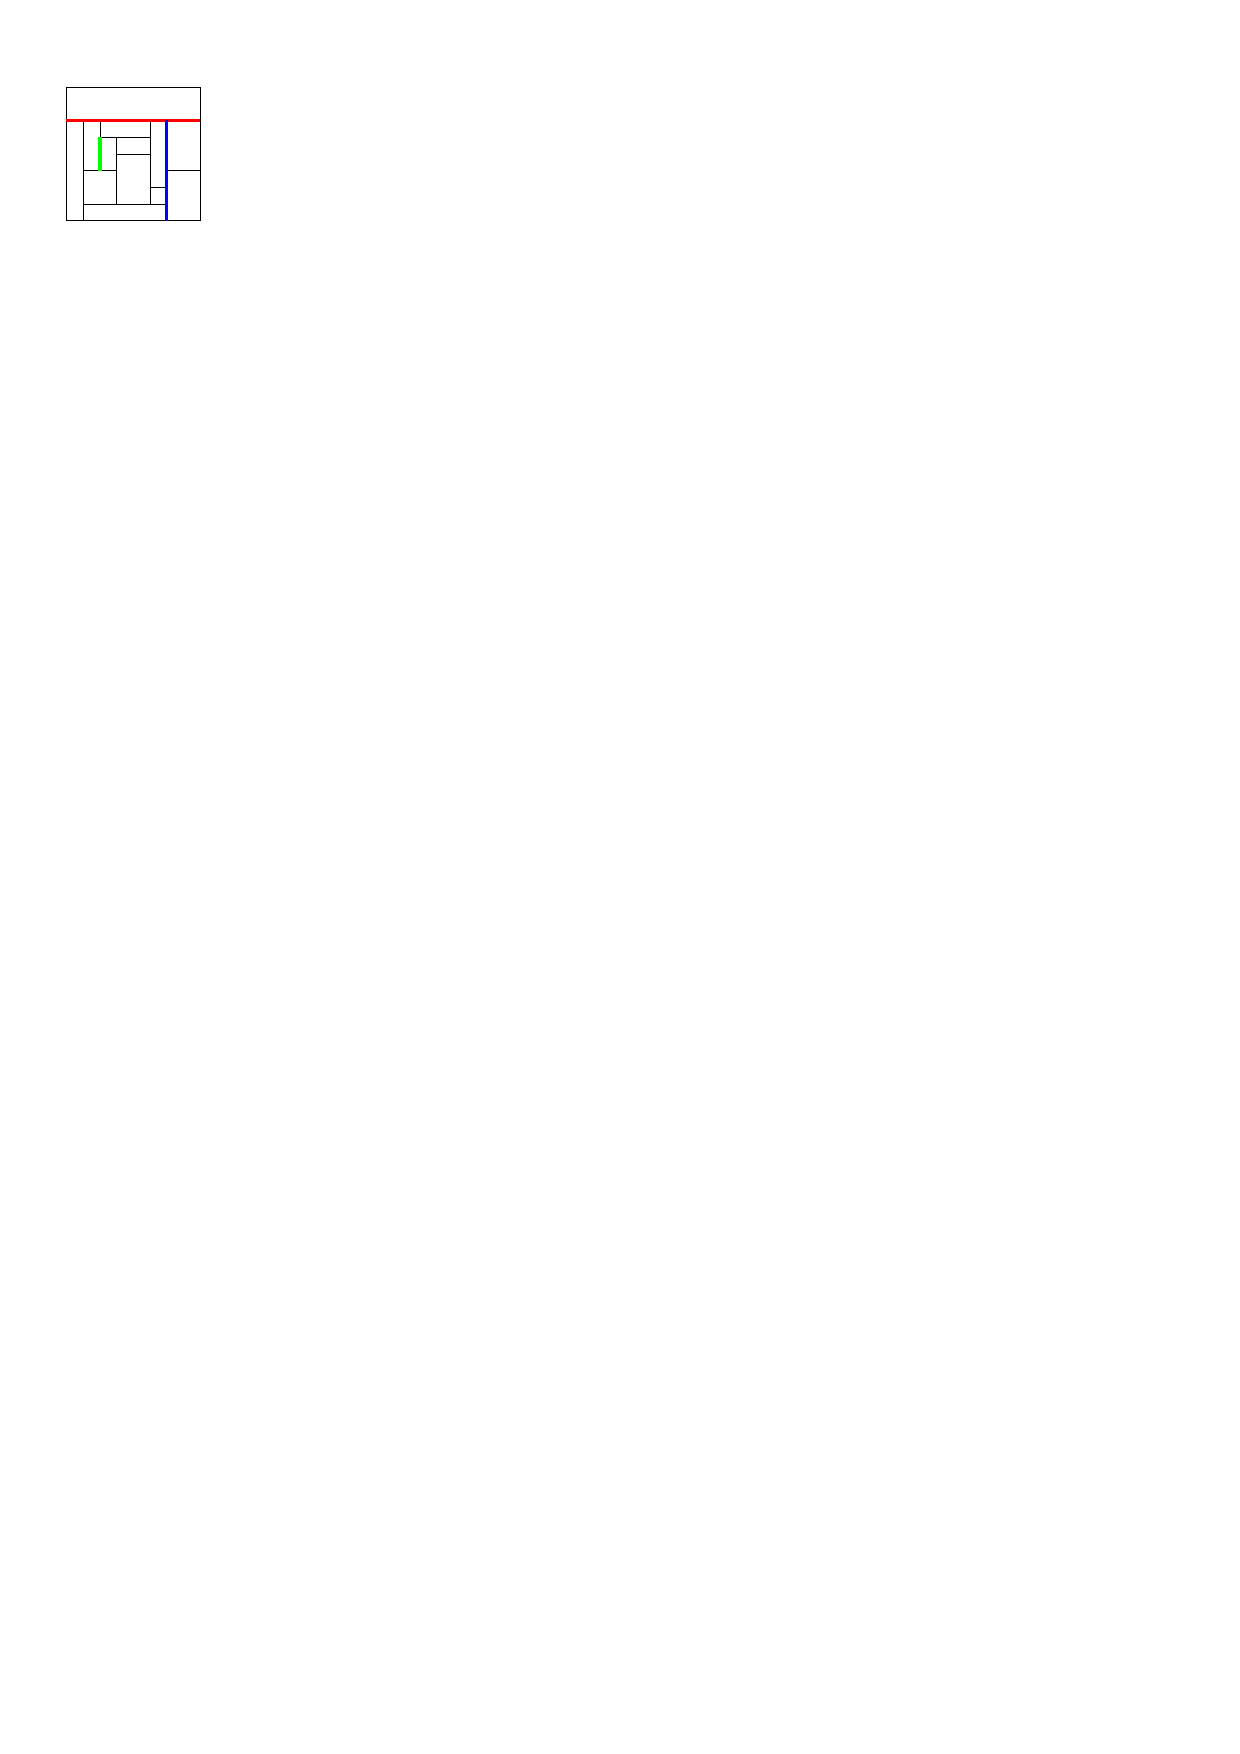
\includegraphics[scale=1]{rectangularDuals/img/segmentdefs}
\clearpage% page: 1

\includegraphics[scale=1]{rectangularDuals/img/vertonesided}
\clearpage% page: 2
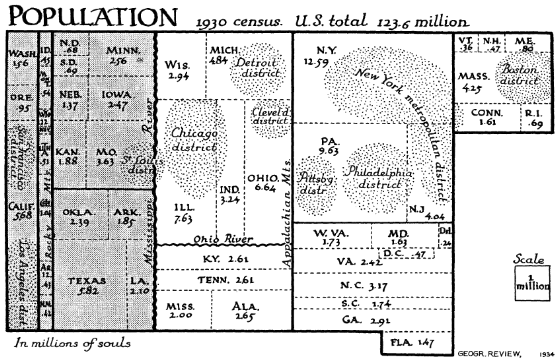
\includegraphics[scale=.5]{./introduction/img/cartogram.png}
\clearpage% page: 3
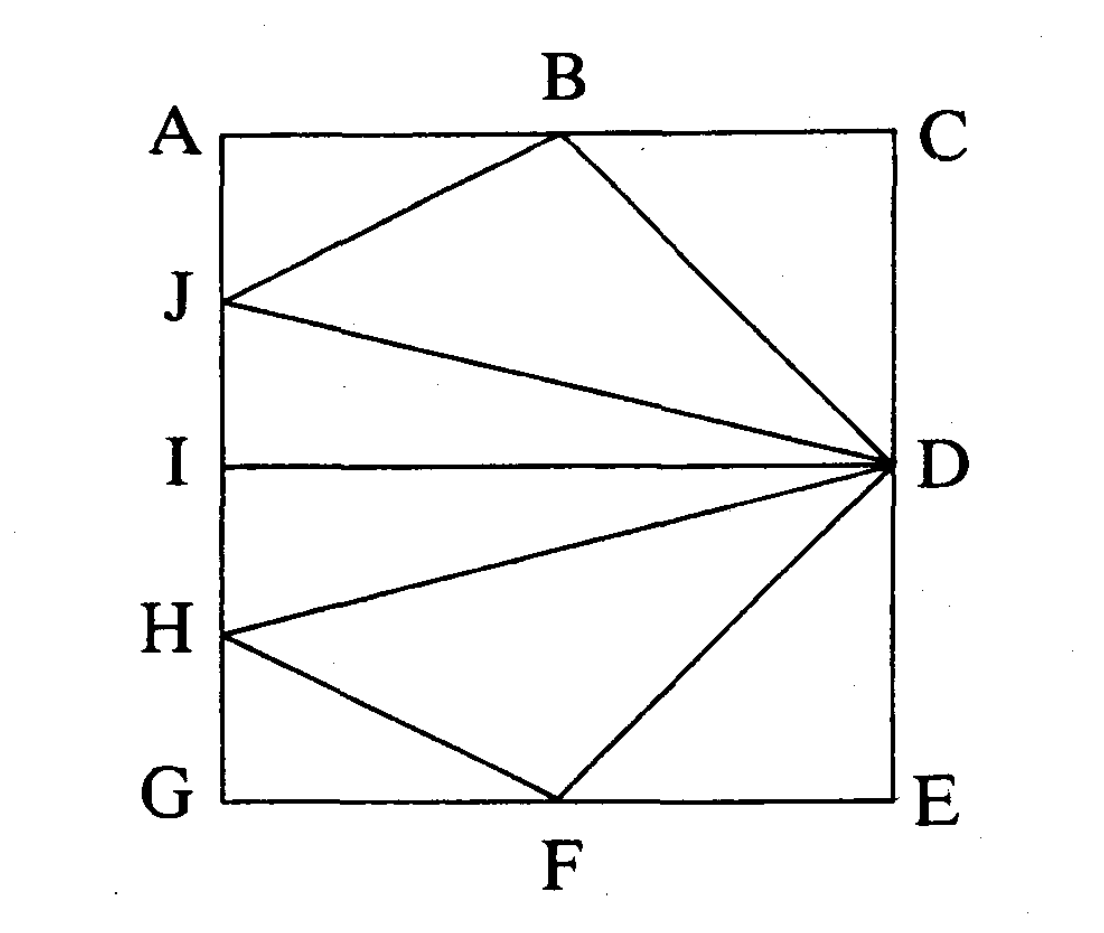
\includegraphics[scale=.15]{./introduction/img/rinsma.png}
\clearpage% page: 4
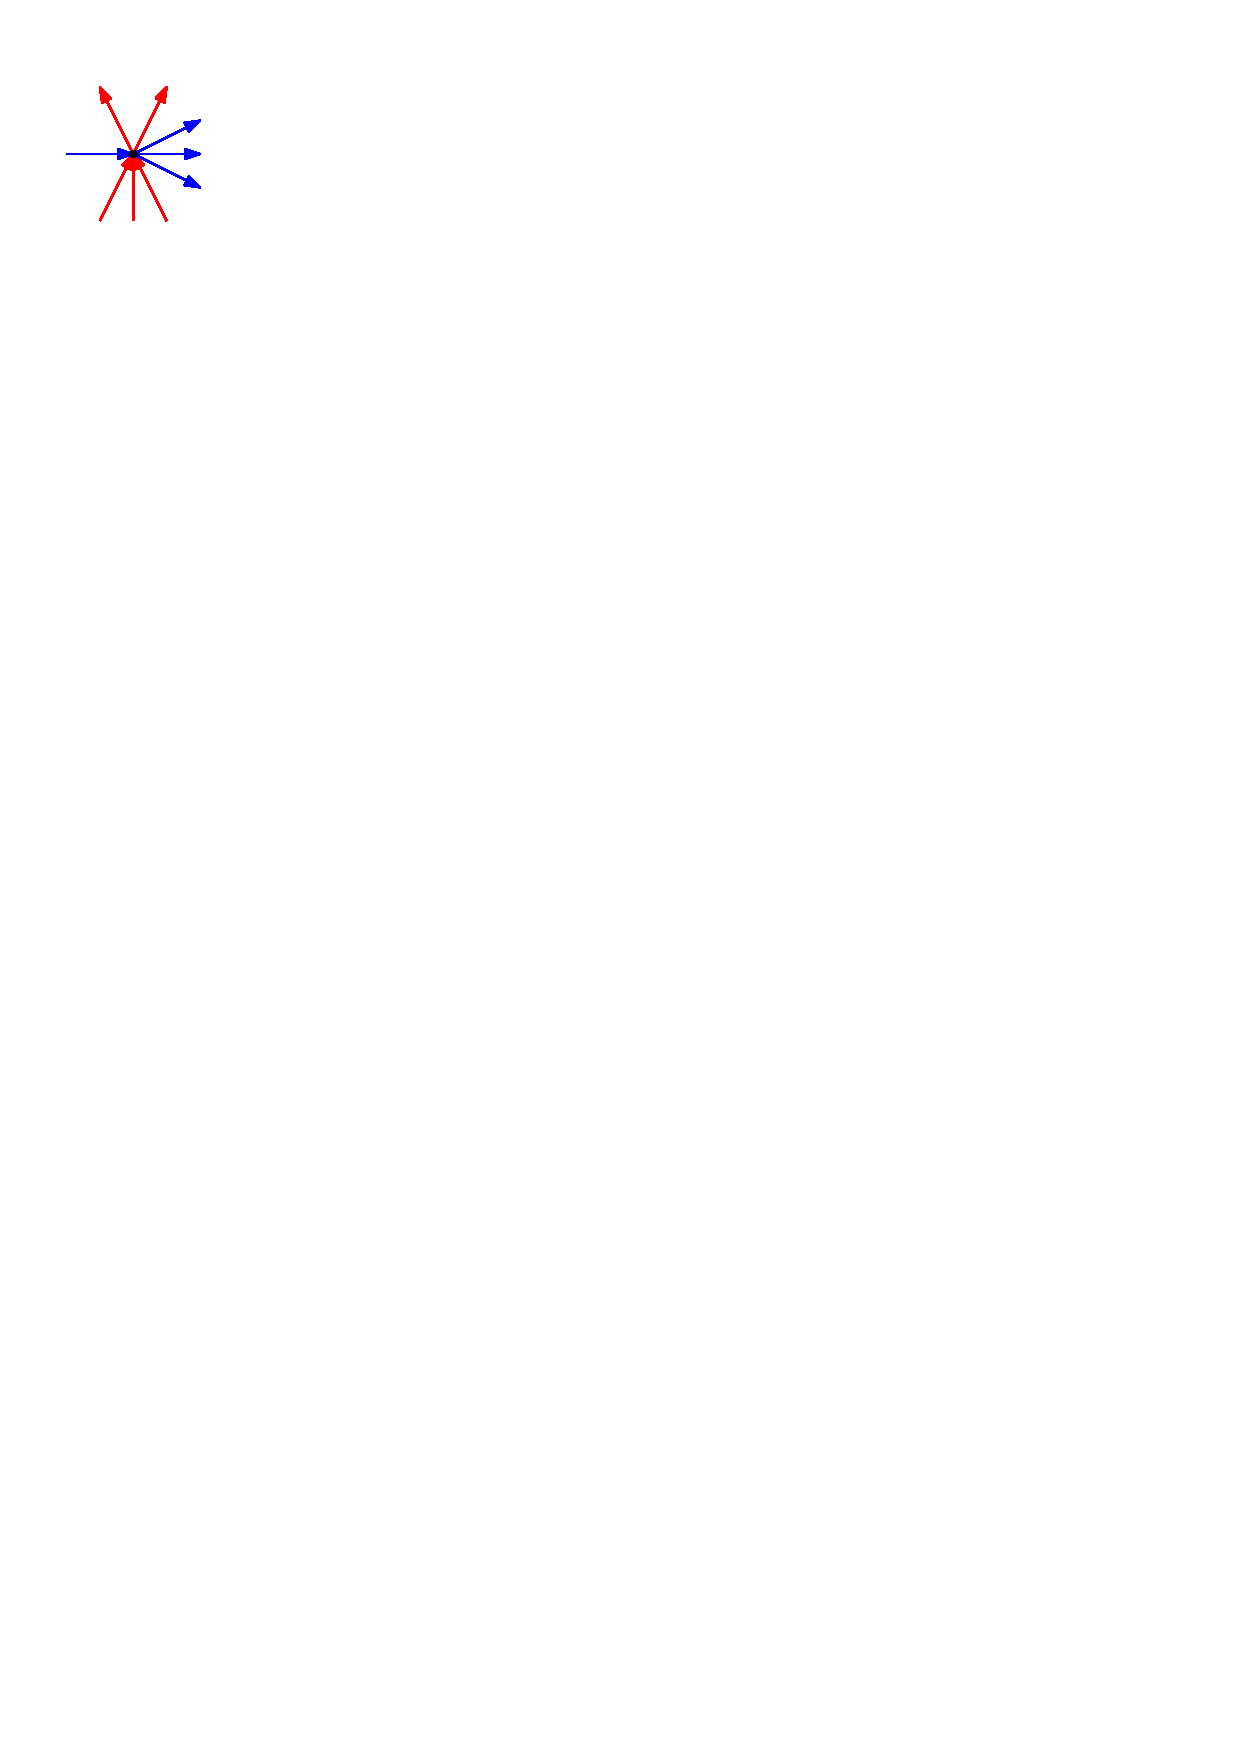
\includegraphics[width = \textwidth]{./rectangularDuals/img/interiorcondition.pdf}
\clearpage% page: 5
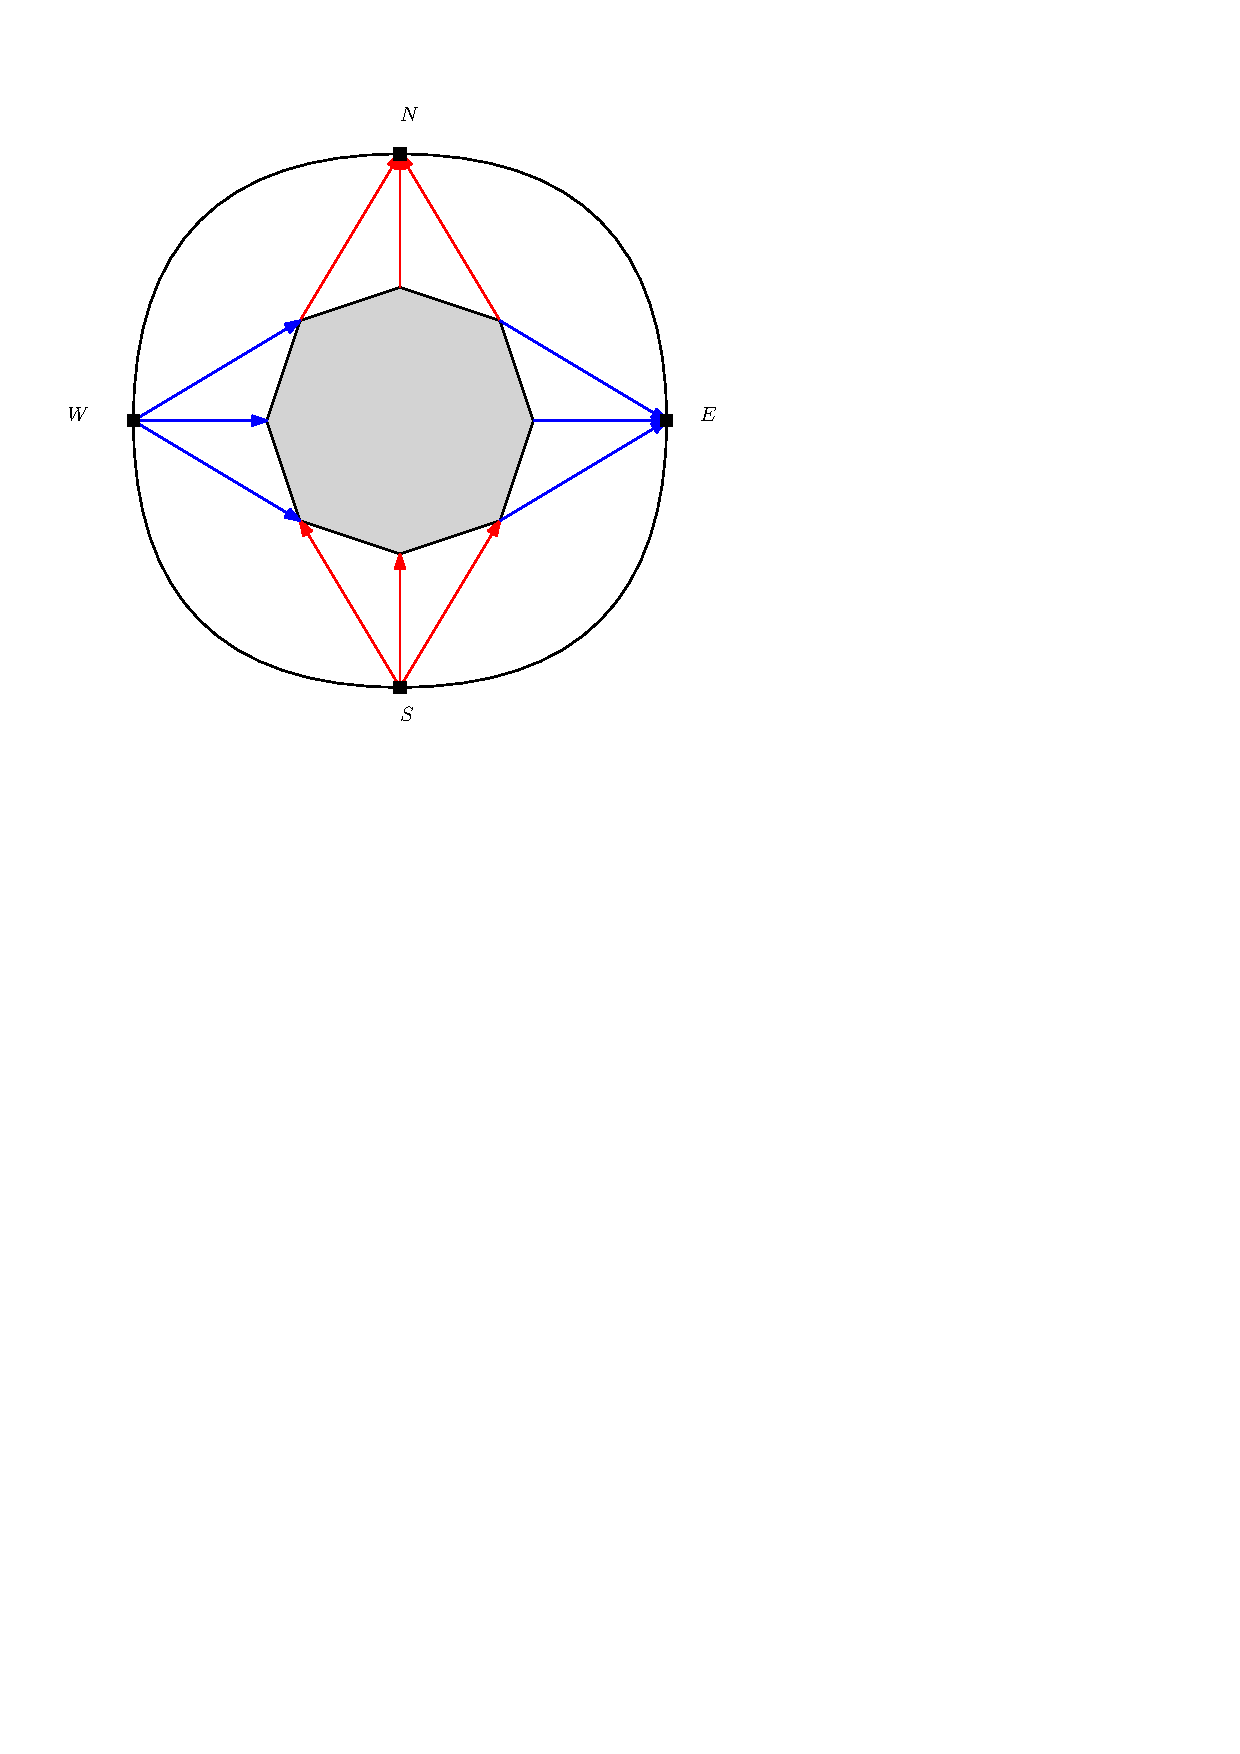
\includegraphics[width =\textwidth]{./rectangularDuals/img/exteriorCondition.pdf}
\clearpage% page: 6
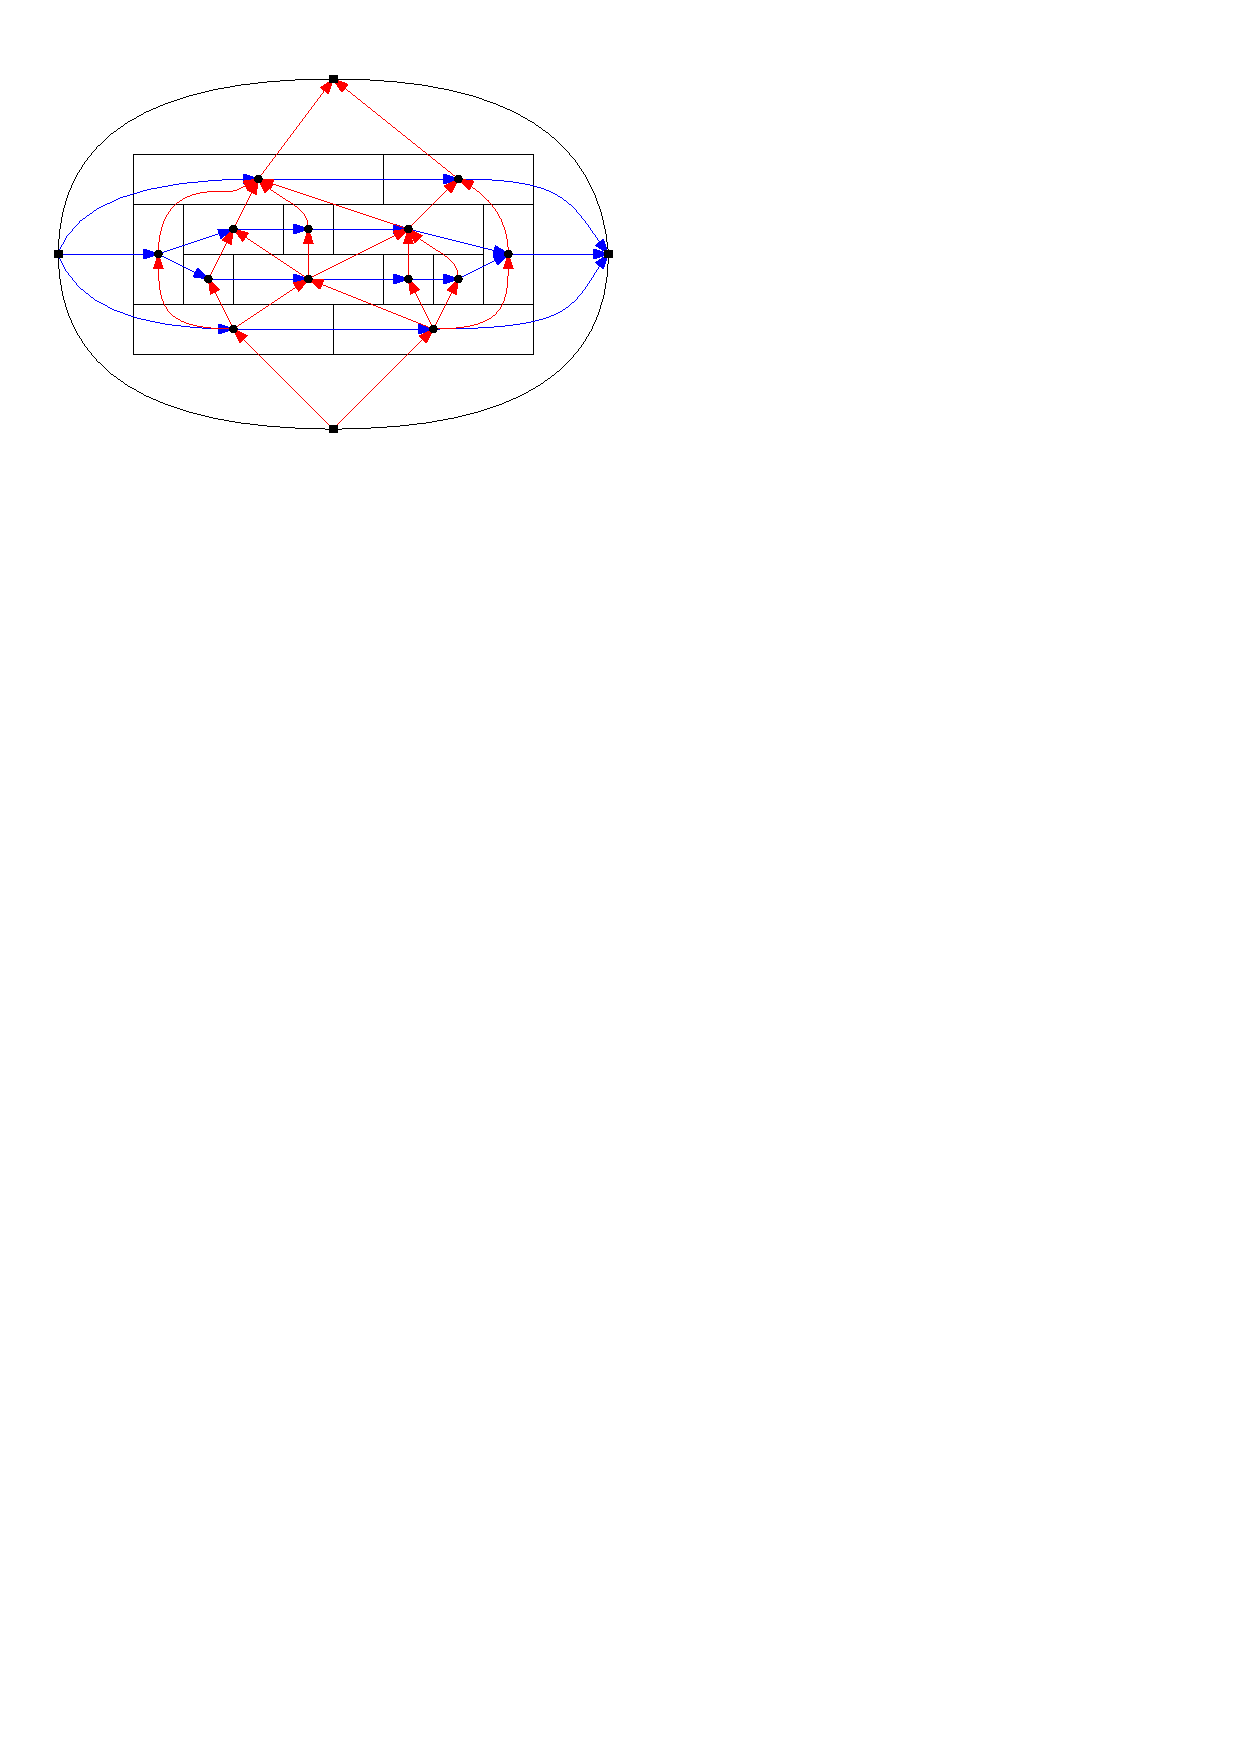
\includegraphics[scale=1]{rectangularDuals/img/relSegmentFaceRescale}
\clearpage% page: 7
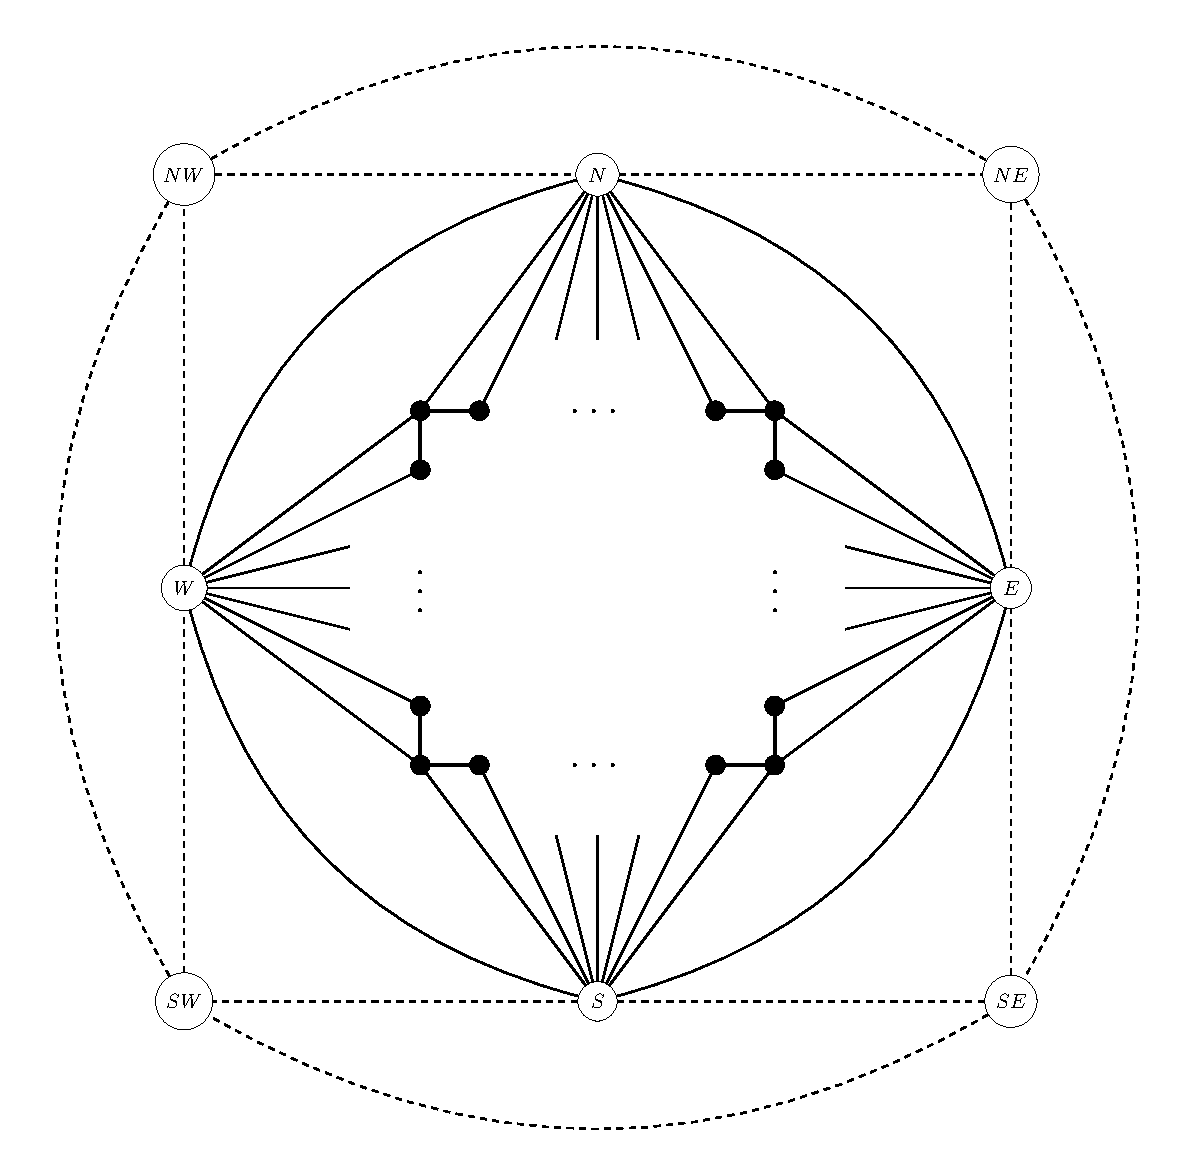
\includegraphics[scale=0.5]{fixExtension/img/scafold}
\clearpage% page: 8
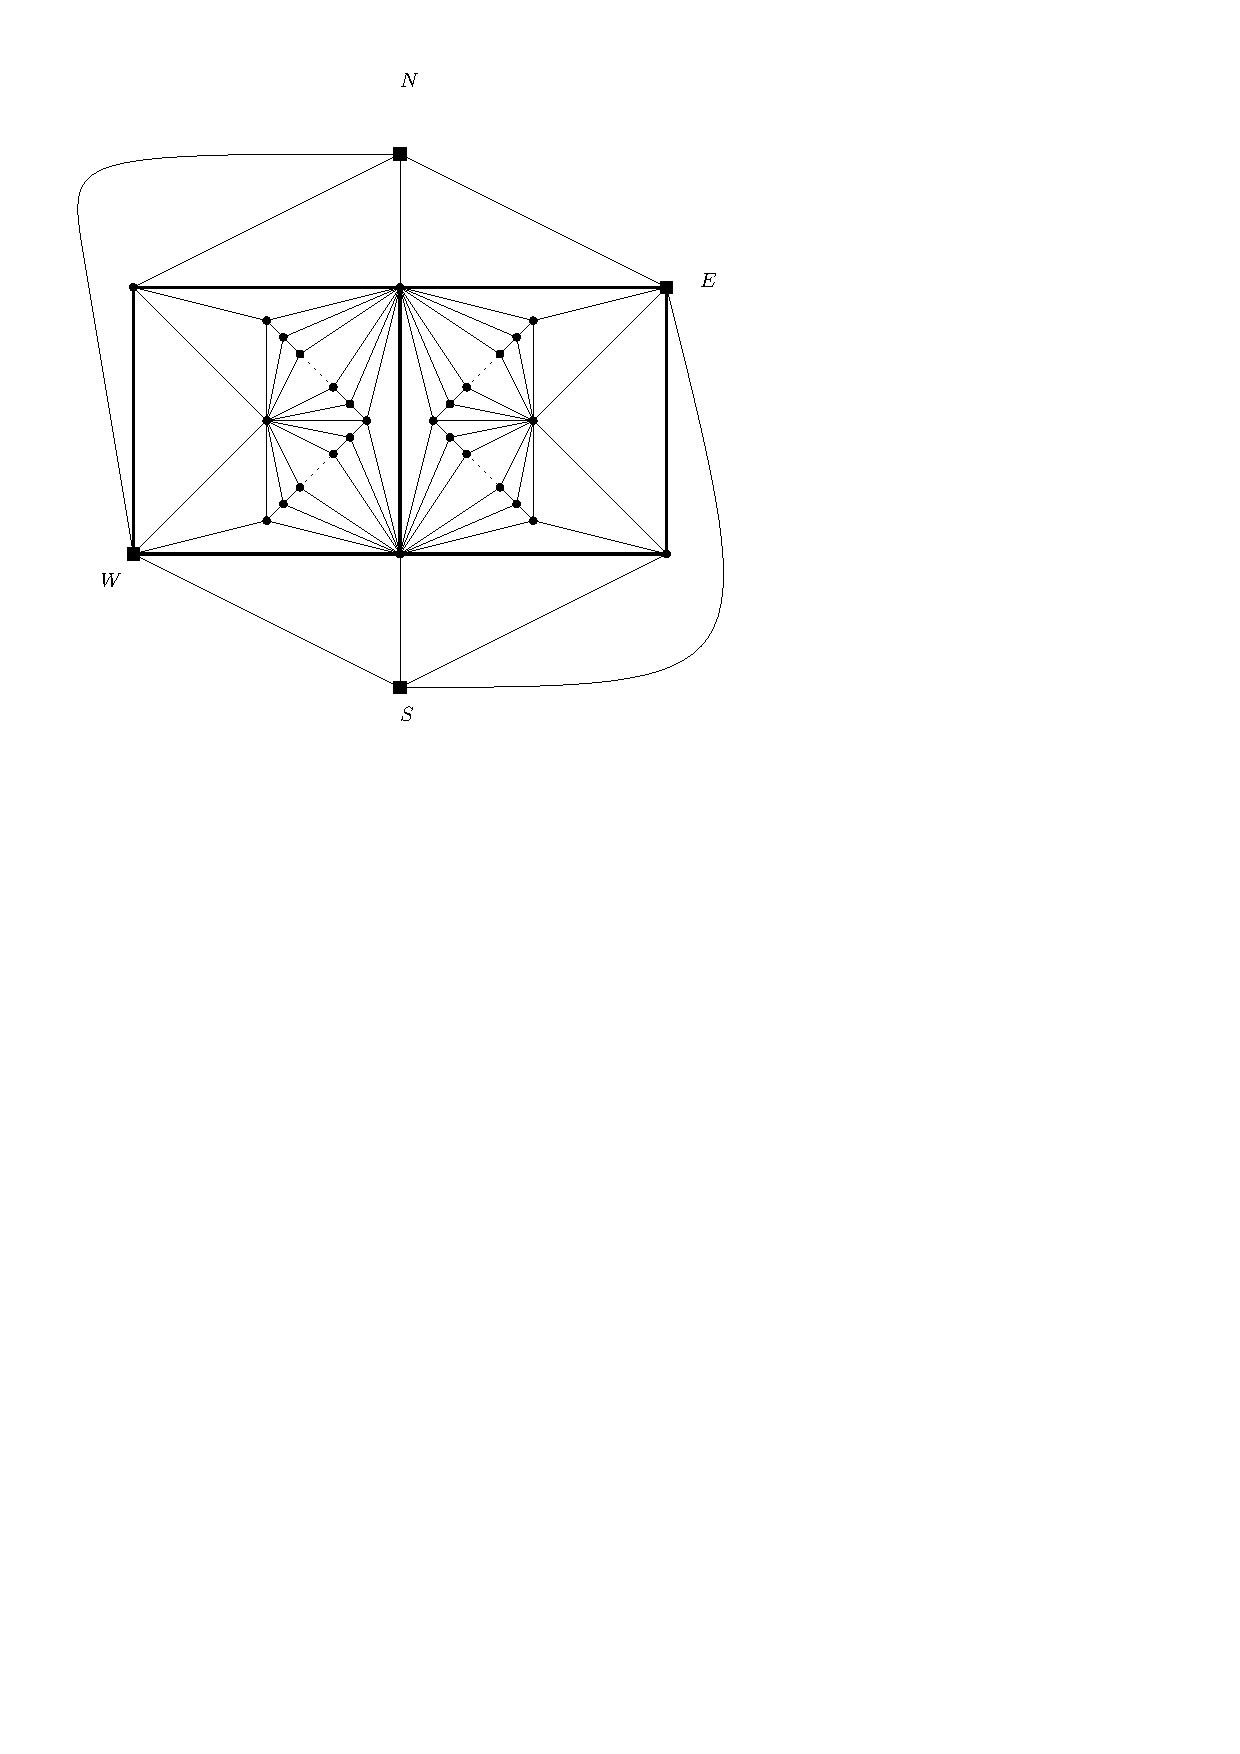
\includegraphics[scale=1]{fixExtension/img/manymanybase}
\clearpage% page: 9
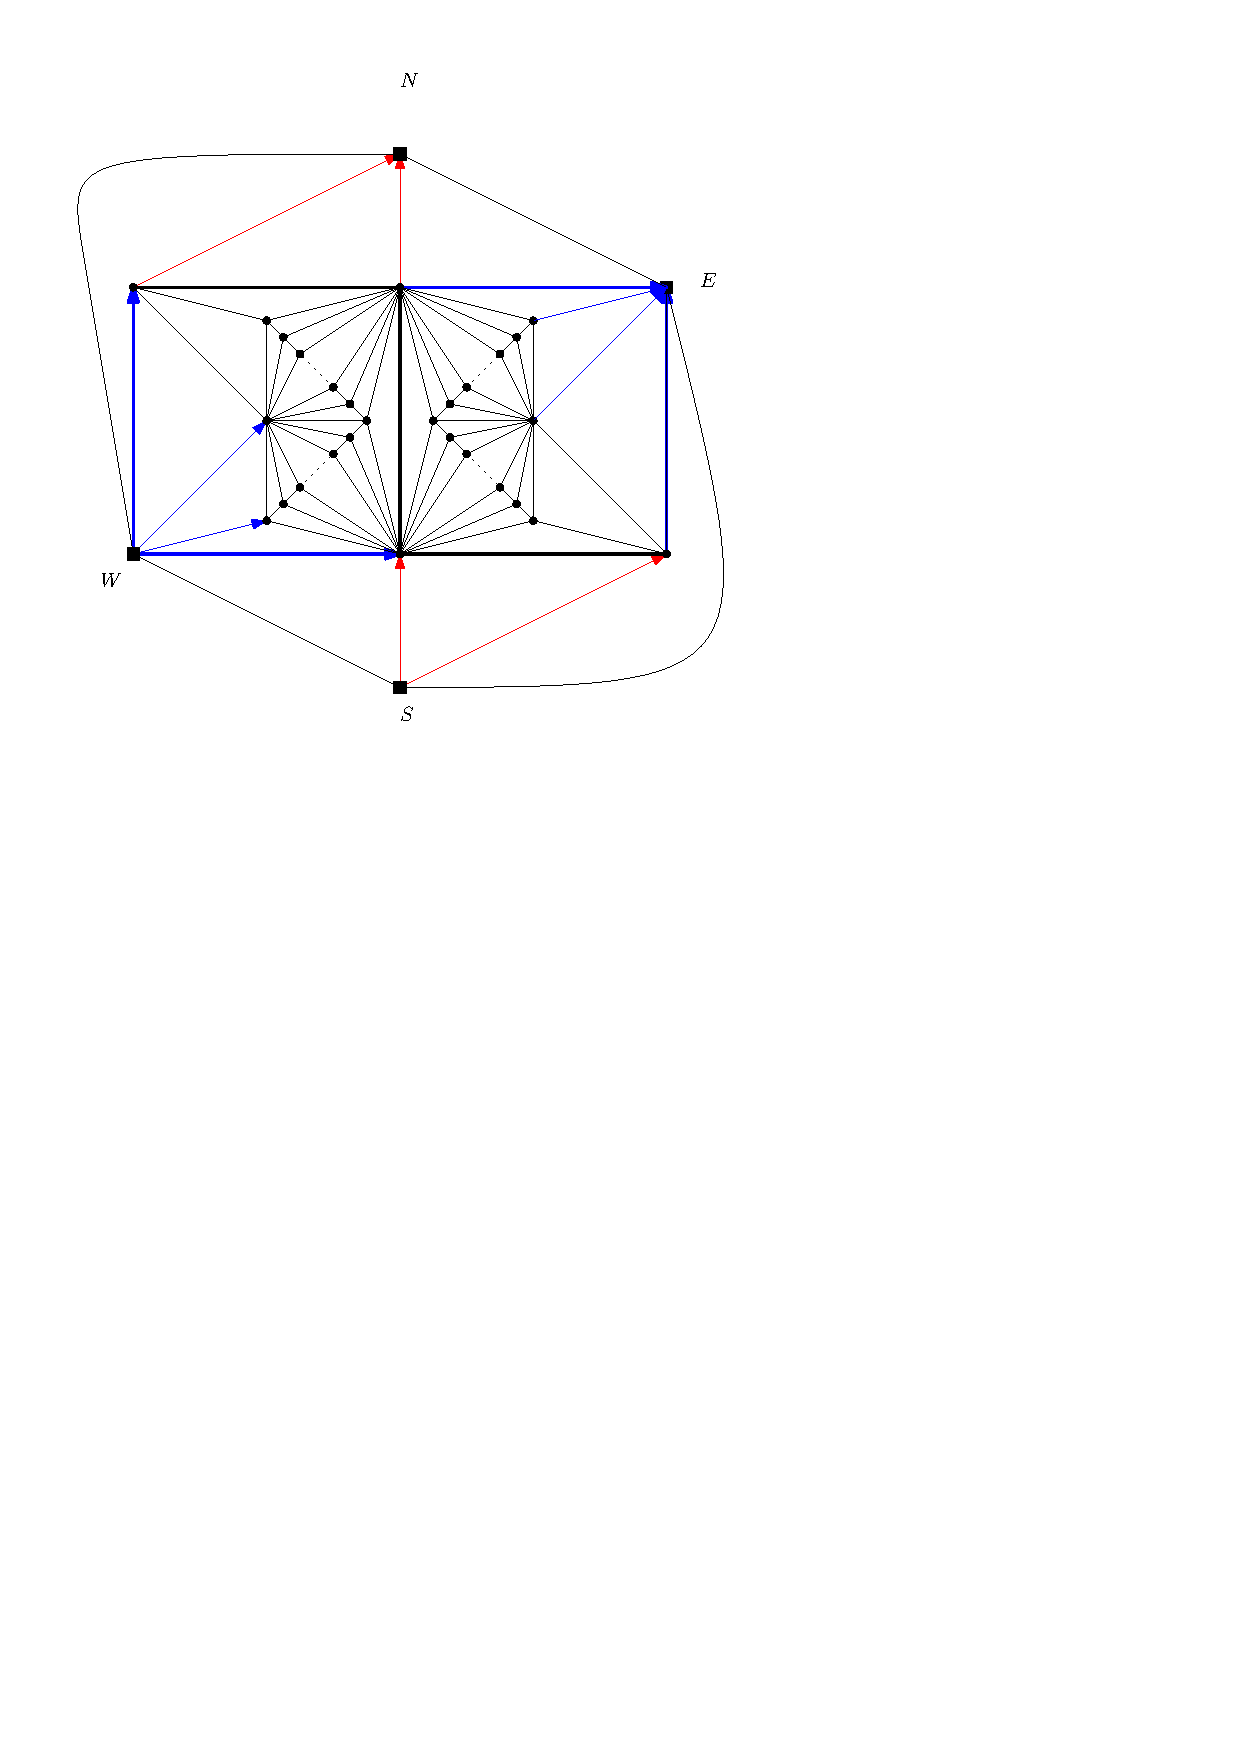
\includegraphics[width=\textwidth]{fixExtension/img/manymany1}
\clearpage% page: 10
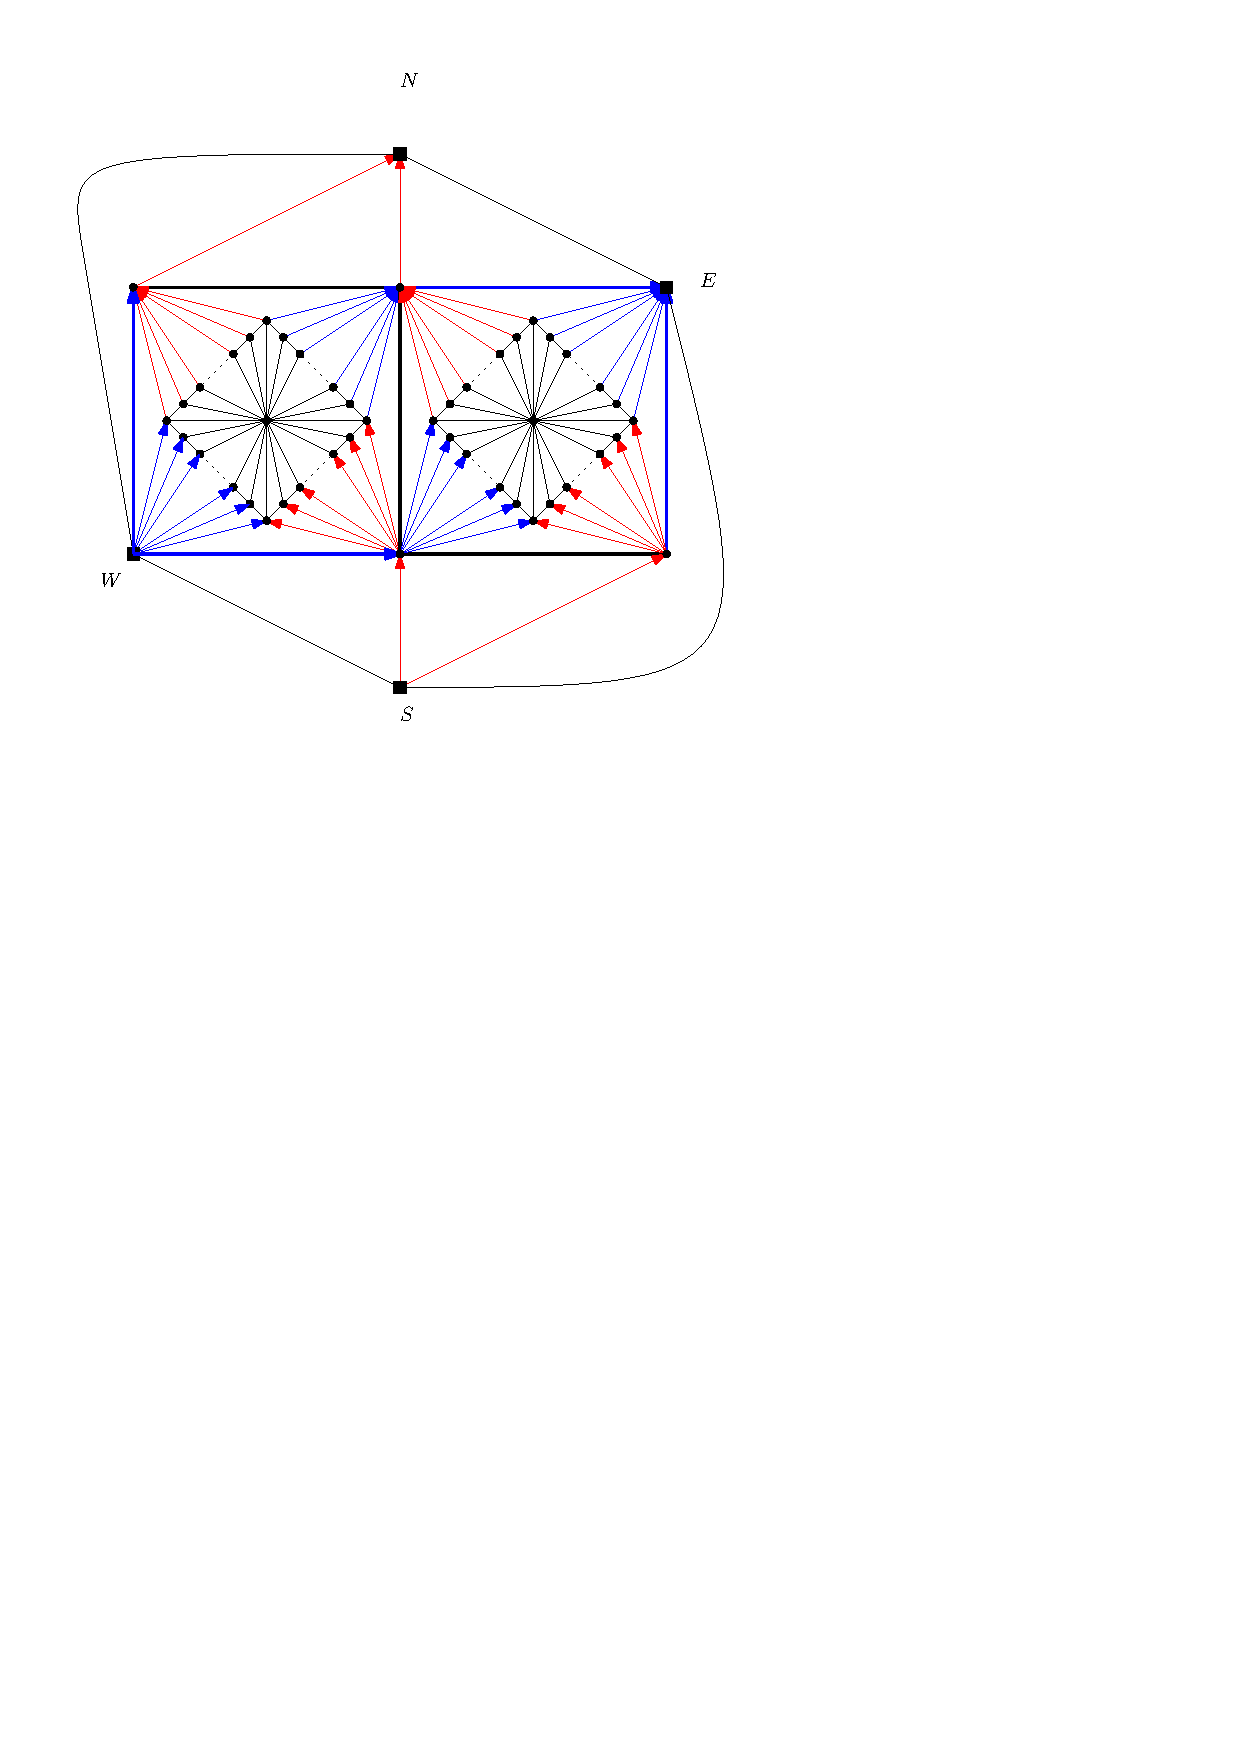
\includegraphics[width=\textwidth]{fixExtension/img/manymany2}
\clearpage% page: 11
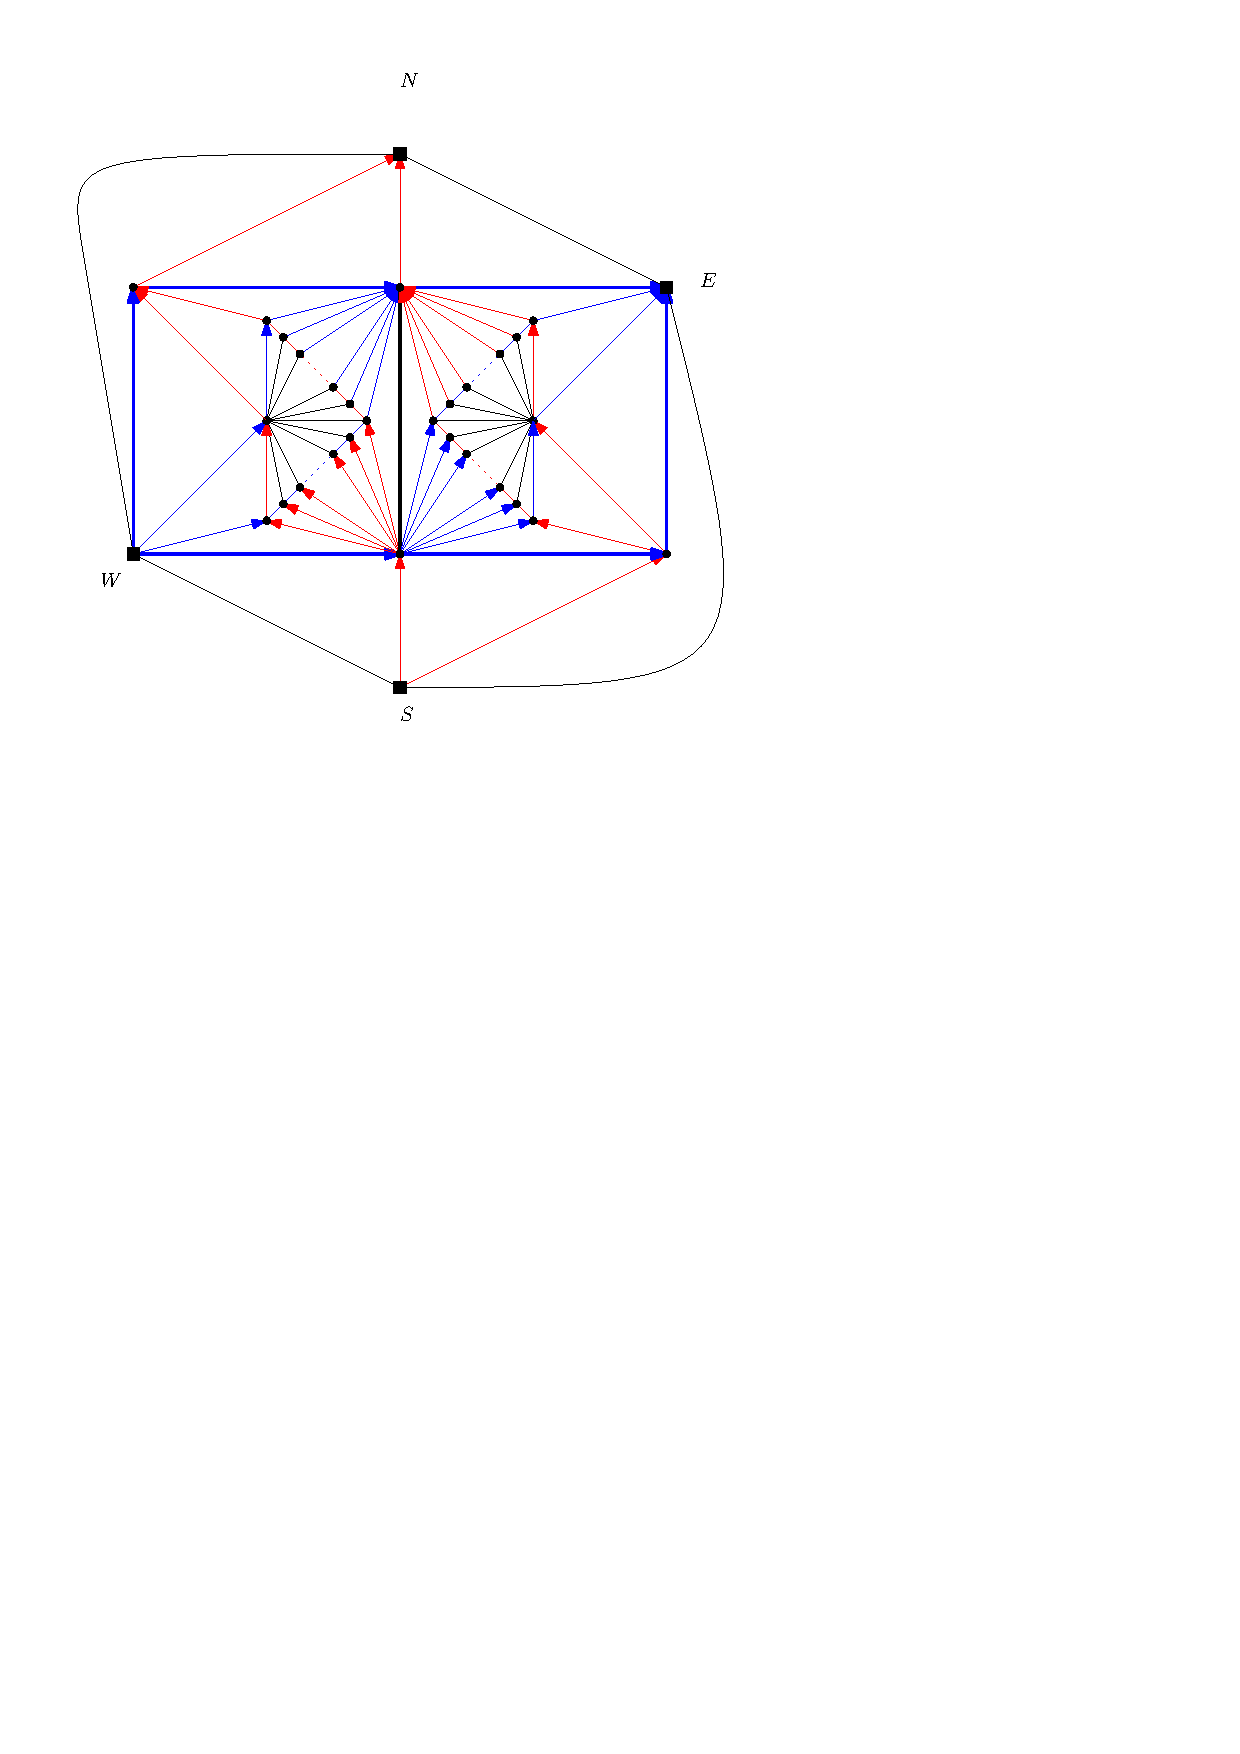
\includegraphics[width=\textwidth]{fixExtension/img/manymany3}
\clearpage% page: 12
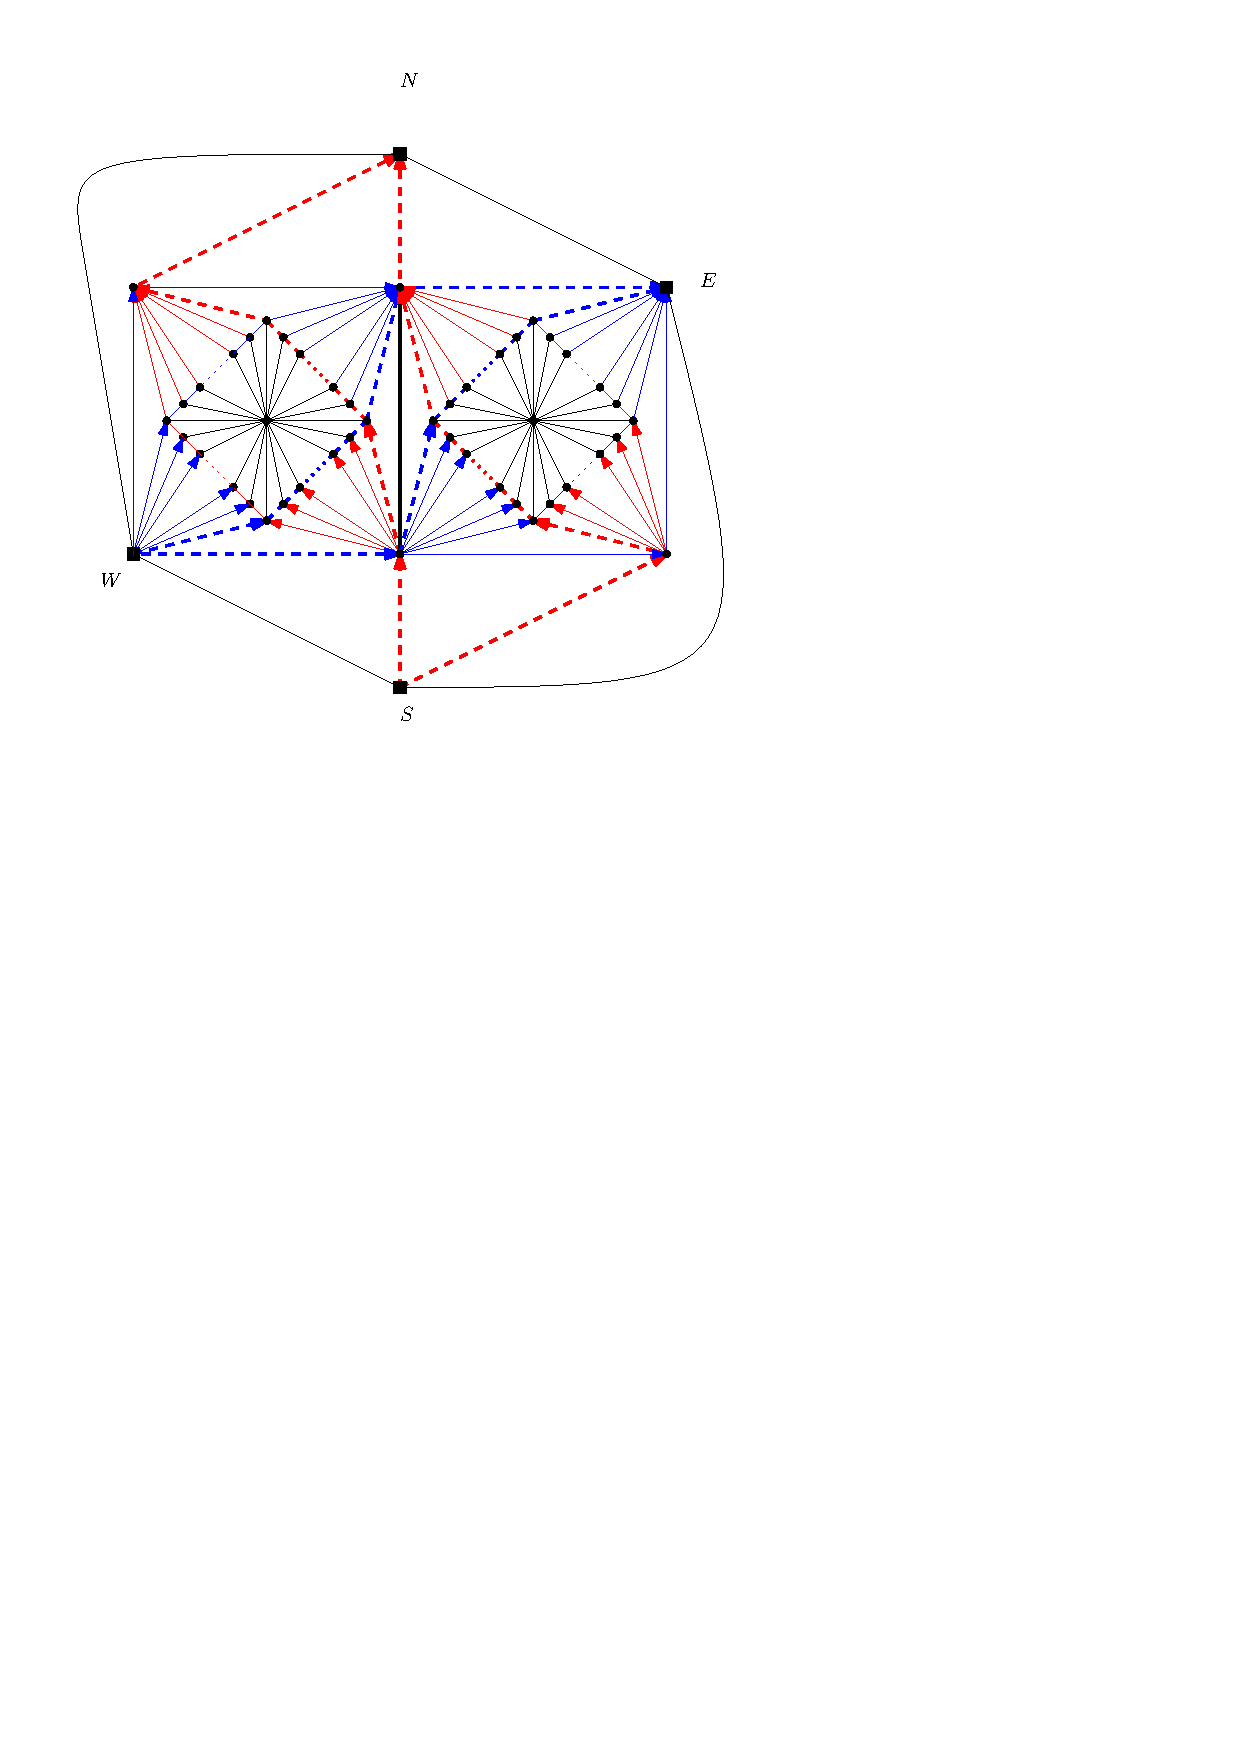
\includegraphics[scale=1]{fixExtension/img/manymany4}
\clearpage% page: 13
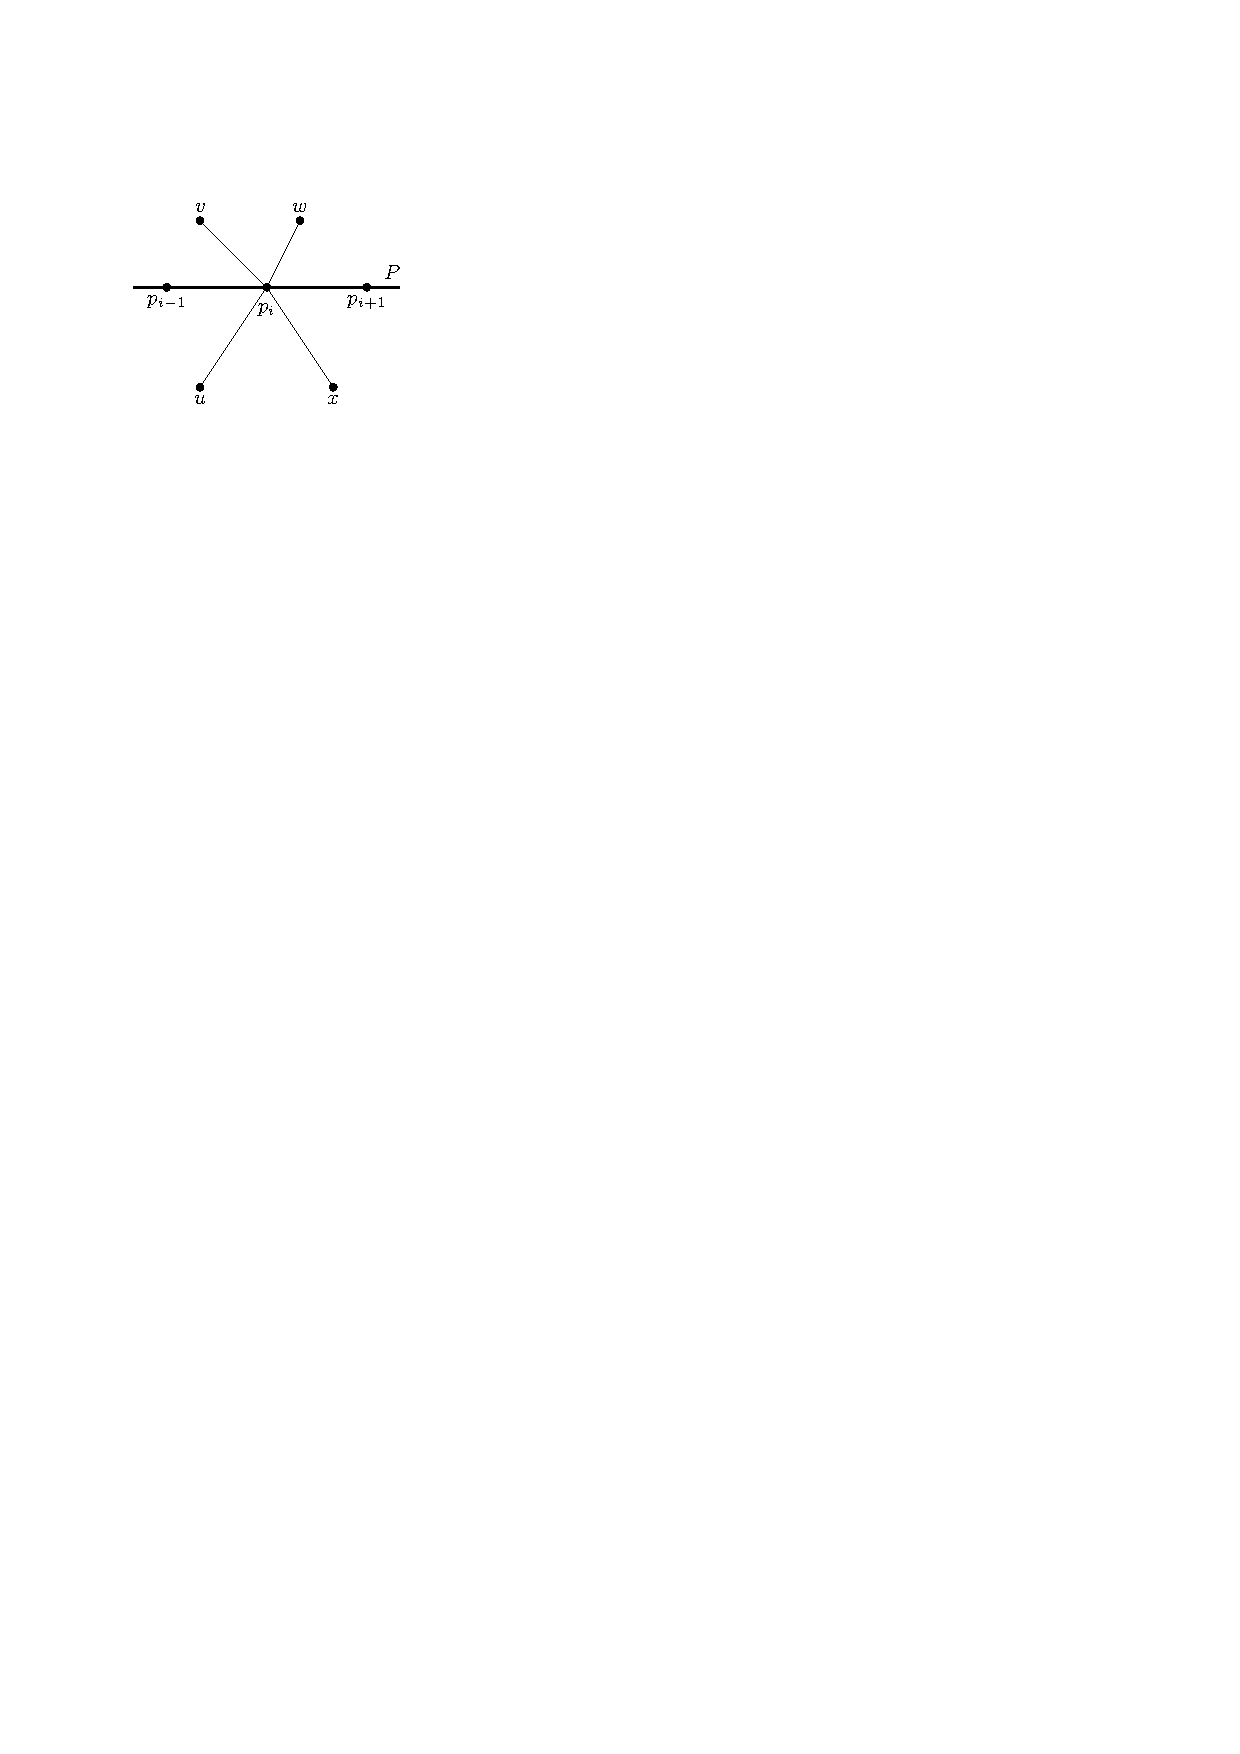
\includegraphics[scale=1]{unifiedAlgo/img/rightNeighbourwalk/rotation}
\clearpage% page: 14
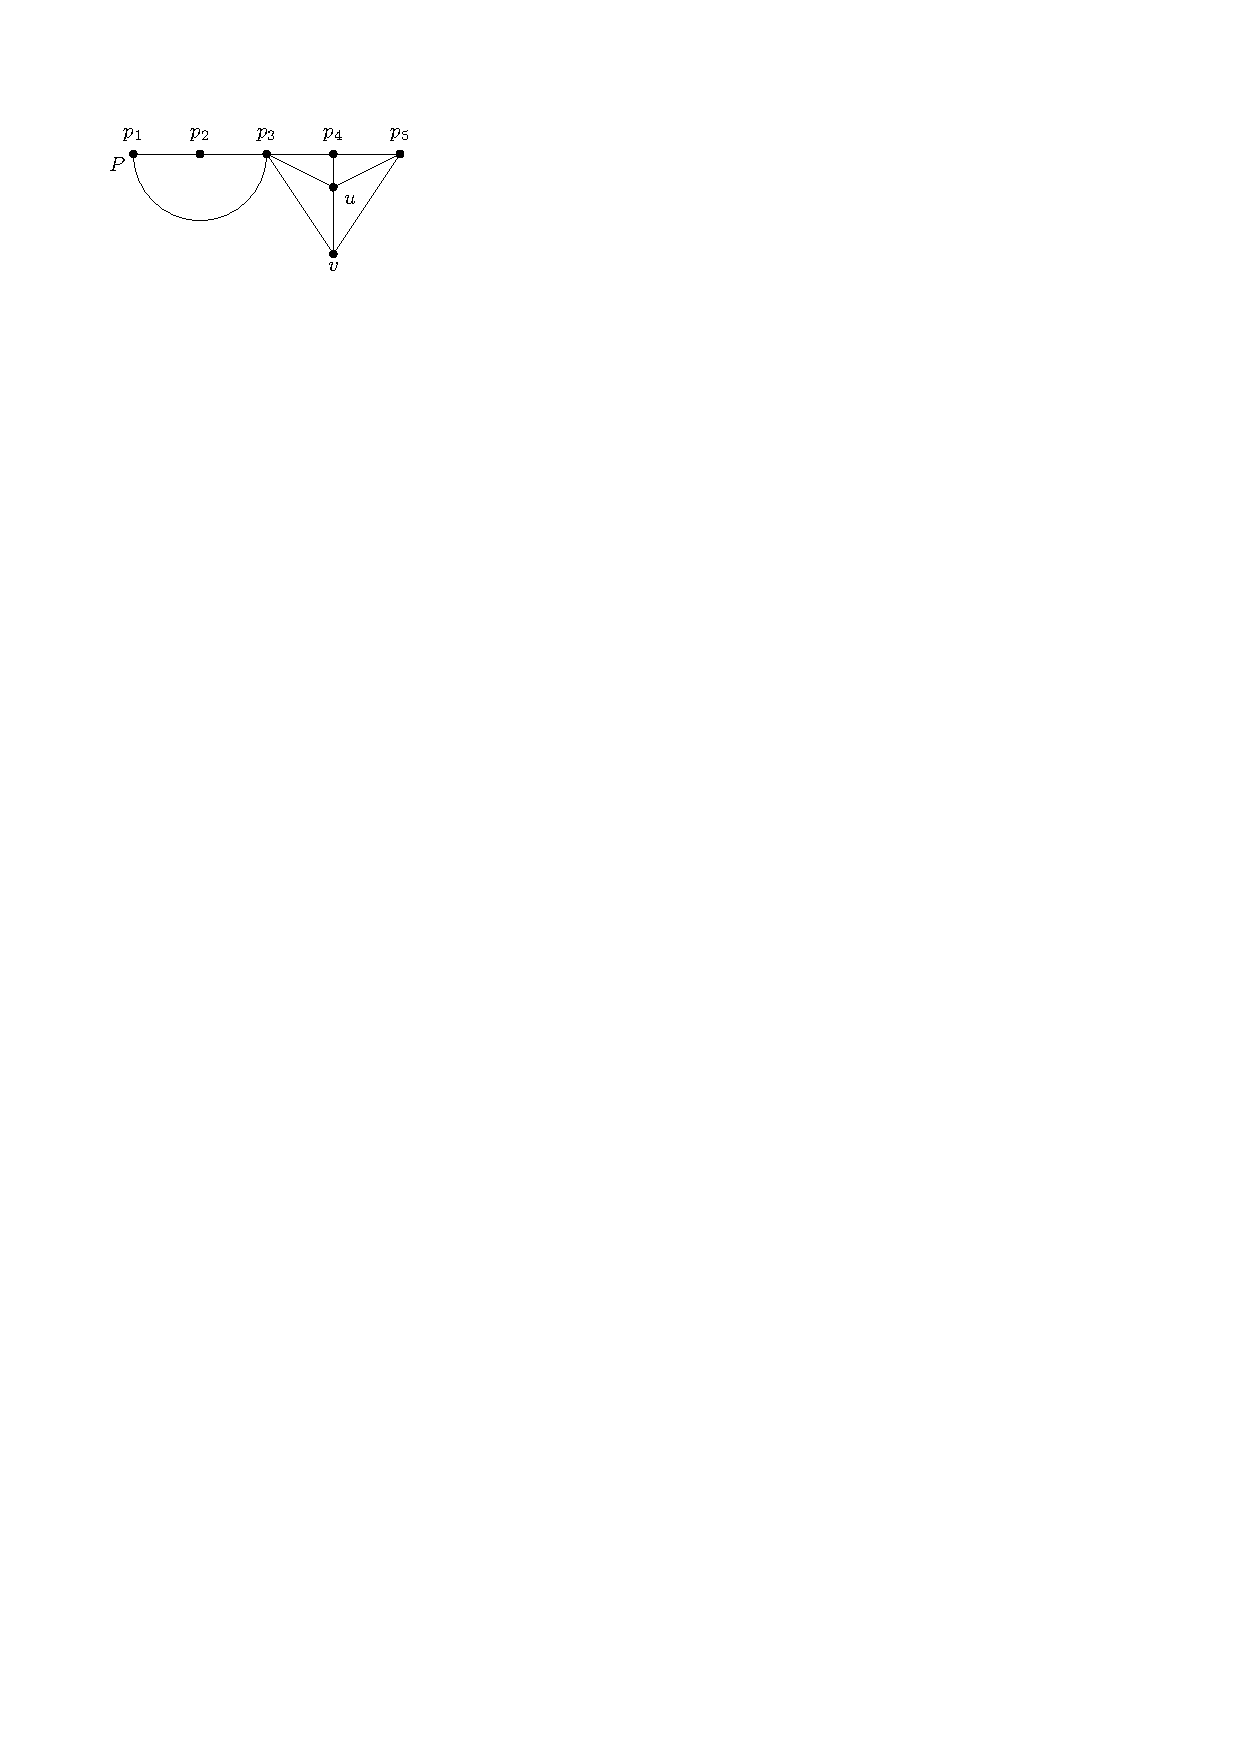
\includegraphics[scale=1]{./unifiedAlgo/img/rightNeighbourwalk/chords.pdf}
\clearpage% page: 15
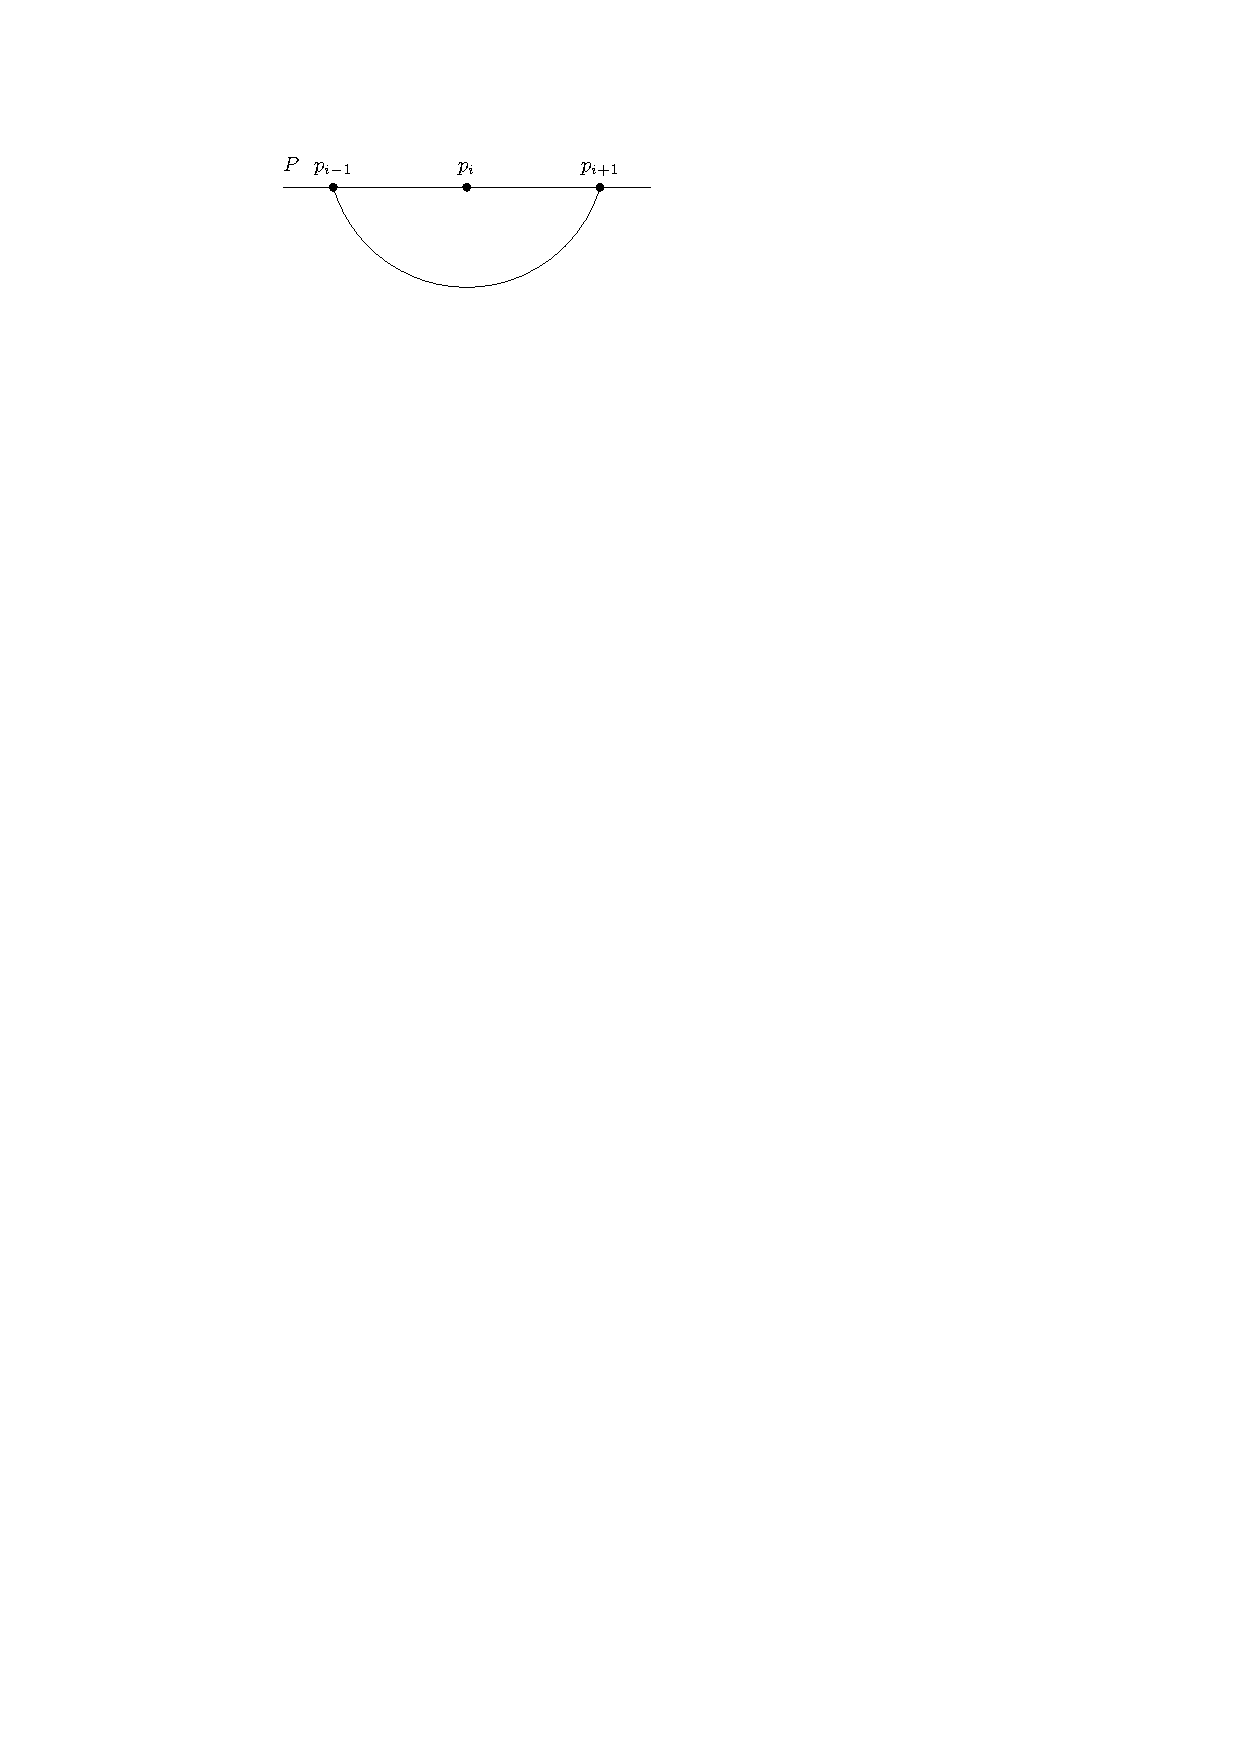
\includegraphics[scale=1]{./unifiedAlgo/img/rightNeighbourwalk/pHasRightNeighbor.pdf}
\clearpage% page: 16
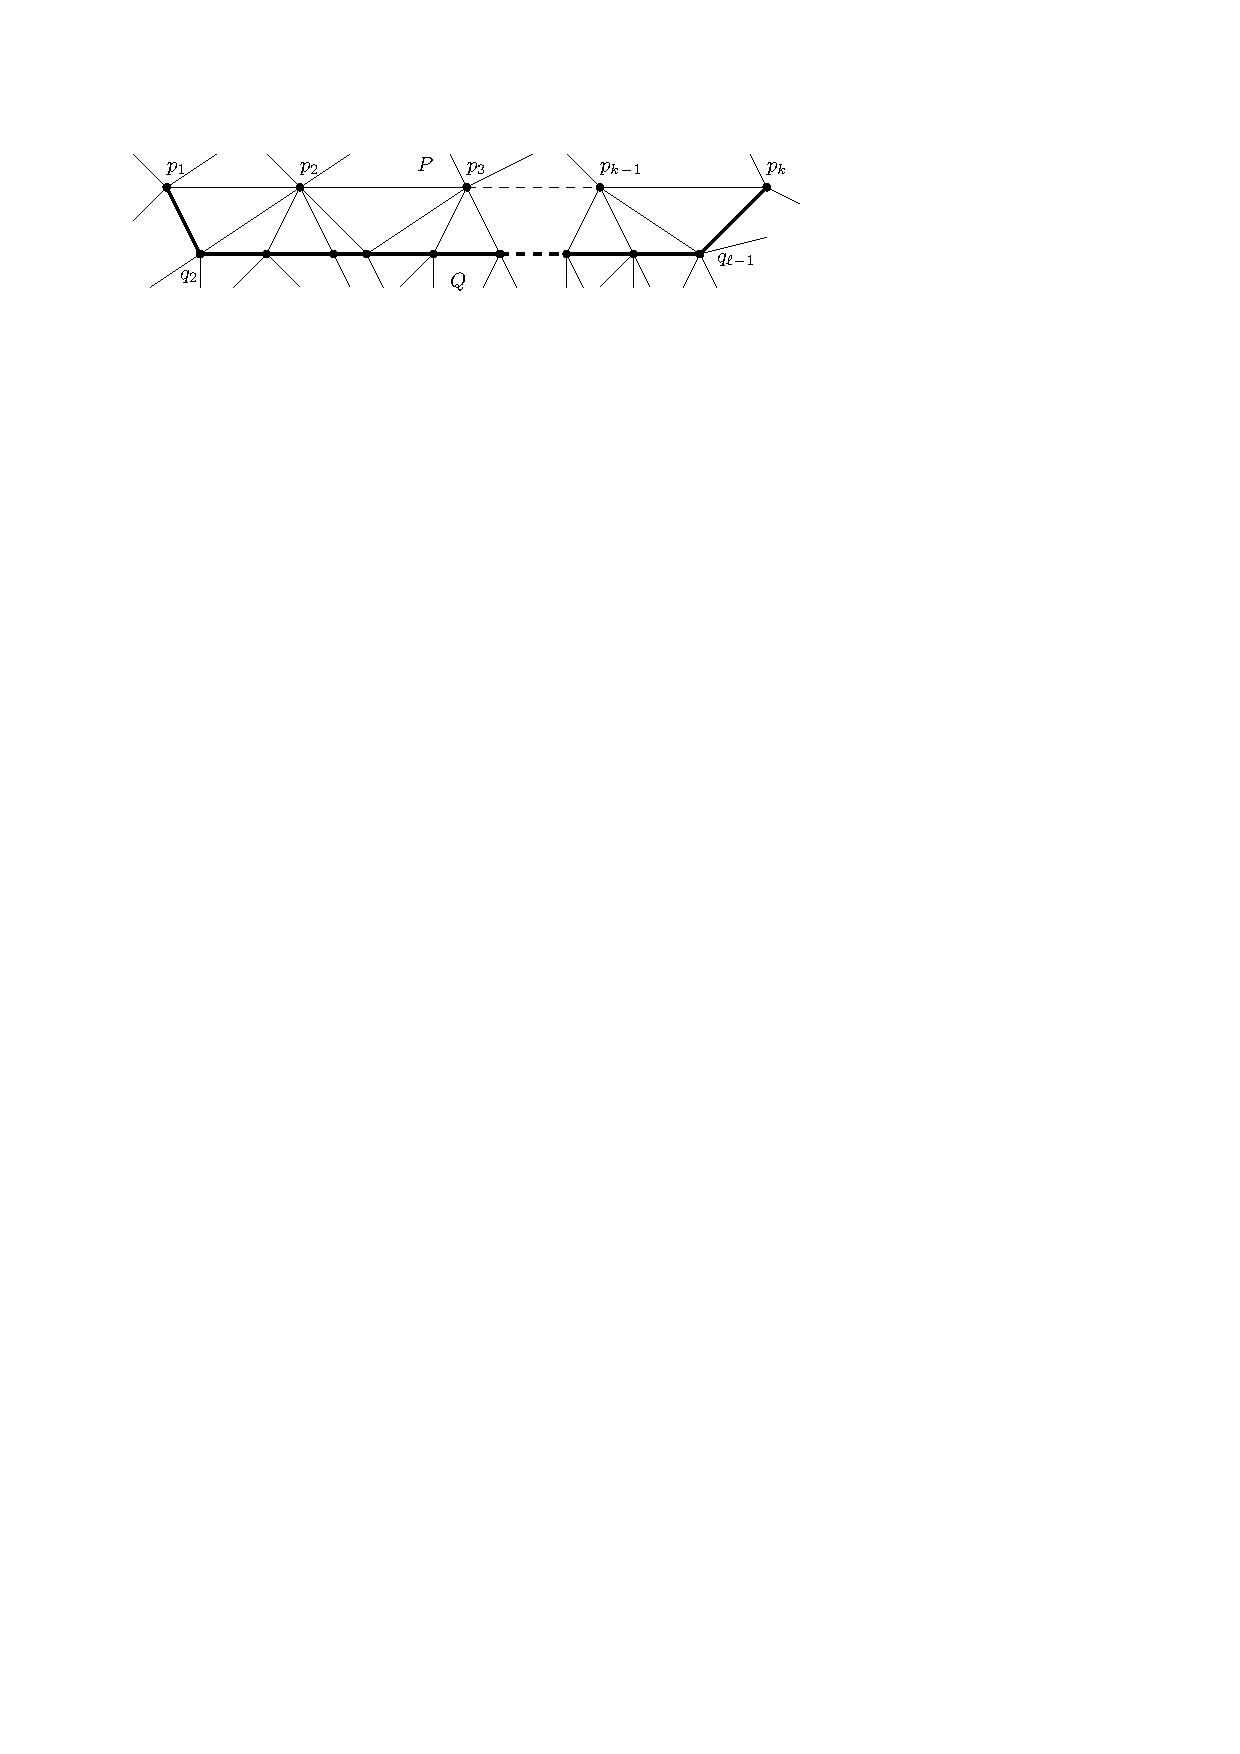
\includegraphics[scale=1]{./unifiedAlgo/img/rightNeighbourwalk/neighborPath.pdf}
\clearpage% page: 17
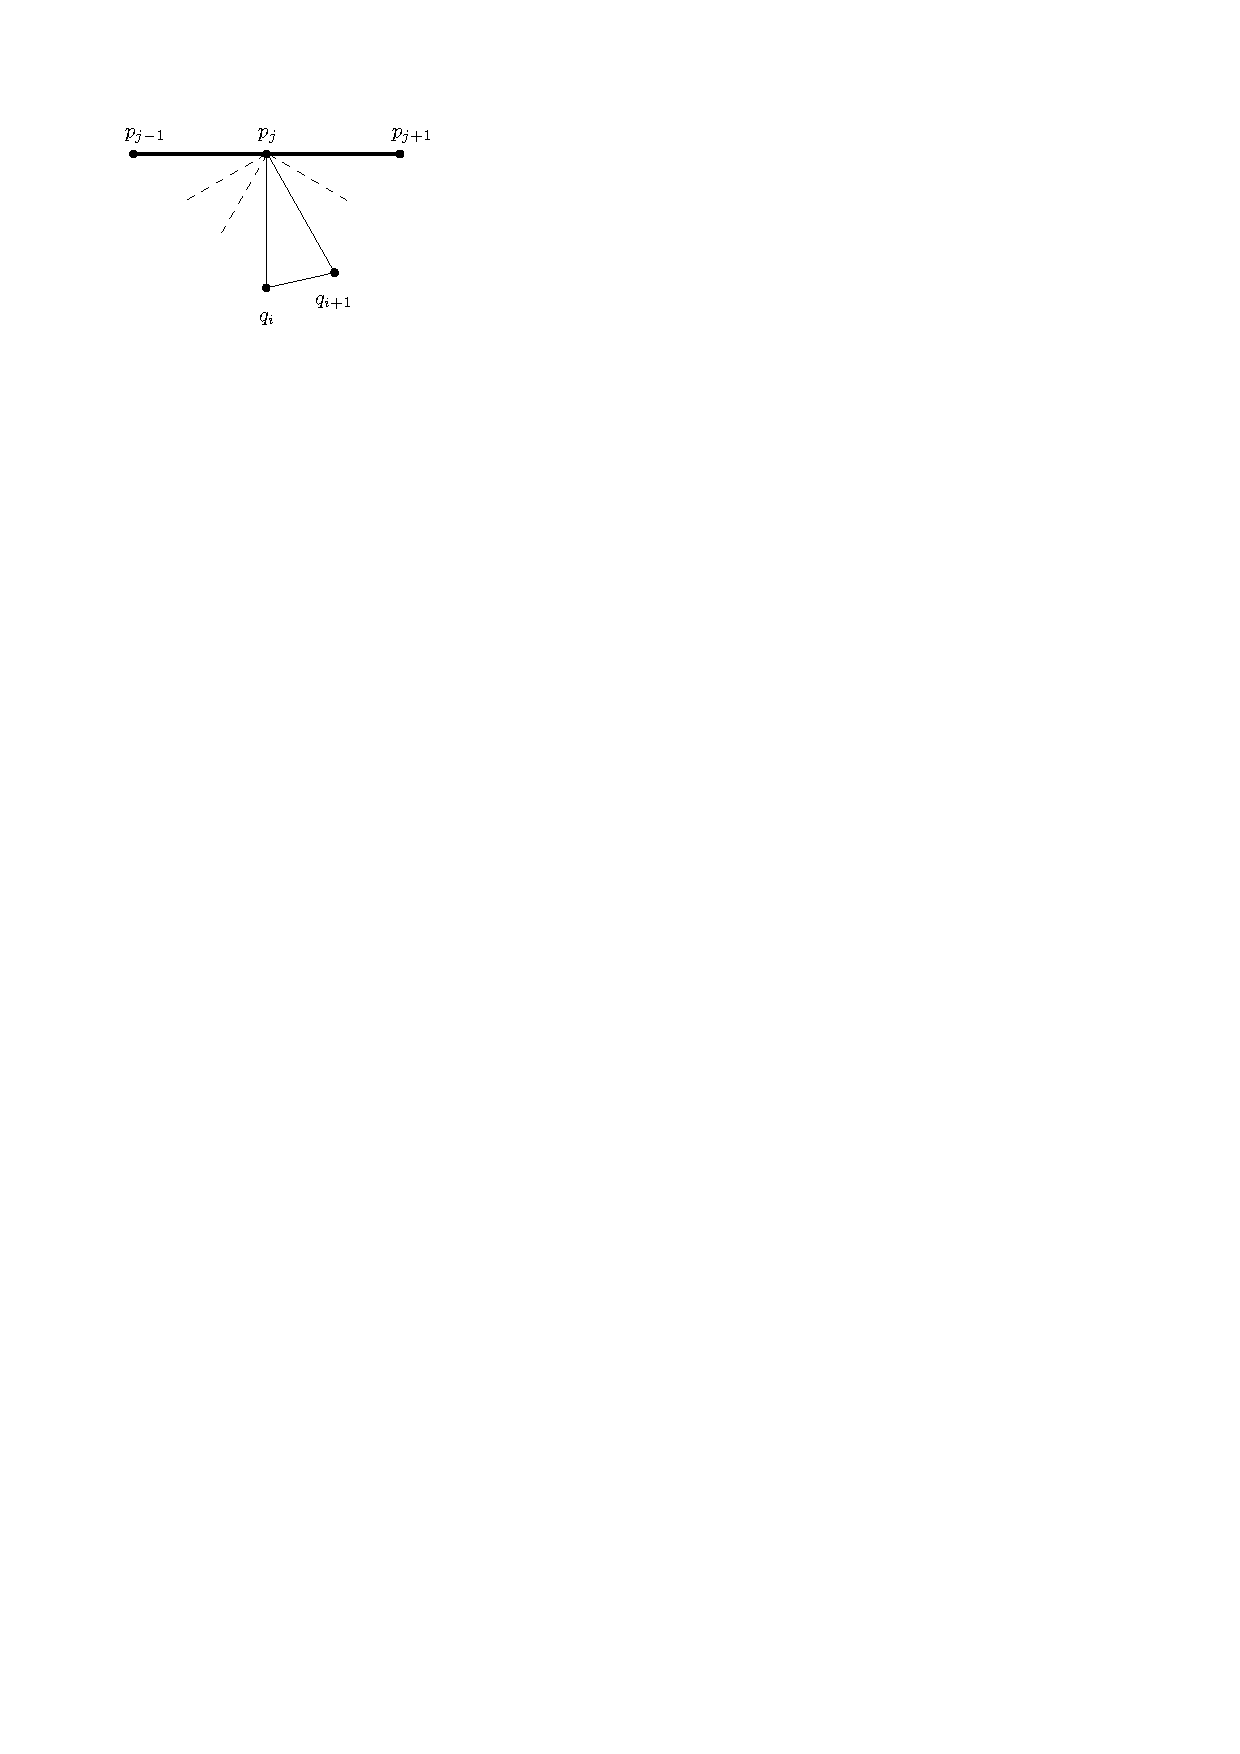
\includegraphics[width=\linewidth]{unifiedAlgo/img/walkProofA}
\clearpage% page: 18
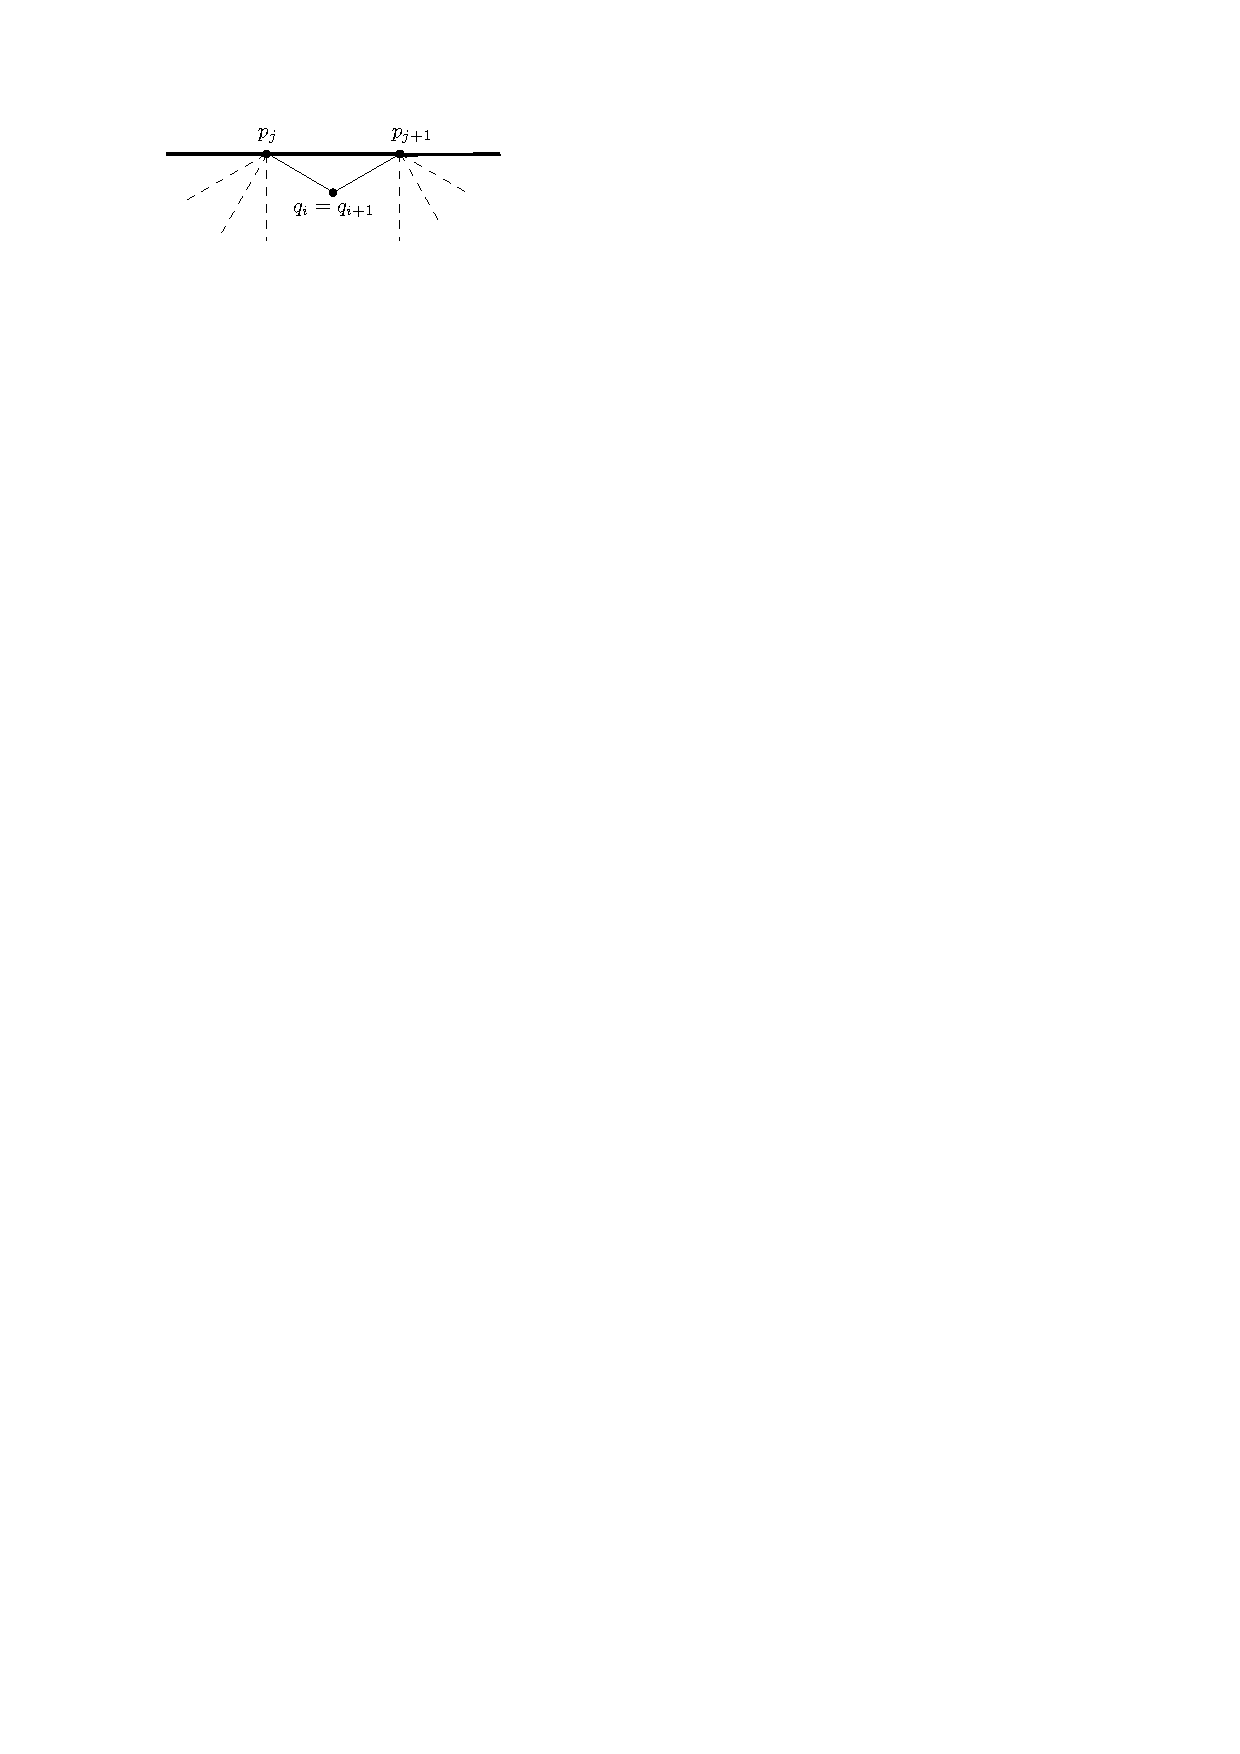
\includegraphics[width=\linewidth]{unifiedAlgo/img/walkProofB}
\clearpage% page: 19
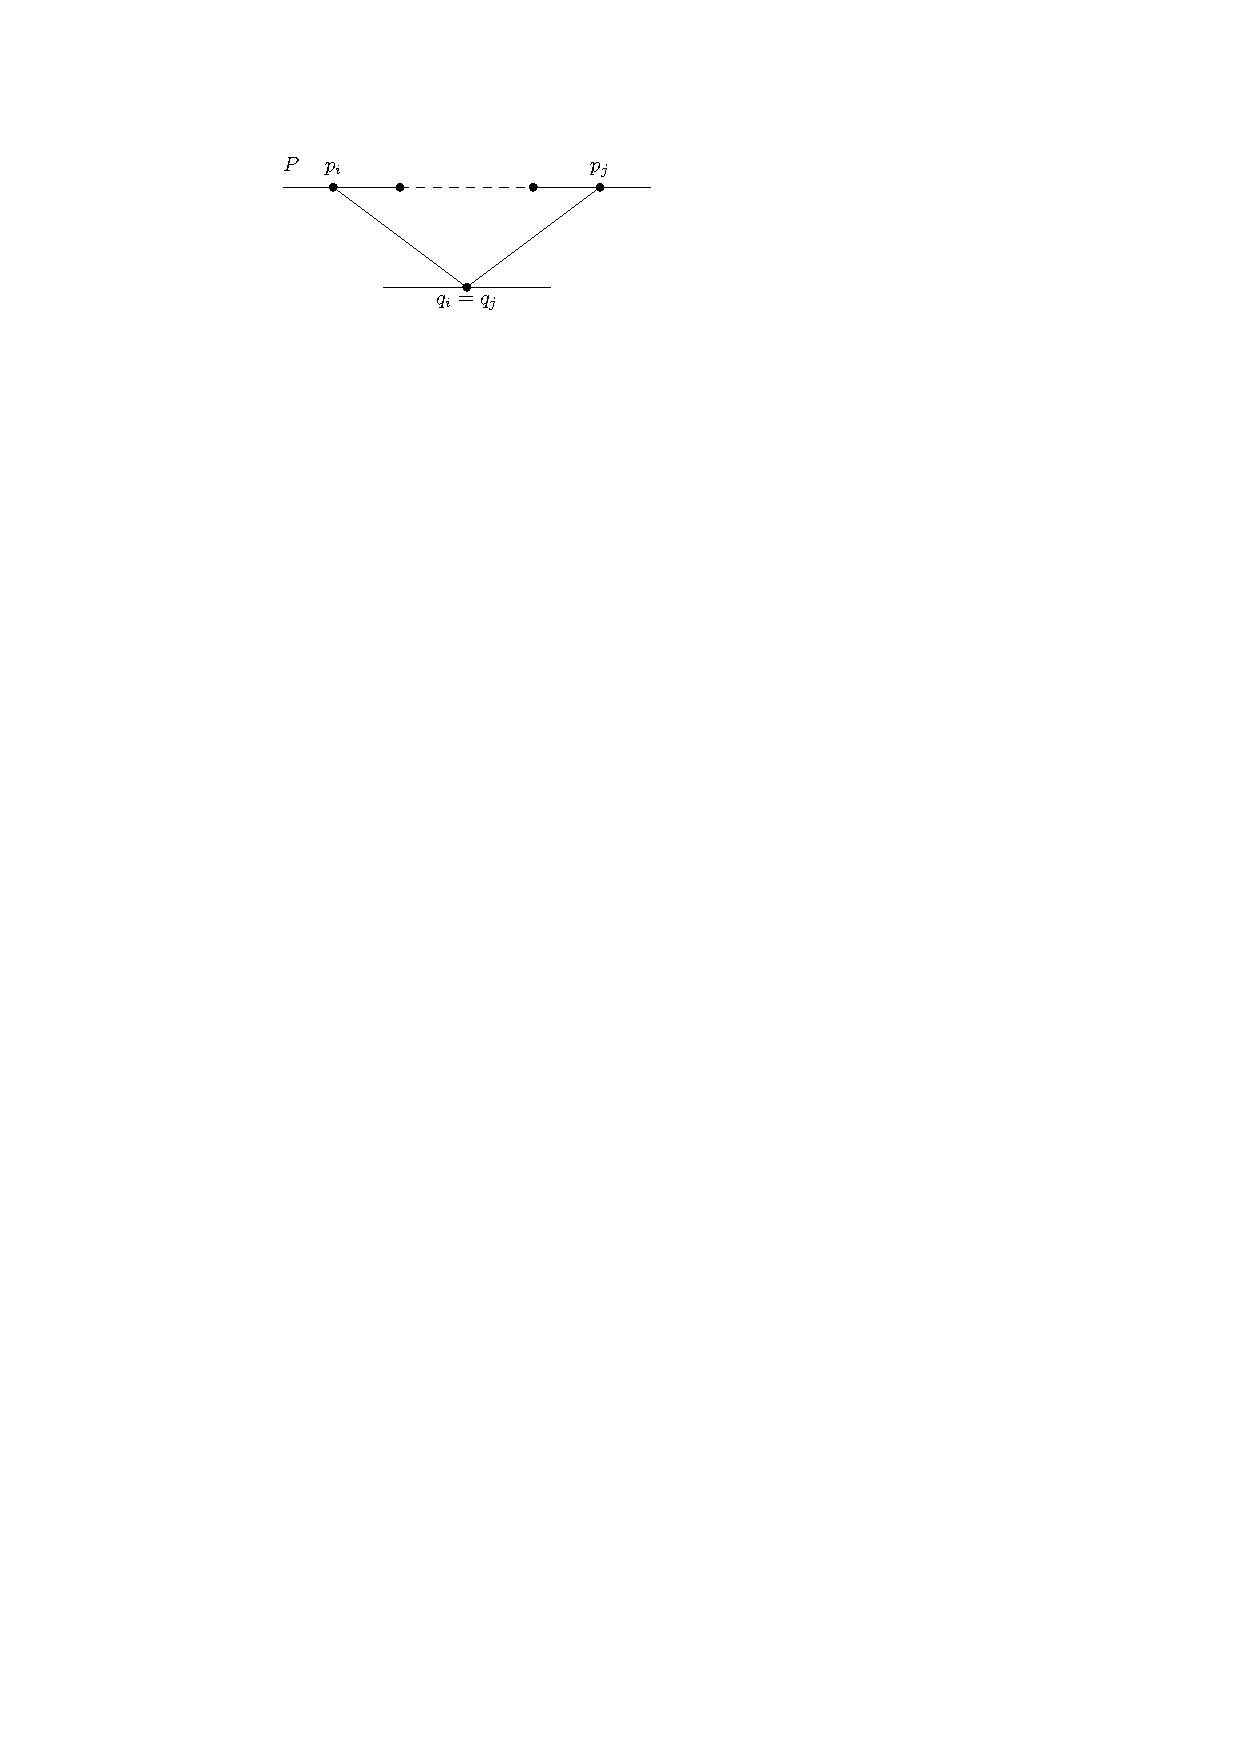
\includegraphics[scale=1]{./unifiedAlgo/img/rightNeighbourwalk/neighborPathisPath.pdf}
\clearpage% page: 20
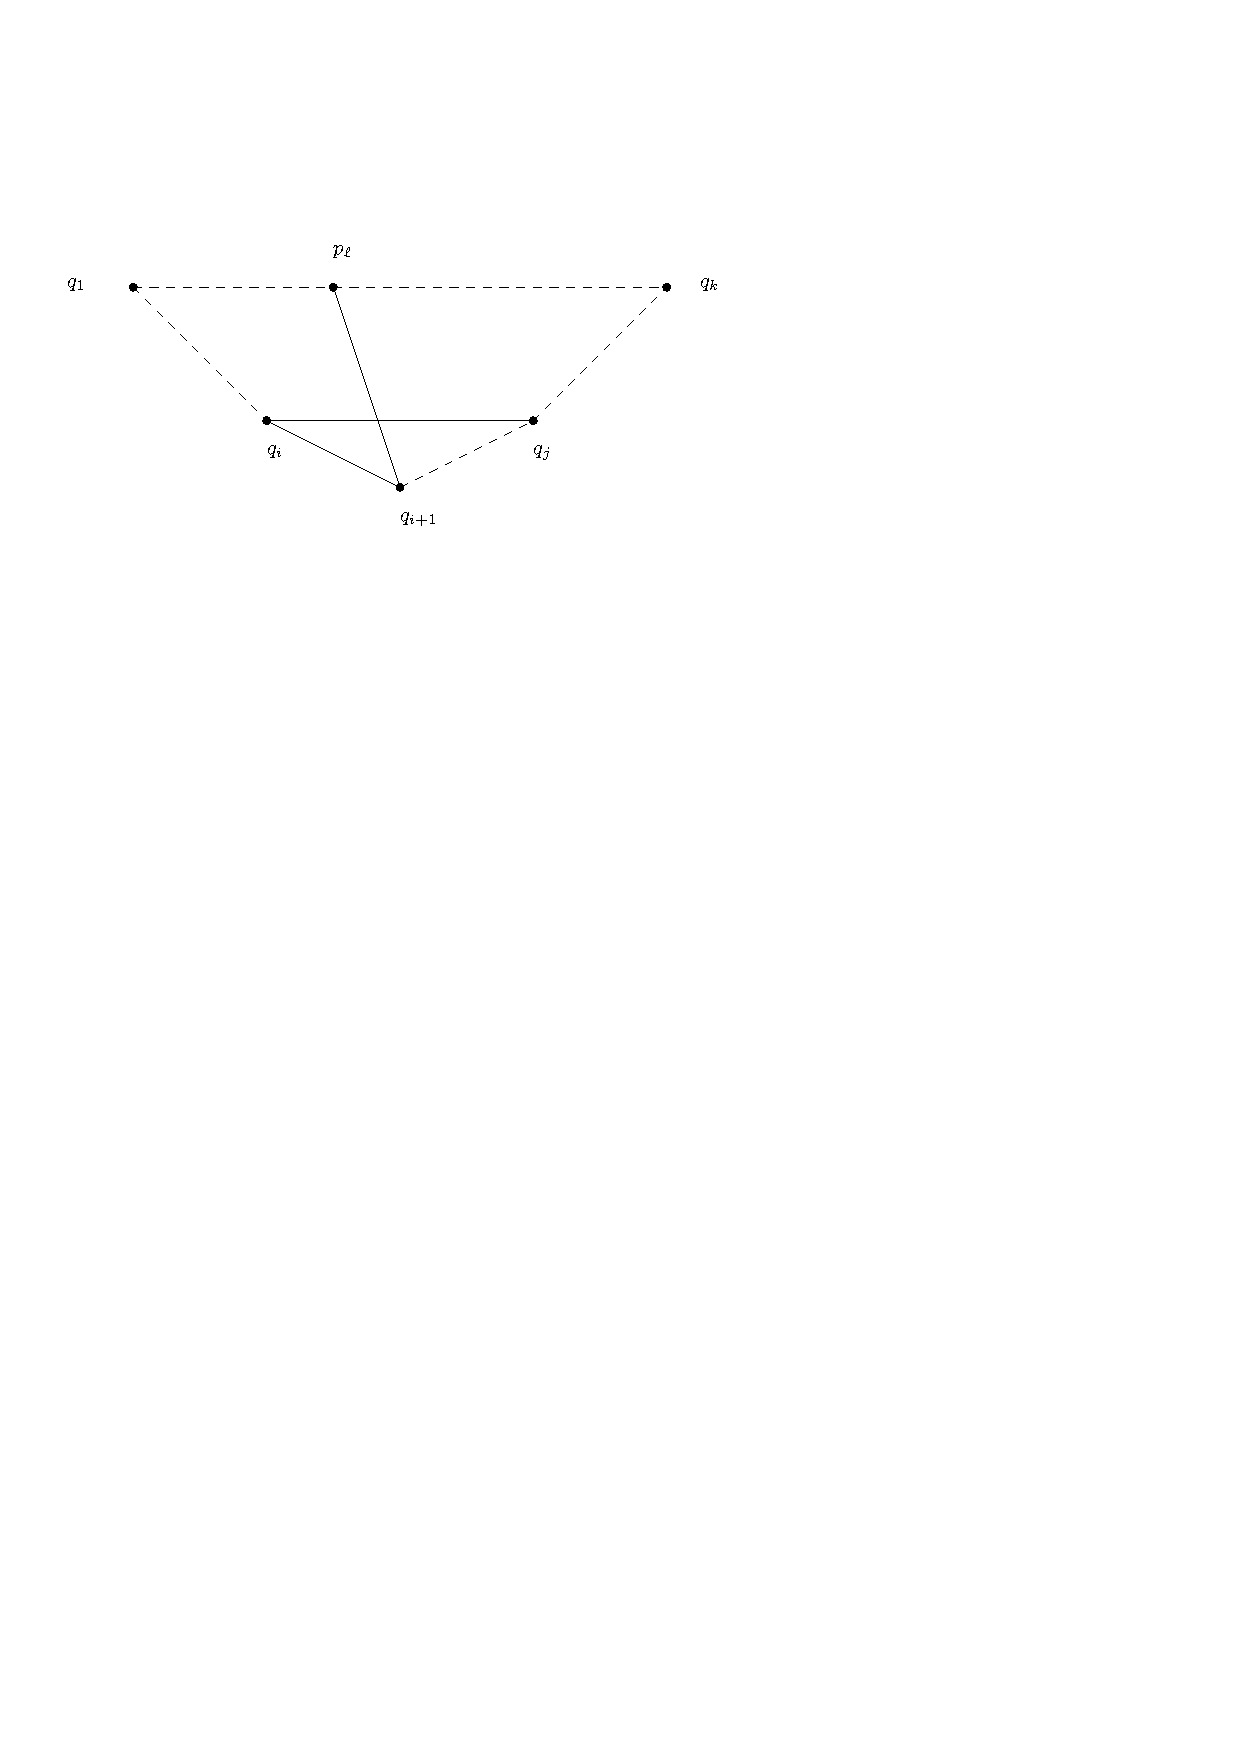
\includegraphics[scale=1]{unifiedAlgo/img/rightNeighbourwalk/neighbourWalkChords}
\clearpage% page: 21
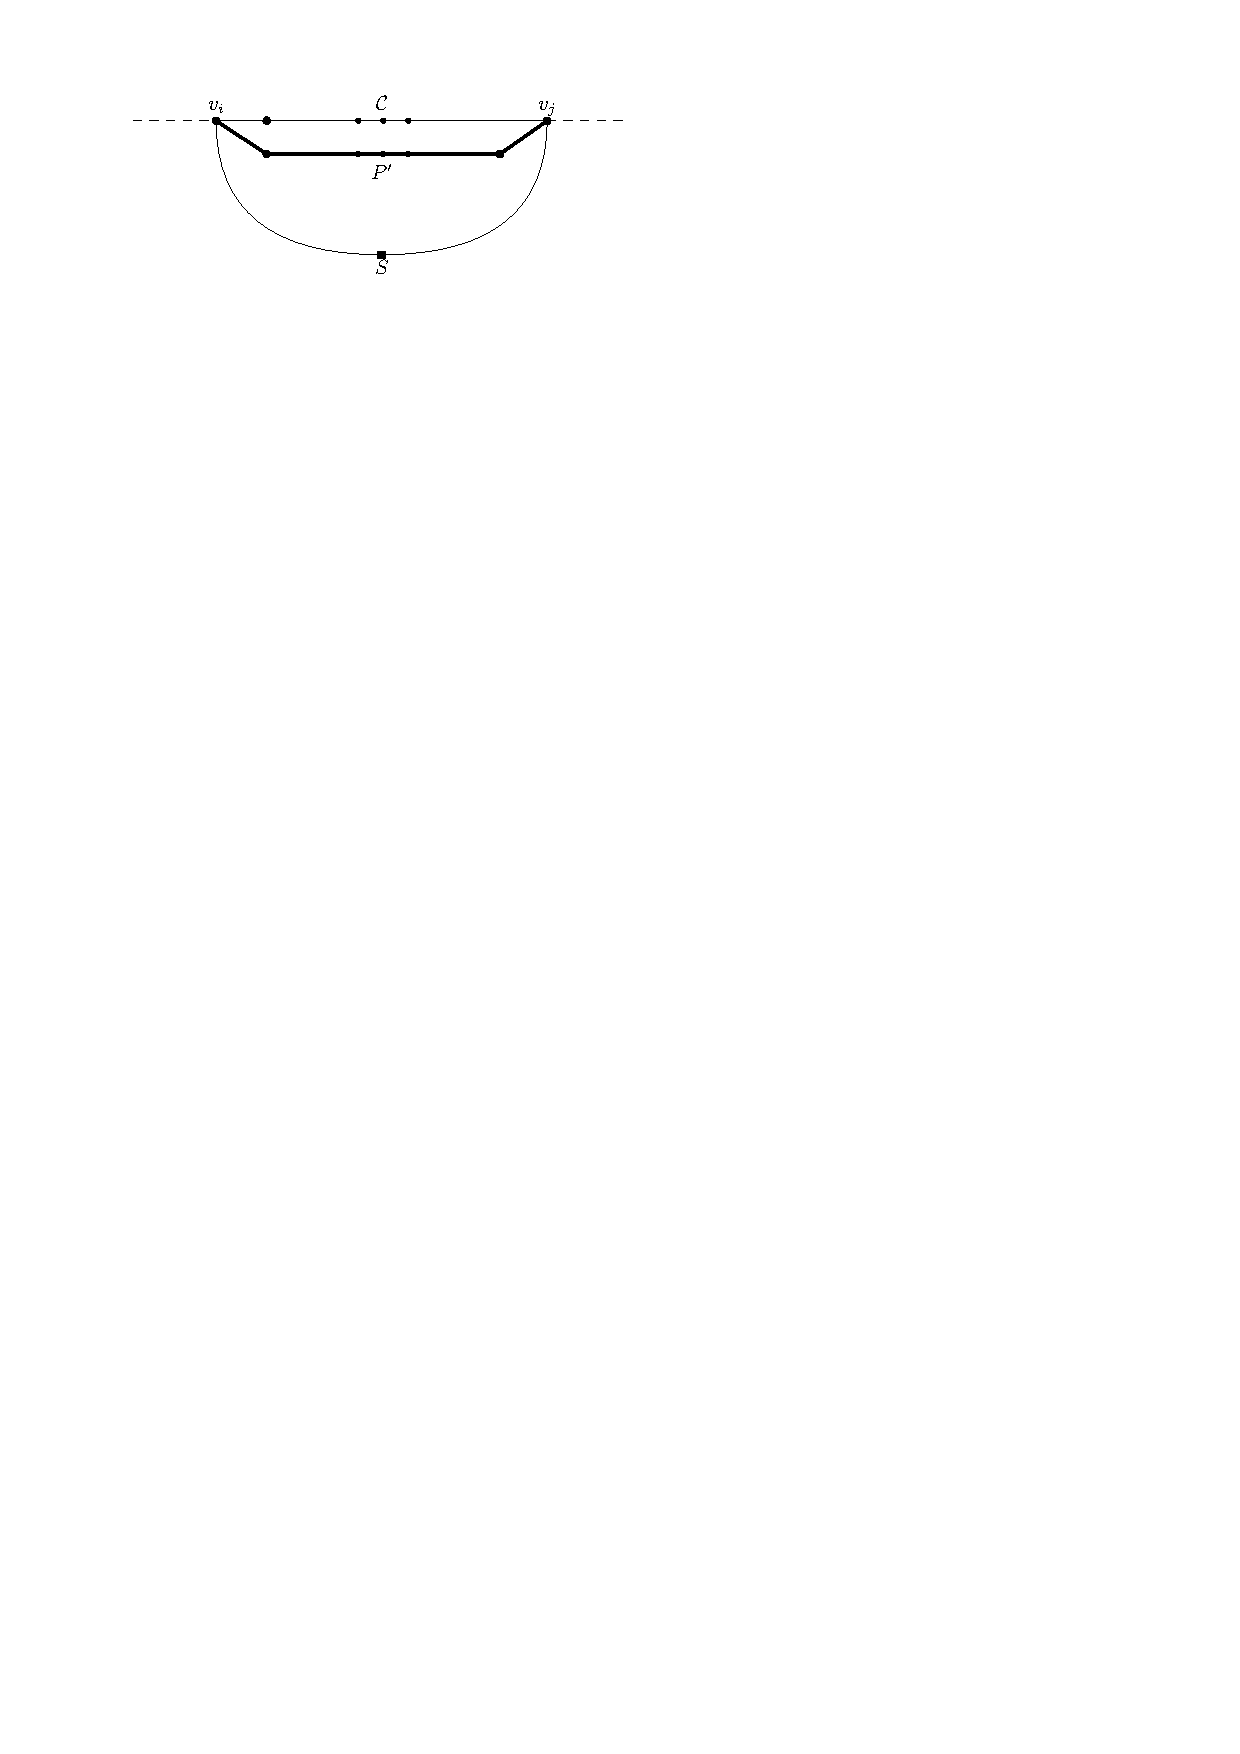
\includegraphics[scale=1]{unifiedAlgo/img/sweep/cases/noIrregularity}
\clearpage% page: 22
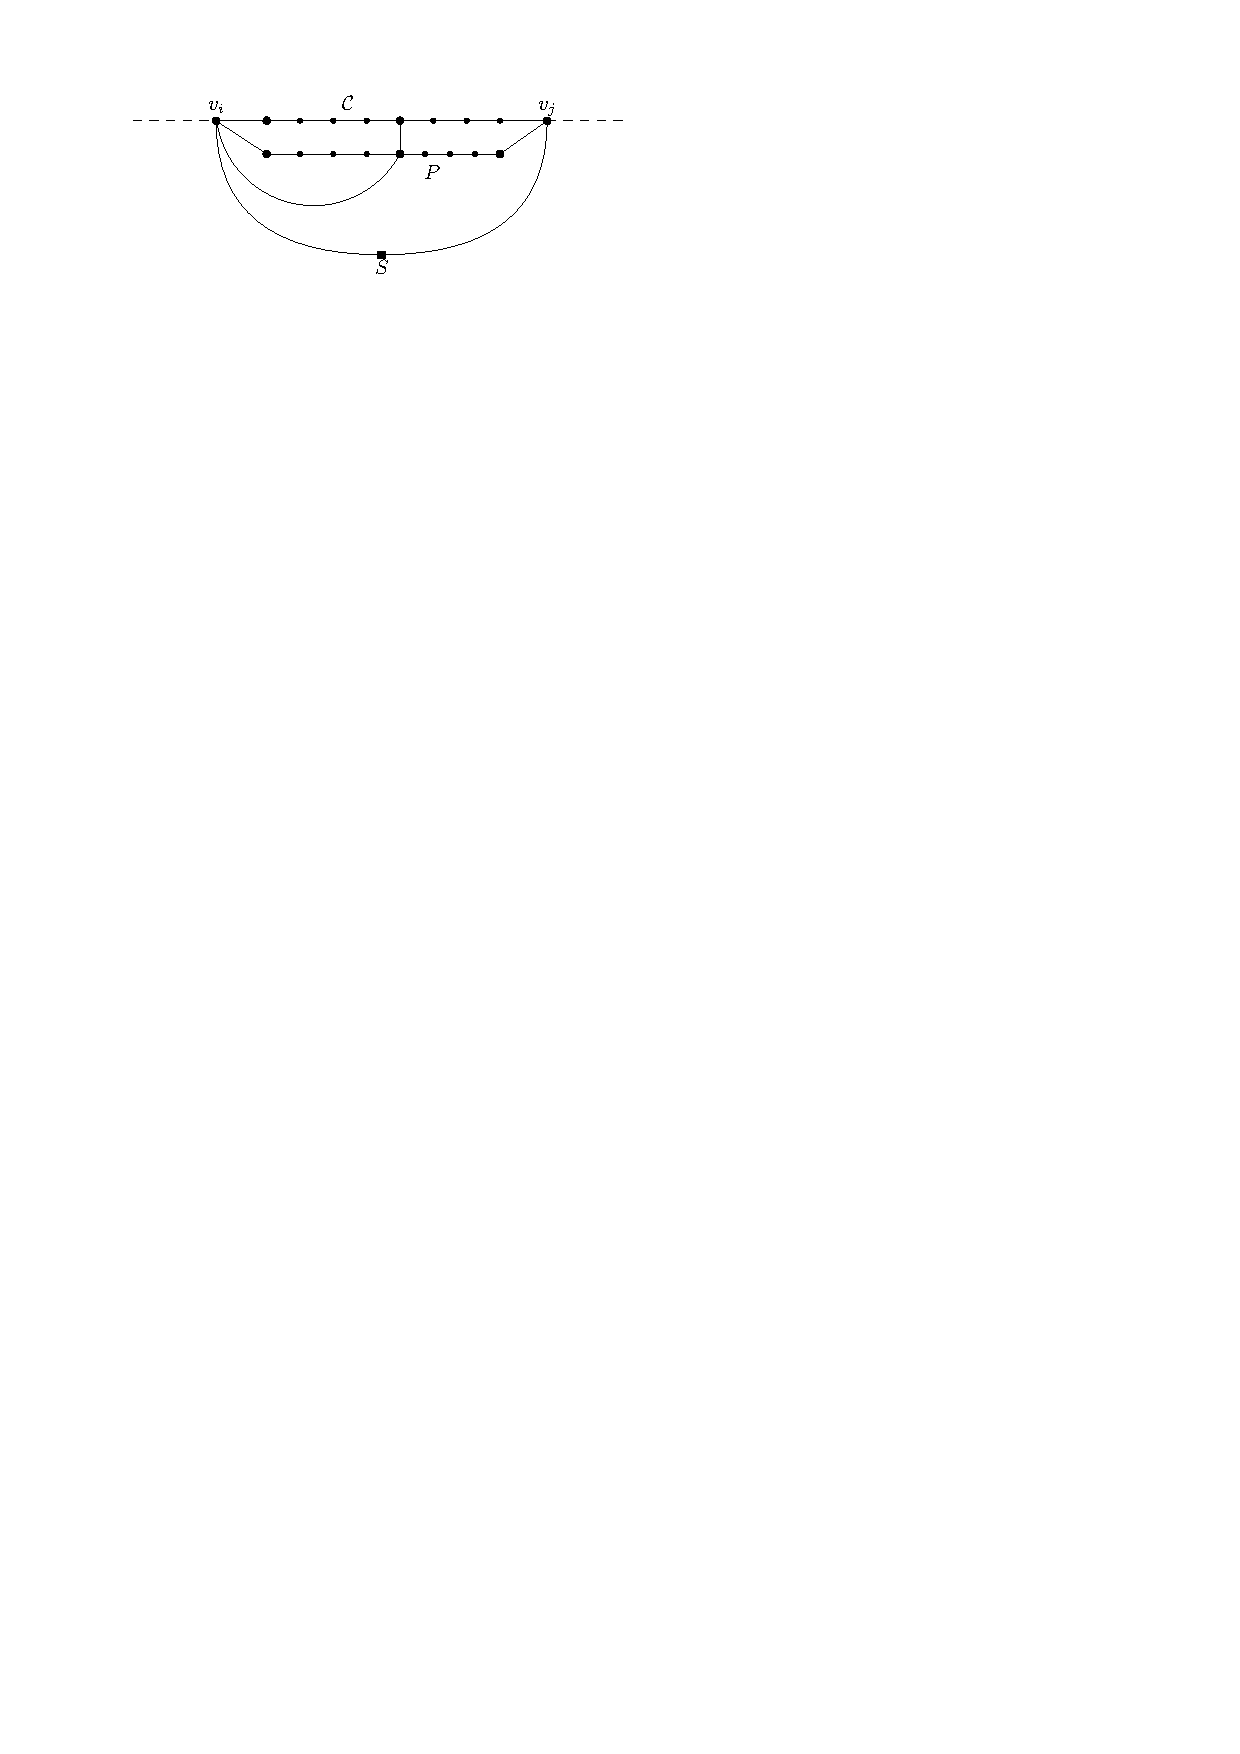
\includegraphics[scale=1]{./unifiedAlgo/img/sweep/noChordOnExtriorVertex.pdf}
\clearpage% page: 23
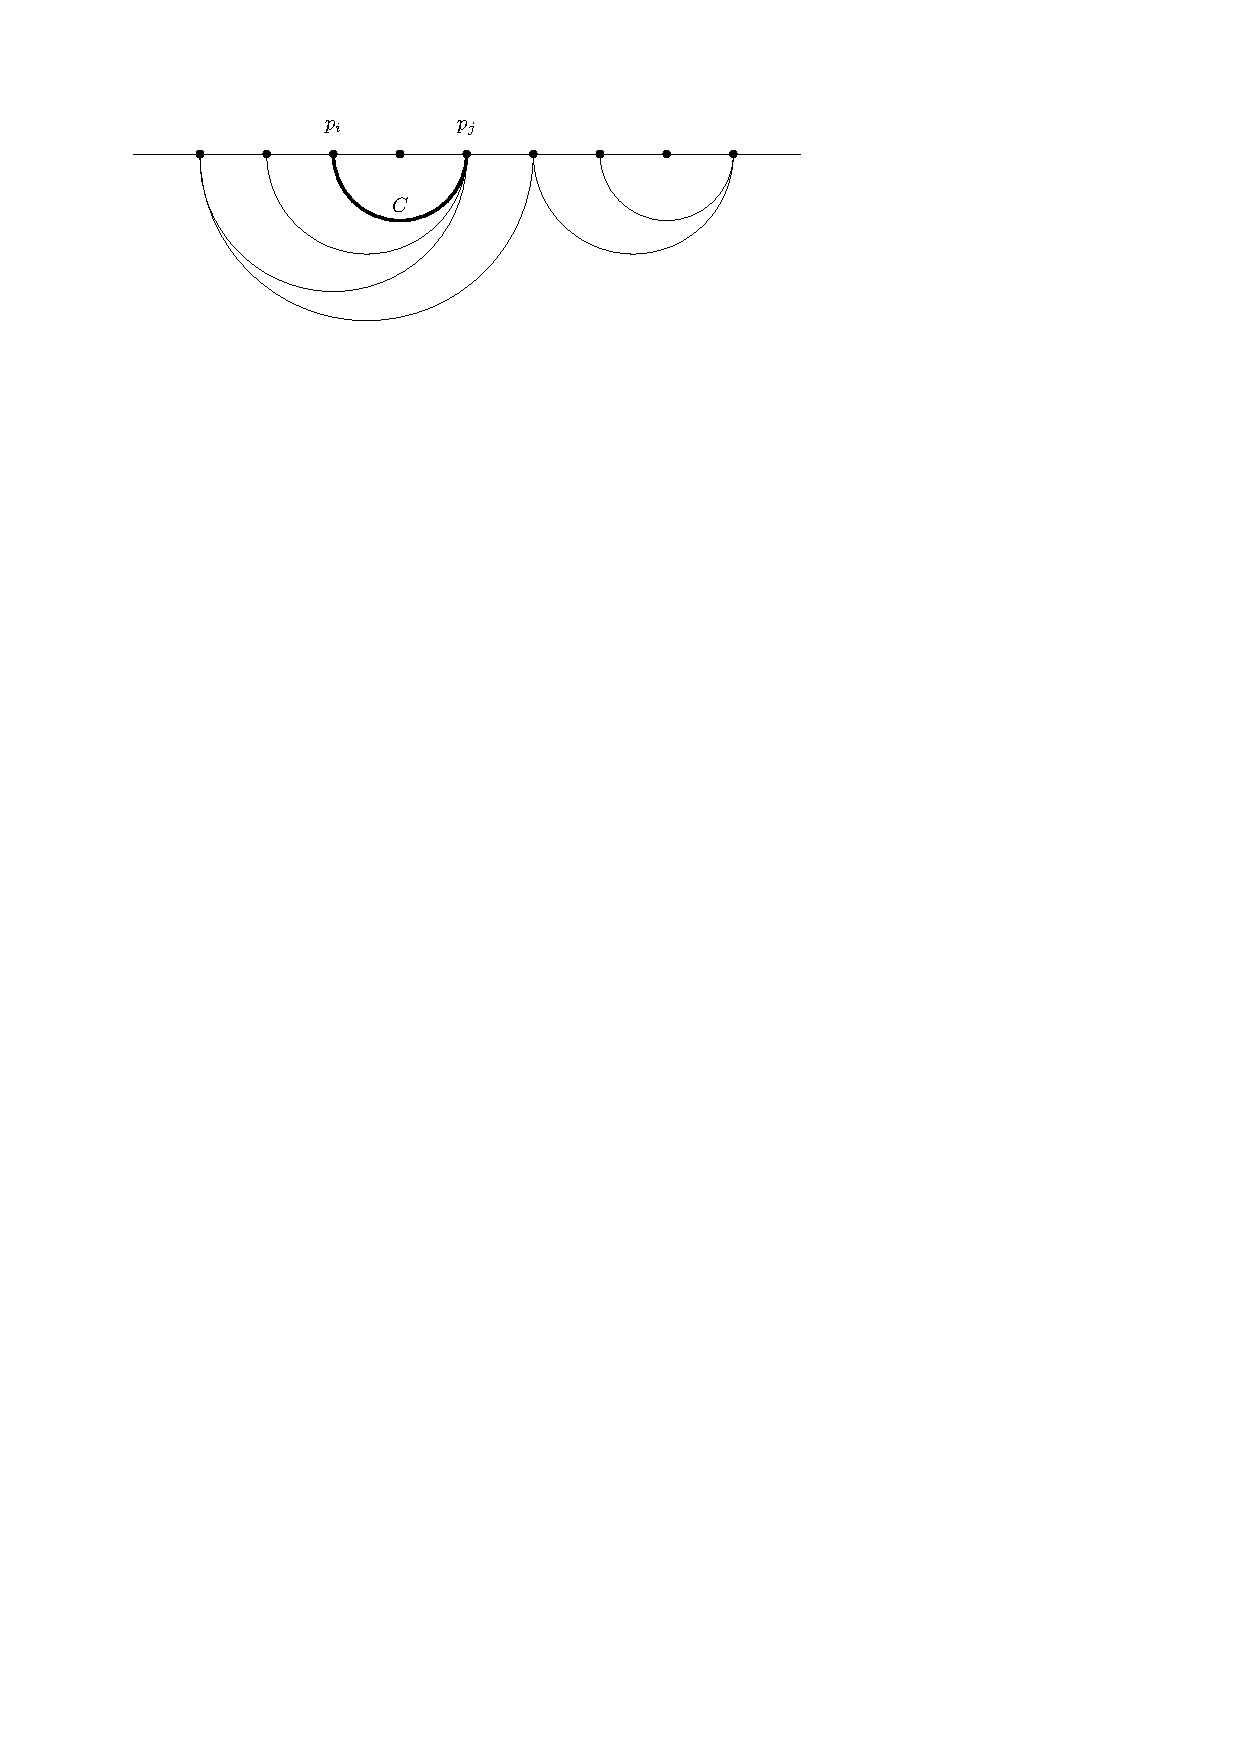
\includegraphics[scale=1]{unifiedalgo/img/sweep/chordsOnCandidatePath}
\clearpage% page: 24
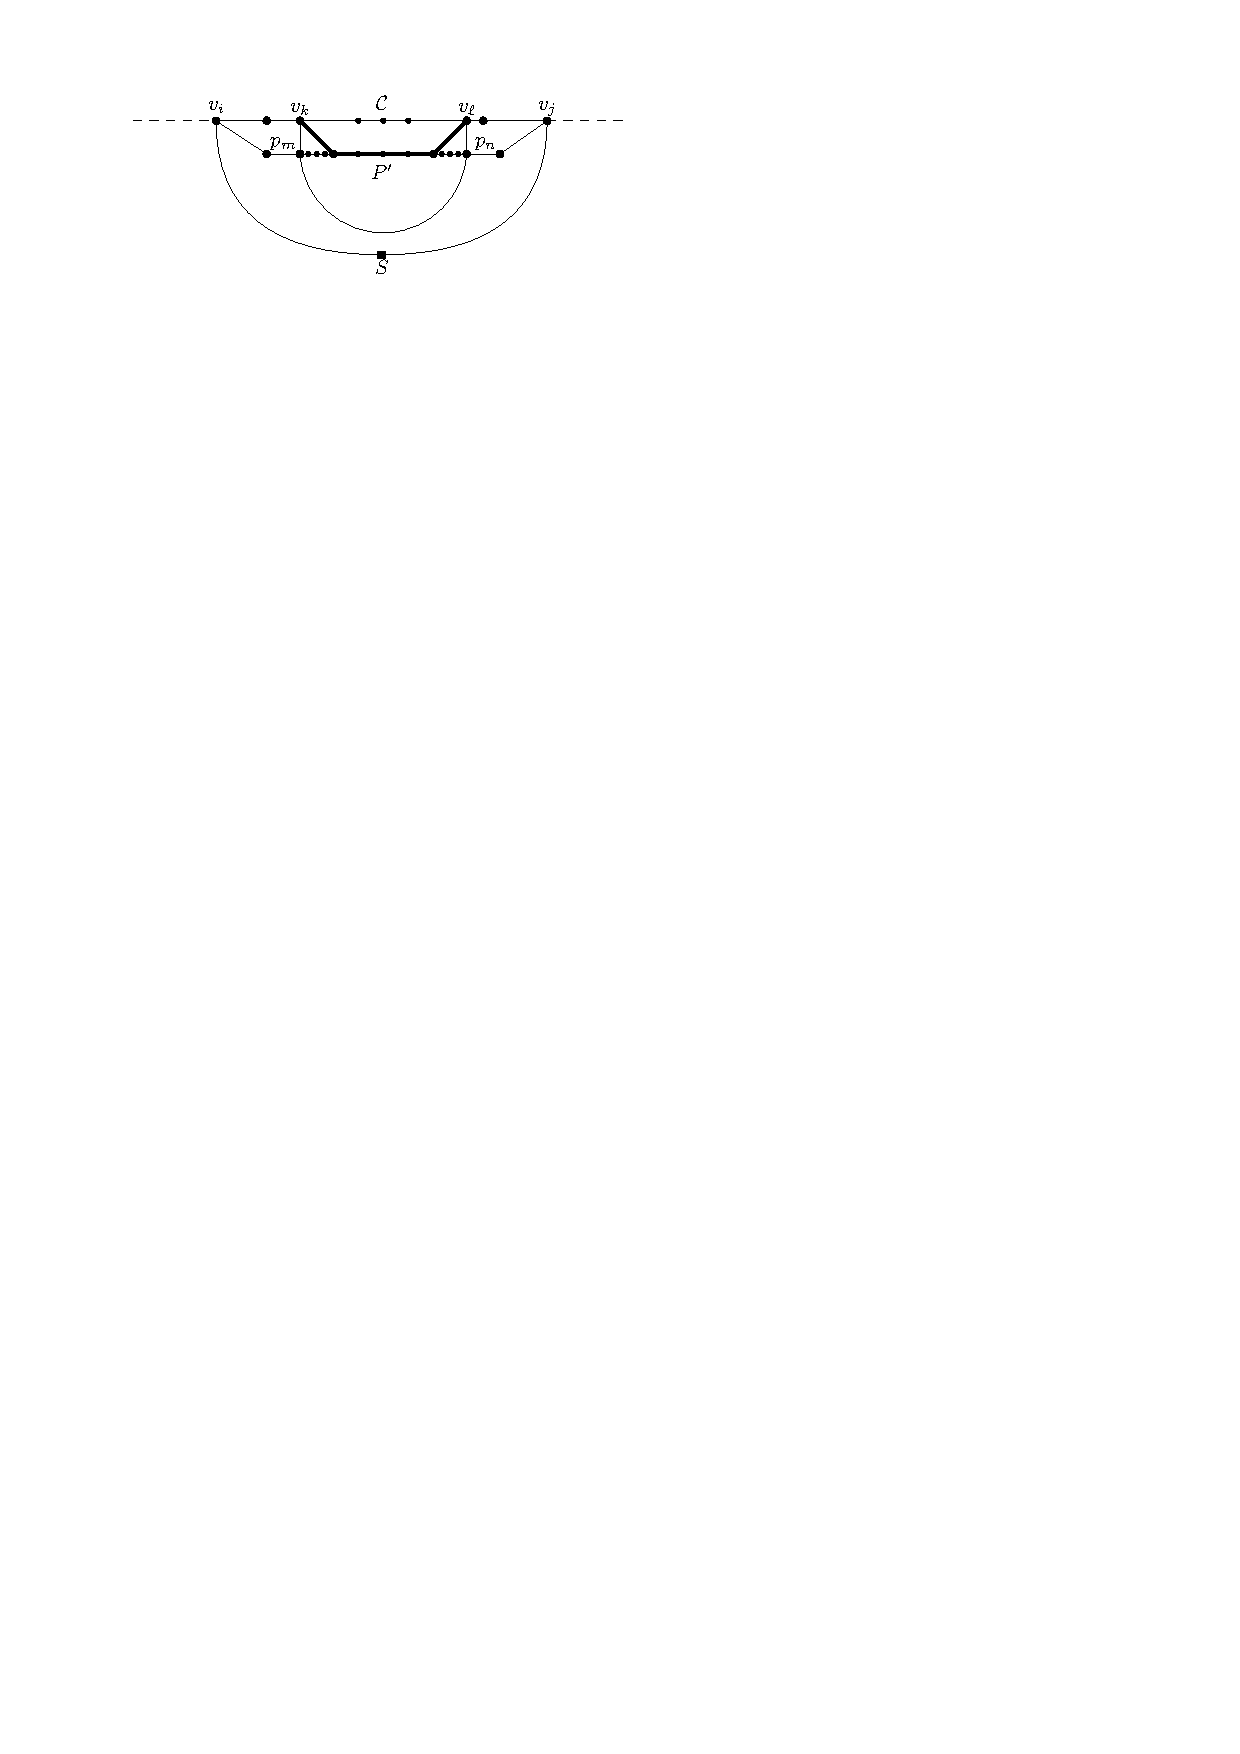
\includegraphics[scale=1]{unifiedAlgo/img/sweep/cases/chordUpdate}
\clearpage% page: 25
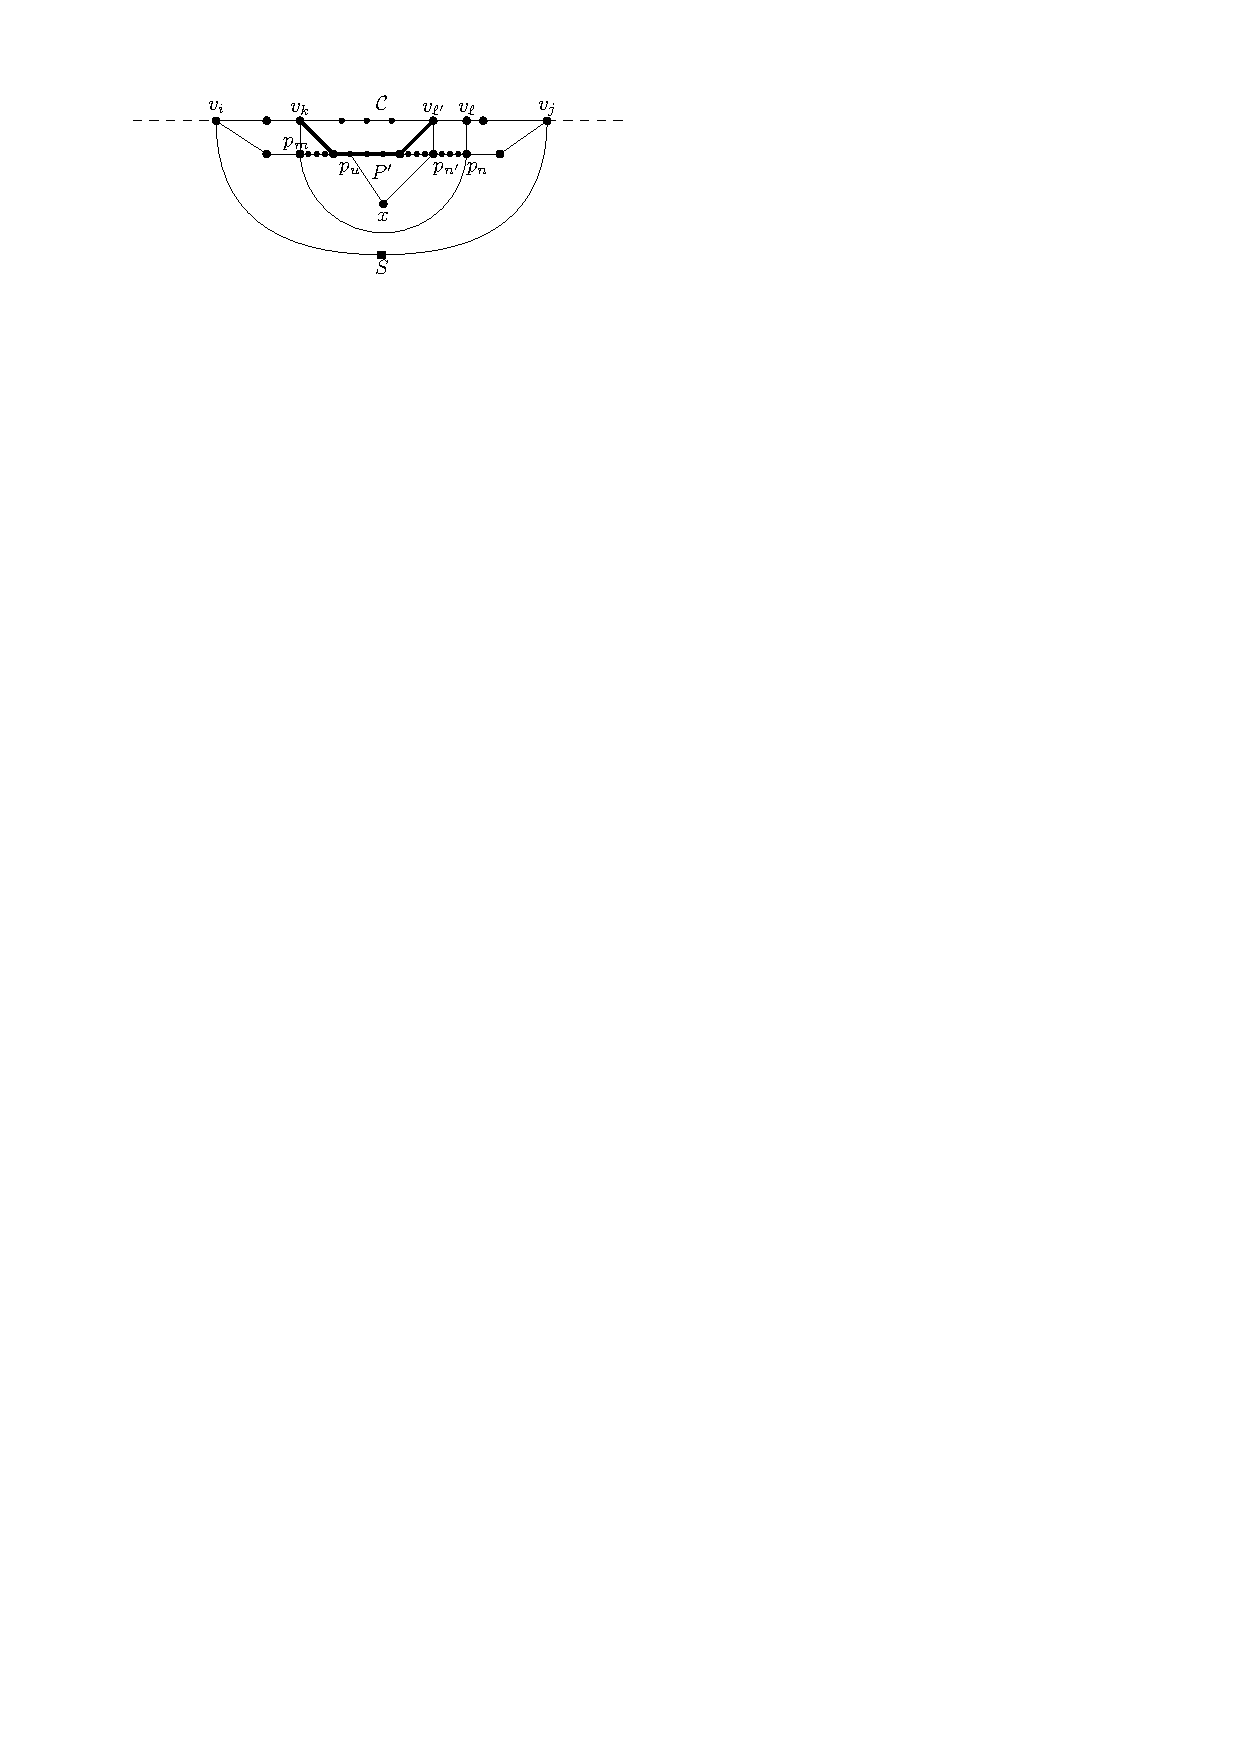
\includegraphics[scale=1]{unifiedAlgo/img/sweep/cases/2chordInChordUpdate}
\clearpage% page: 26
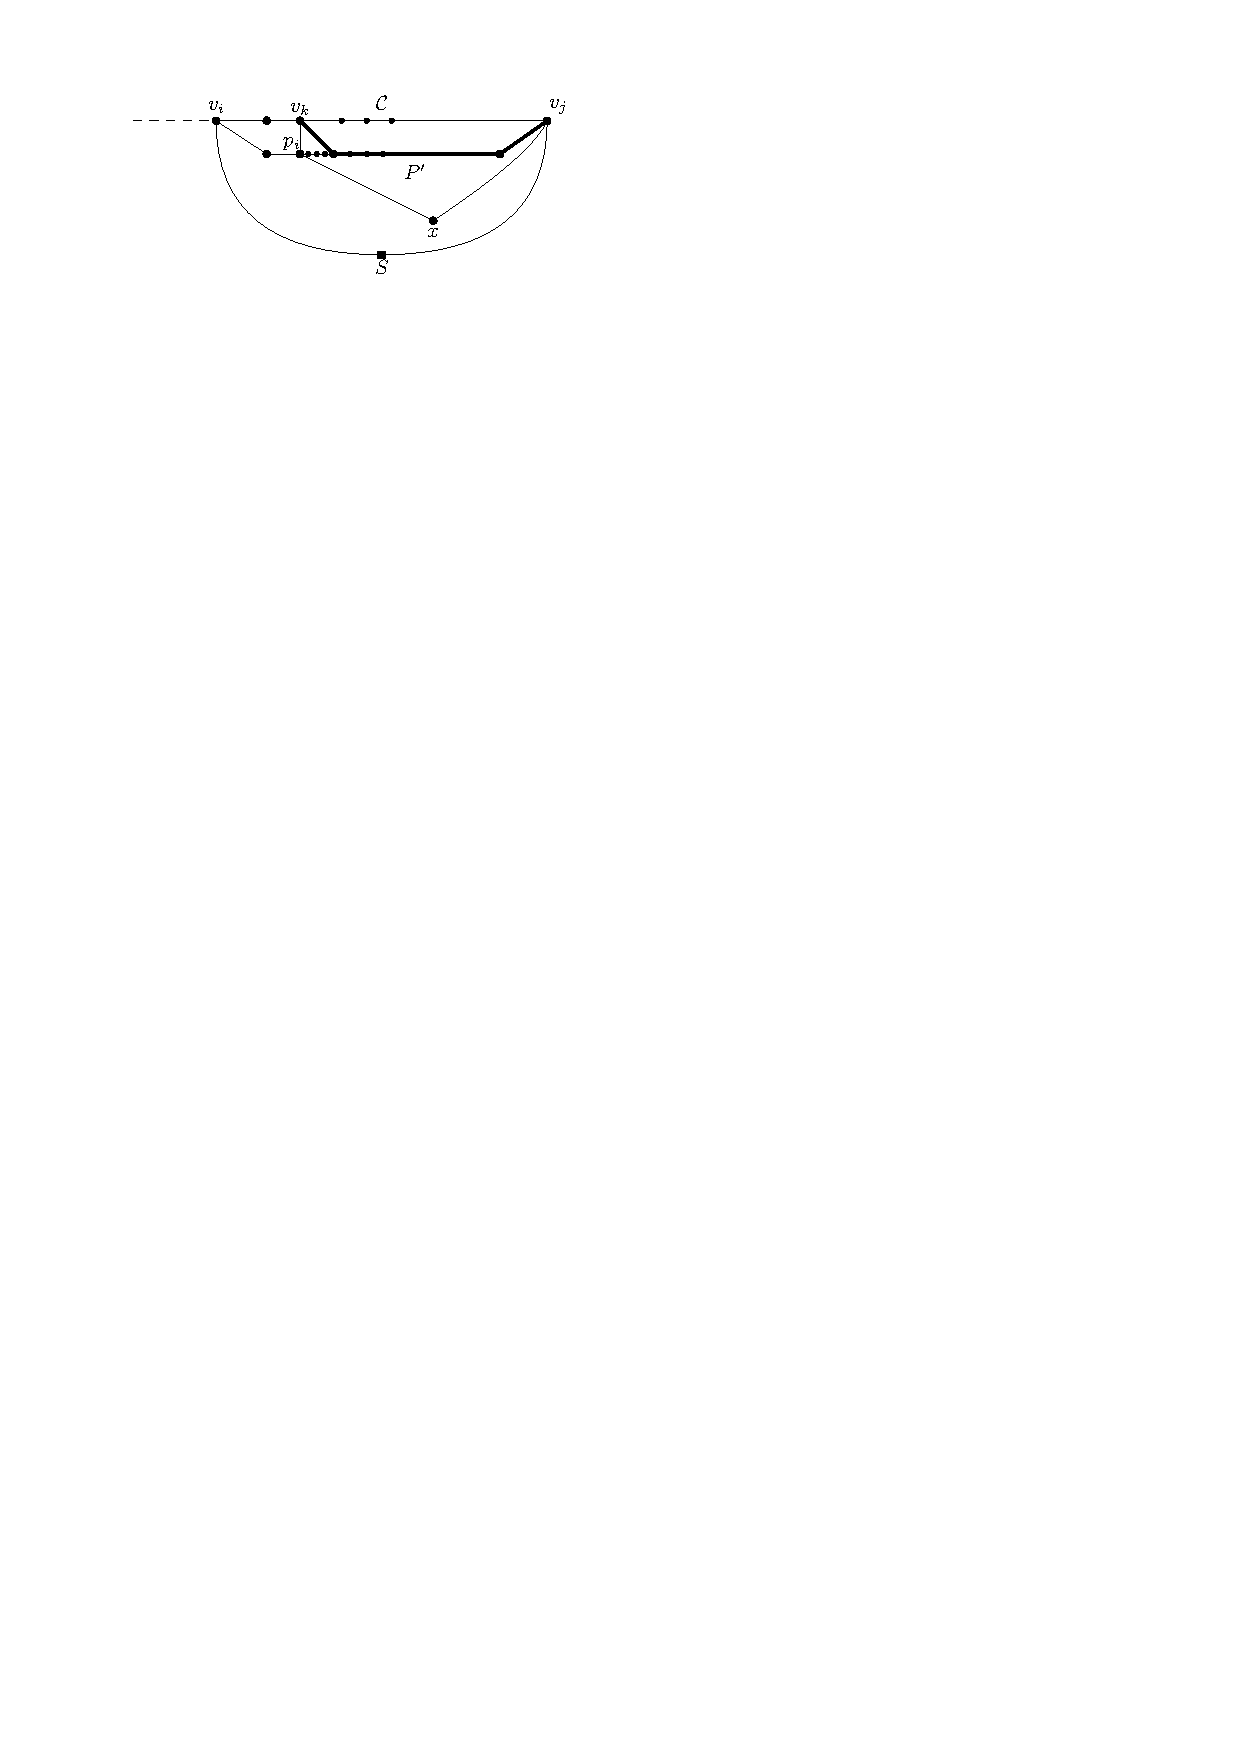
\includegraphics[scale=1]{unifiedAlgo/img/sweep/cases/pEBound}
\clearpage% page: 27
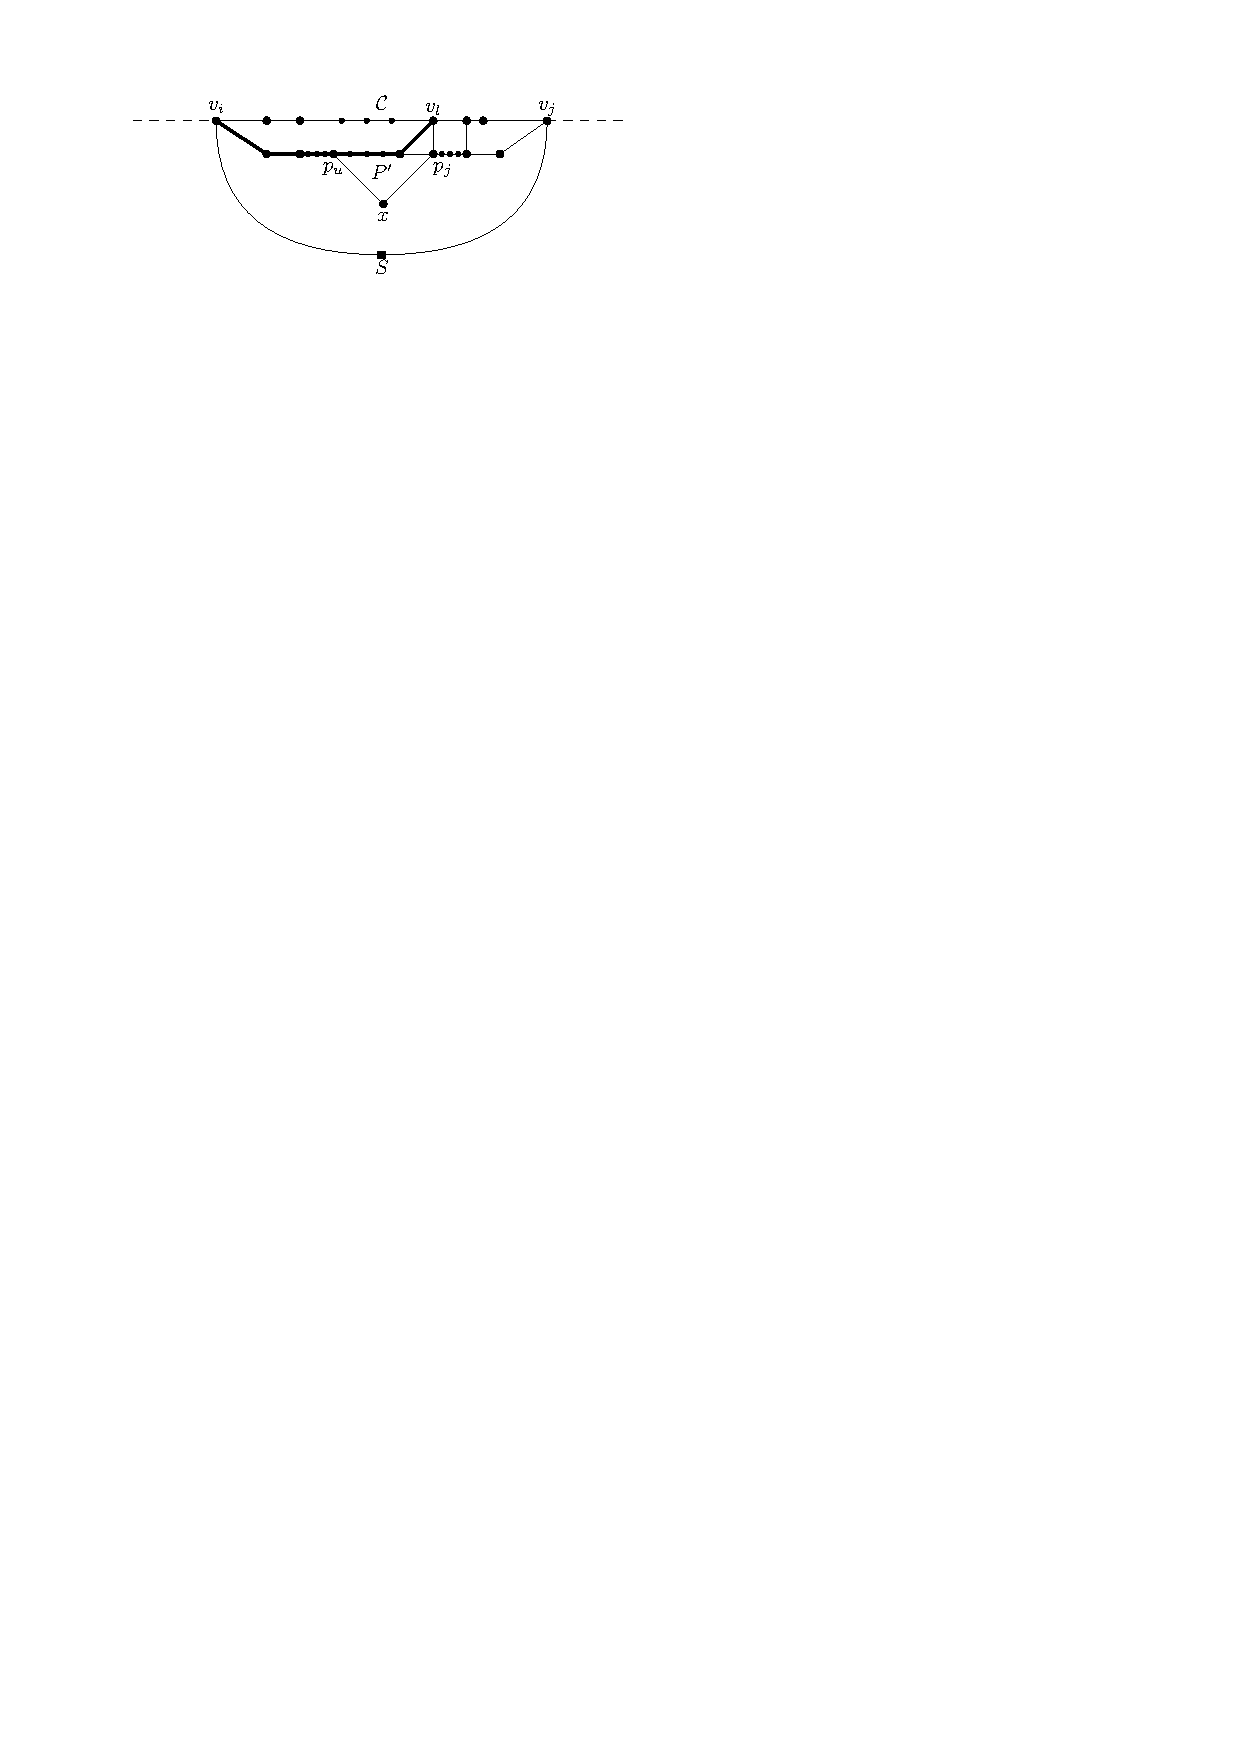
\includegraphics[scale=1]{unifiedAlgo/img/sweep/cases/free2chord}
\clearpage% page: 28
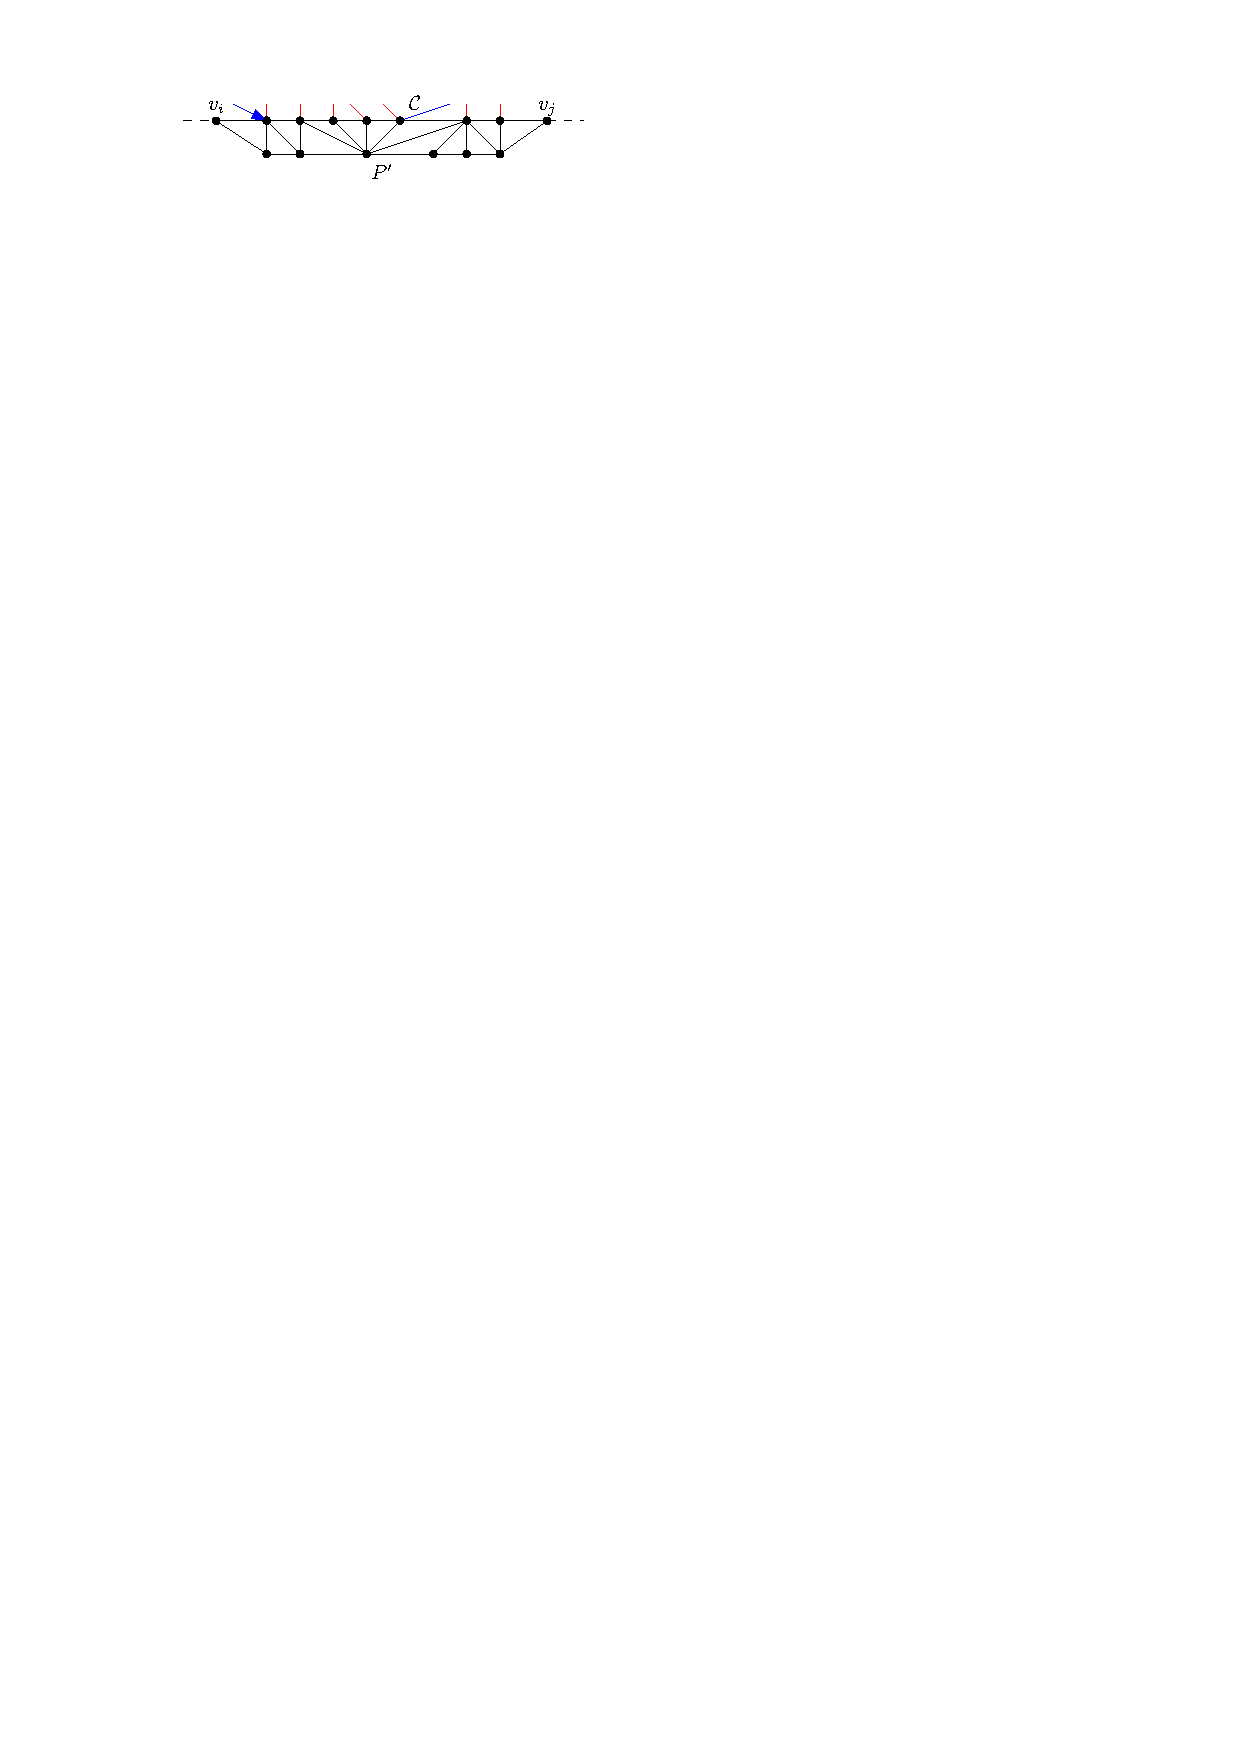
\includegraphics[width = \textwidth]{./unifiedAlgo/img/sweep/updateBefore.pdf}
\clearpage% page: 29
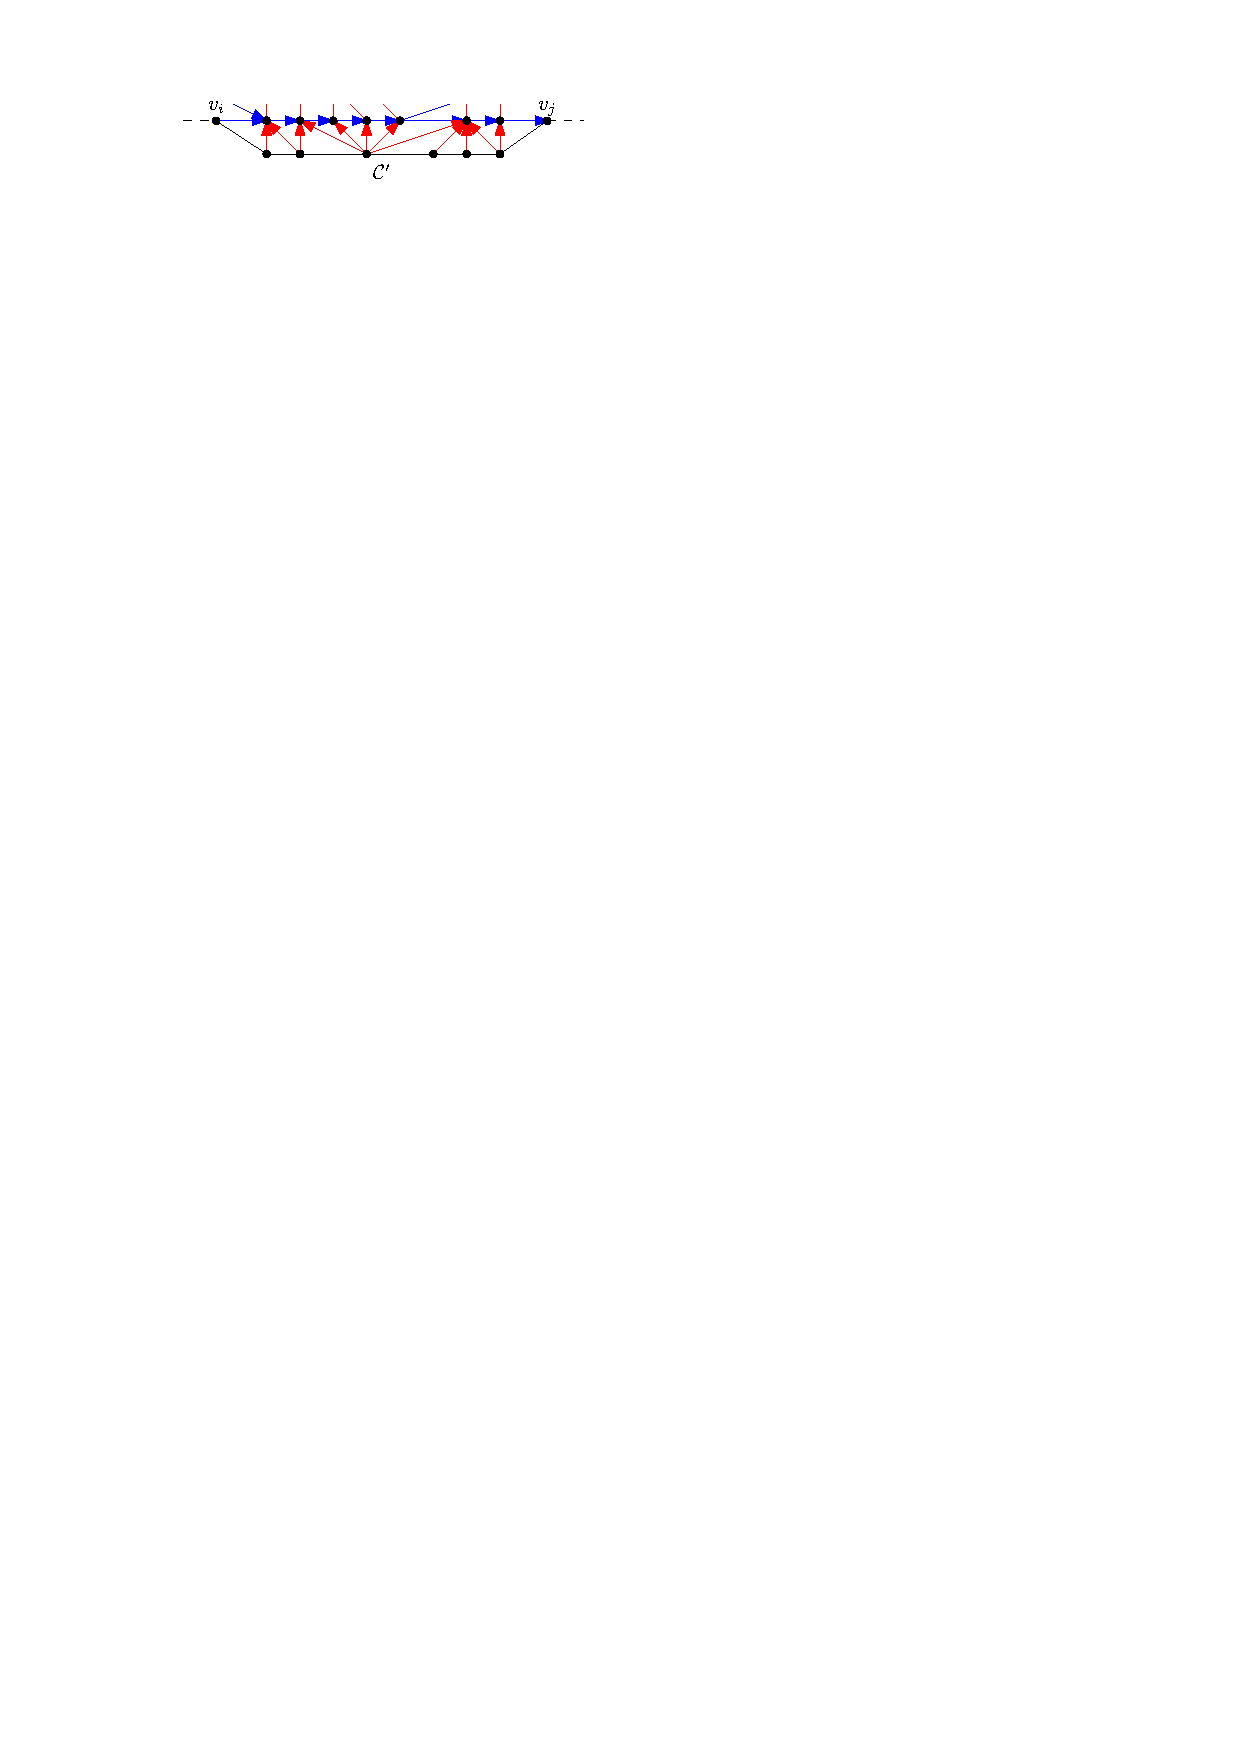
\includegraphics[width =\textwidth]{./unifiedAlgo/img/sweep/updateAfter.pdf}
\clearpage% page: 30
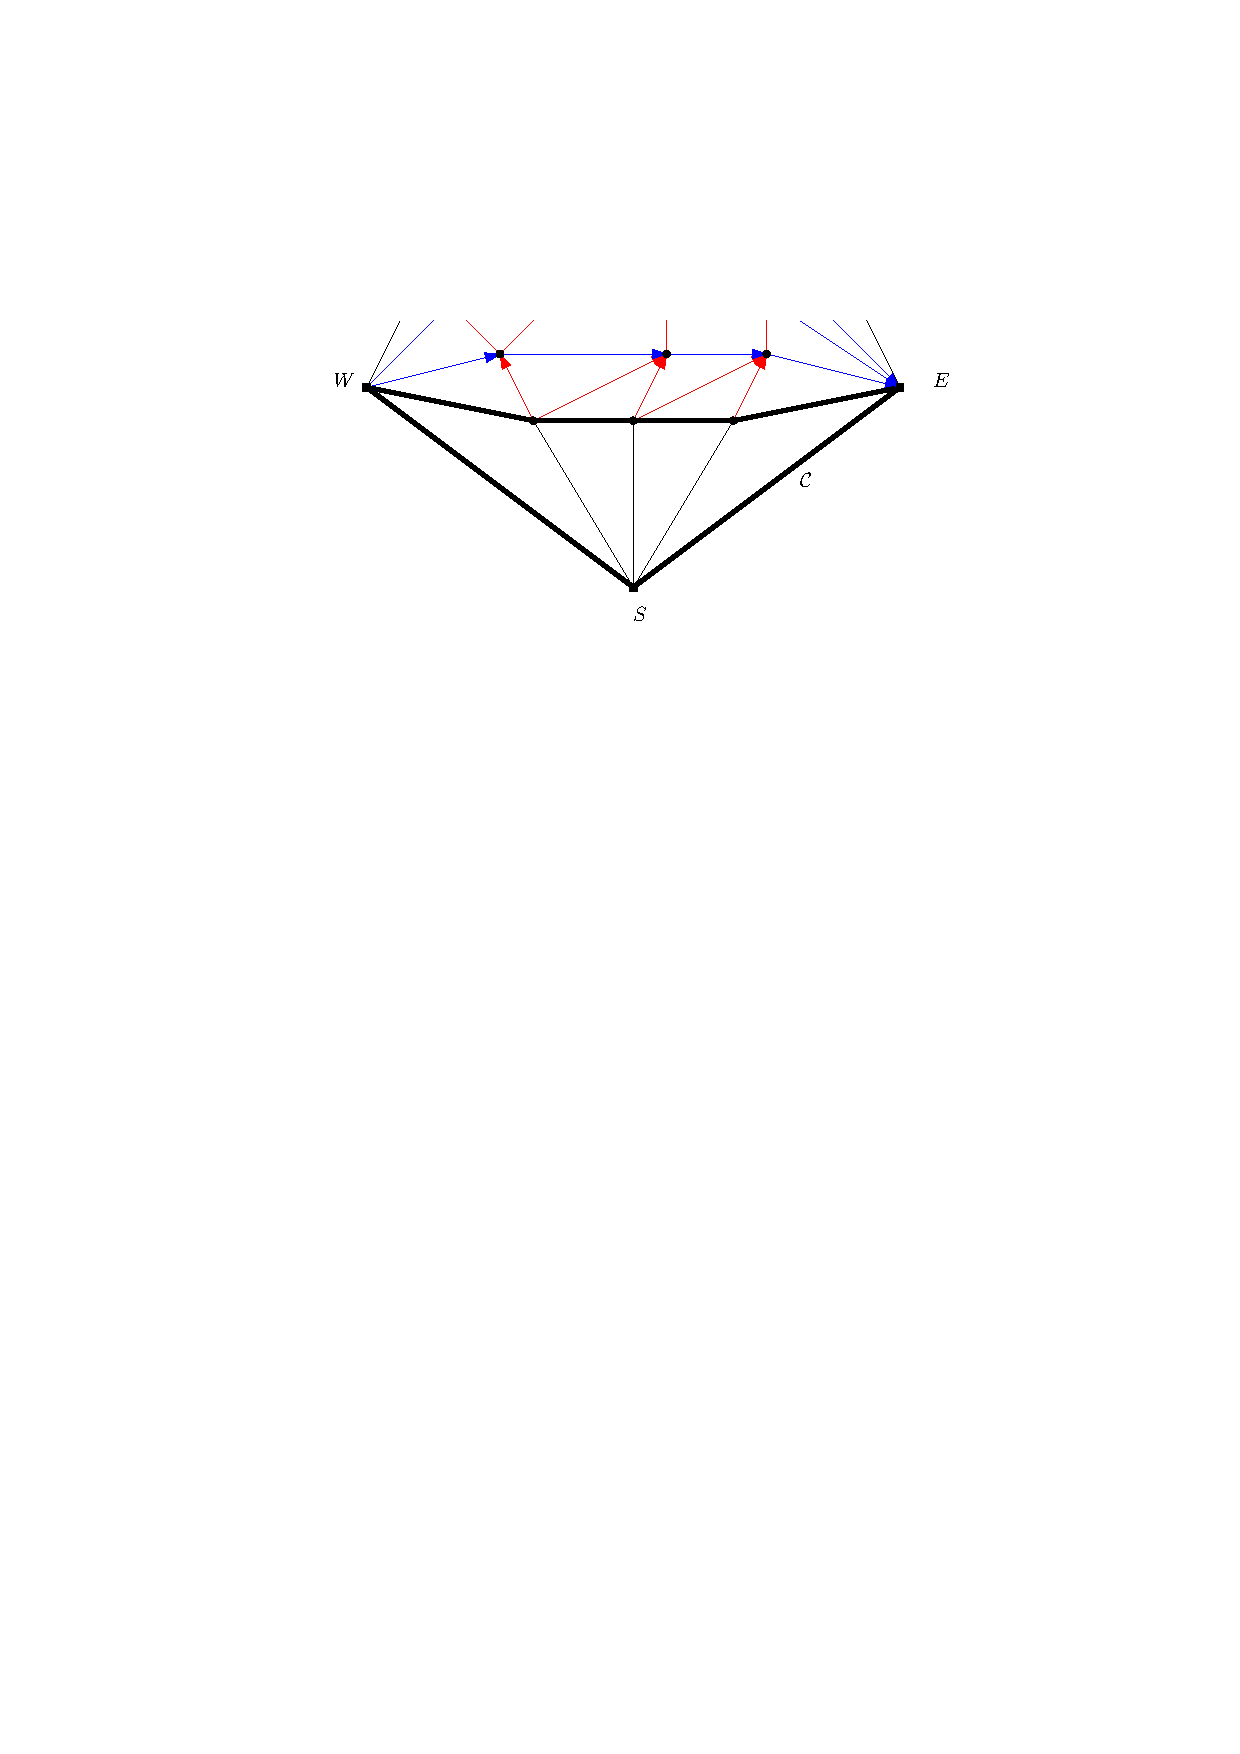
\includegraphics[width = \textwidth]{./unifiedAlgo/img/sweep/terminateBefore.pdf}
\clearpage% page: 31
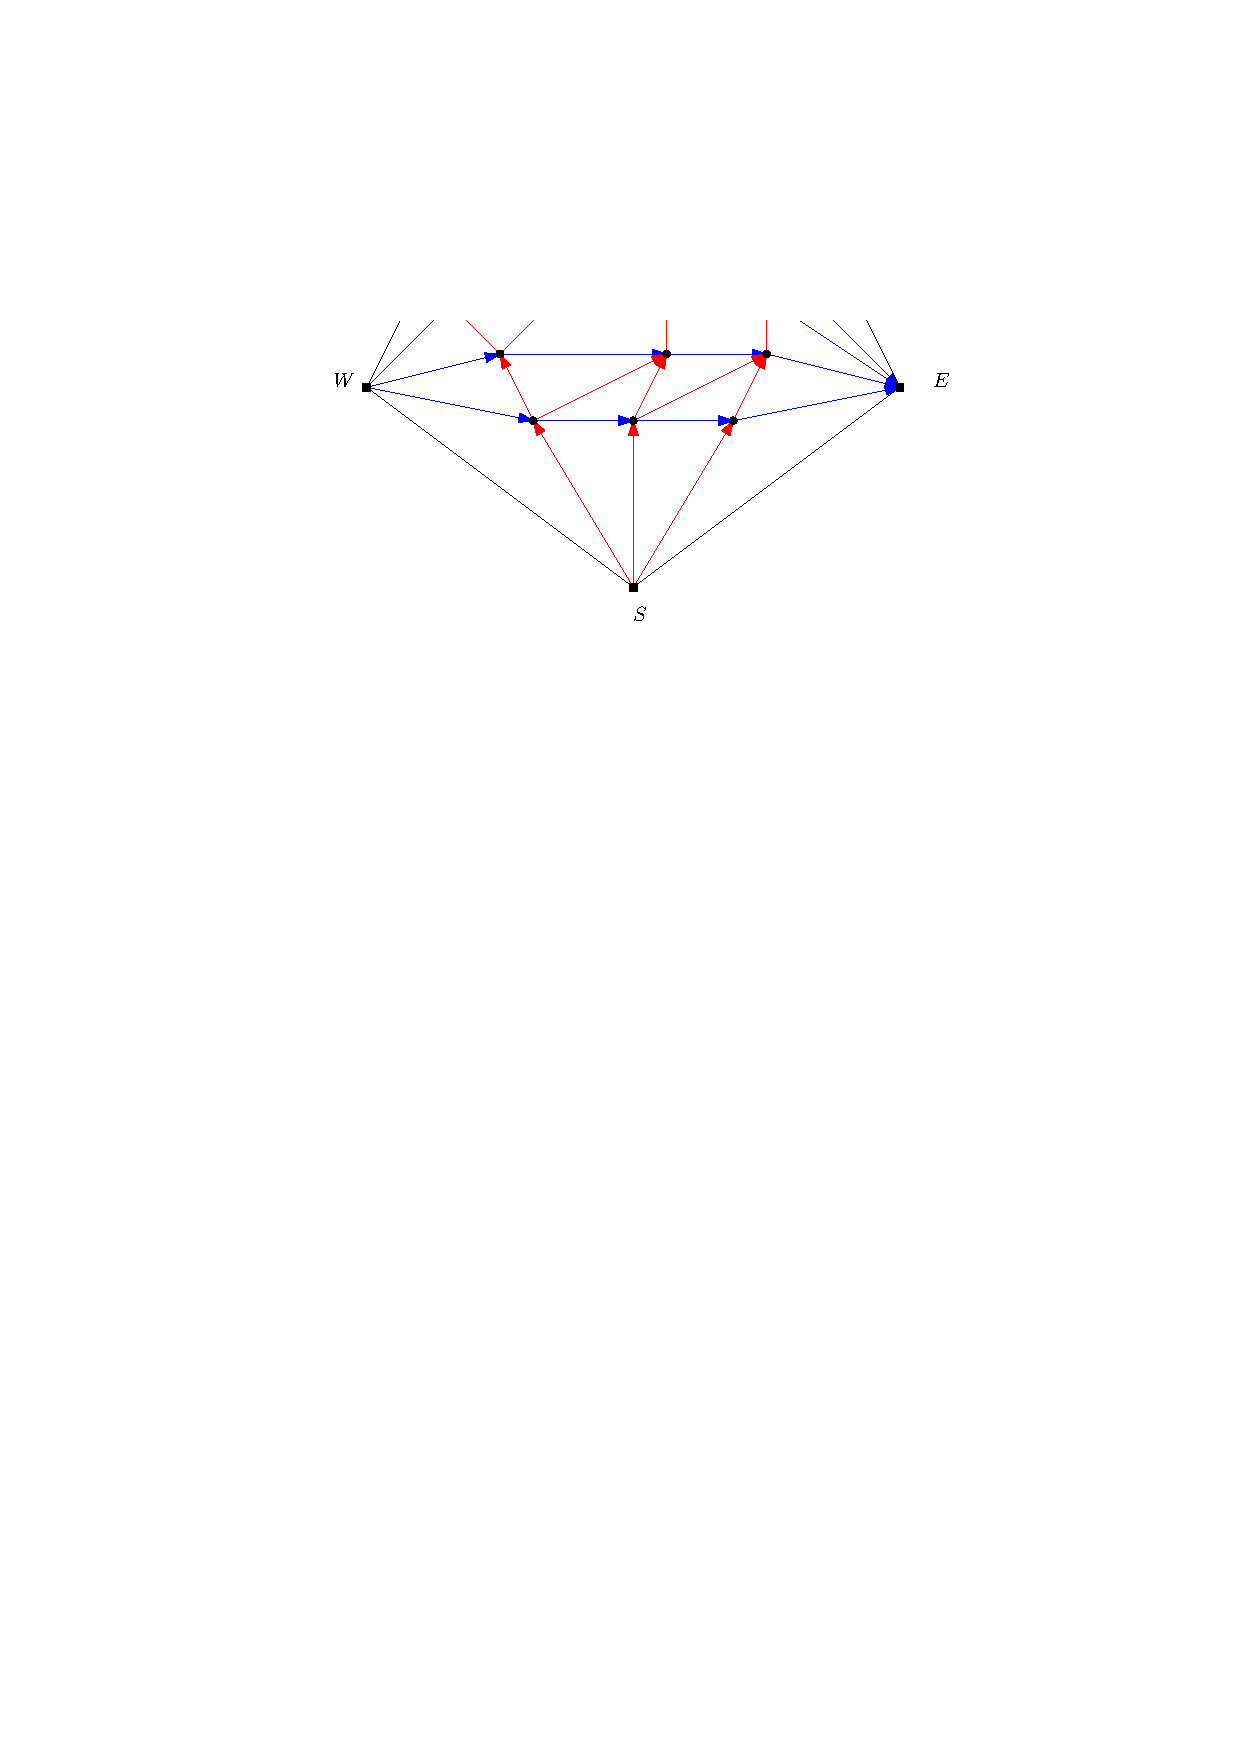
\includegraphics[width =\textwidth]{./unifiedAlgo/img/sweep/terminateAfter.pdf}
\clearpage% page: 32
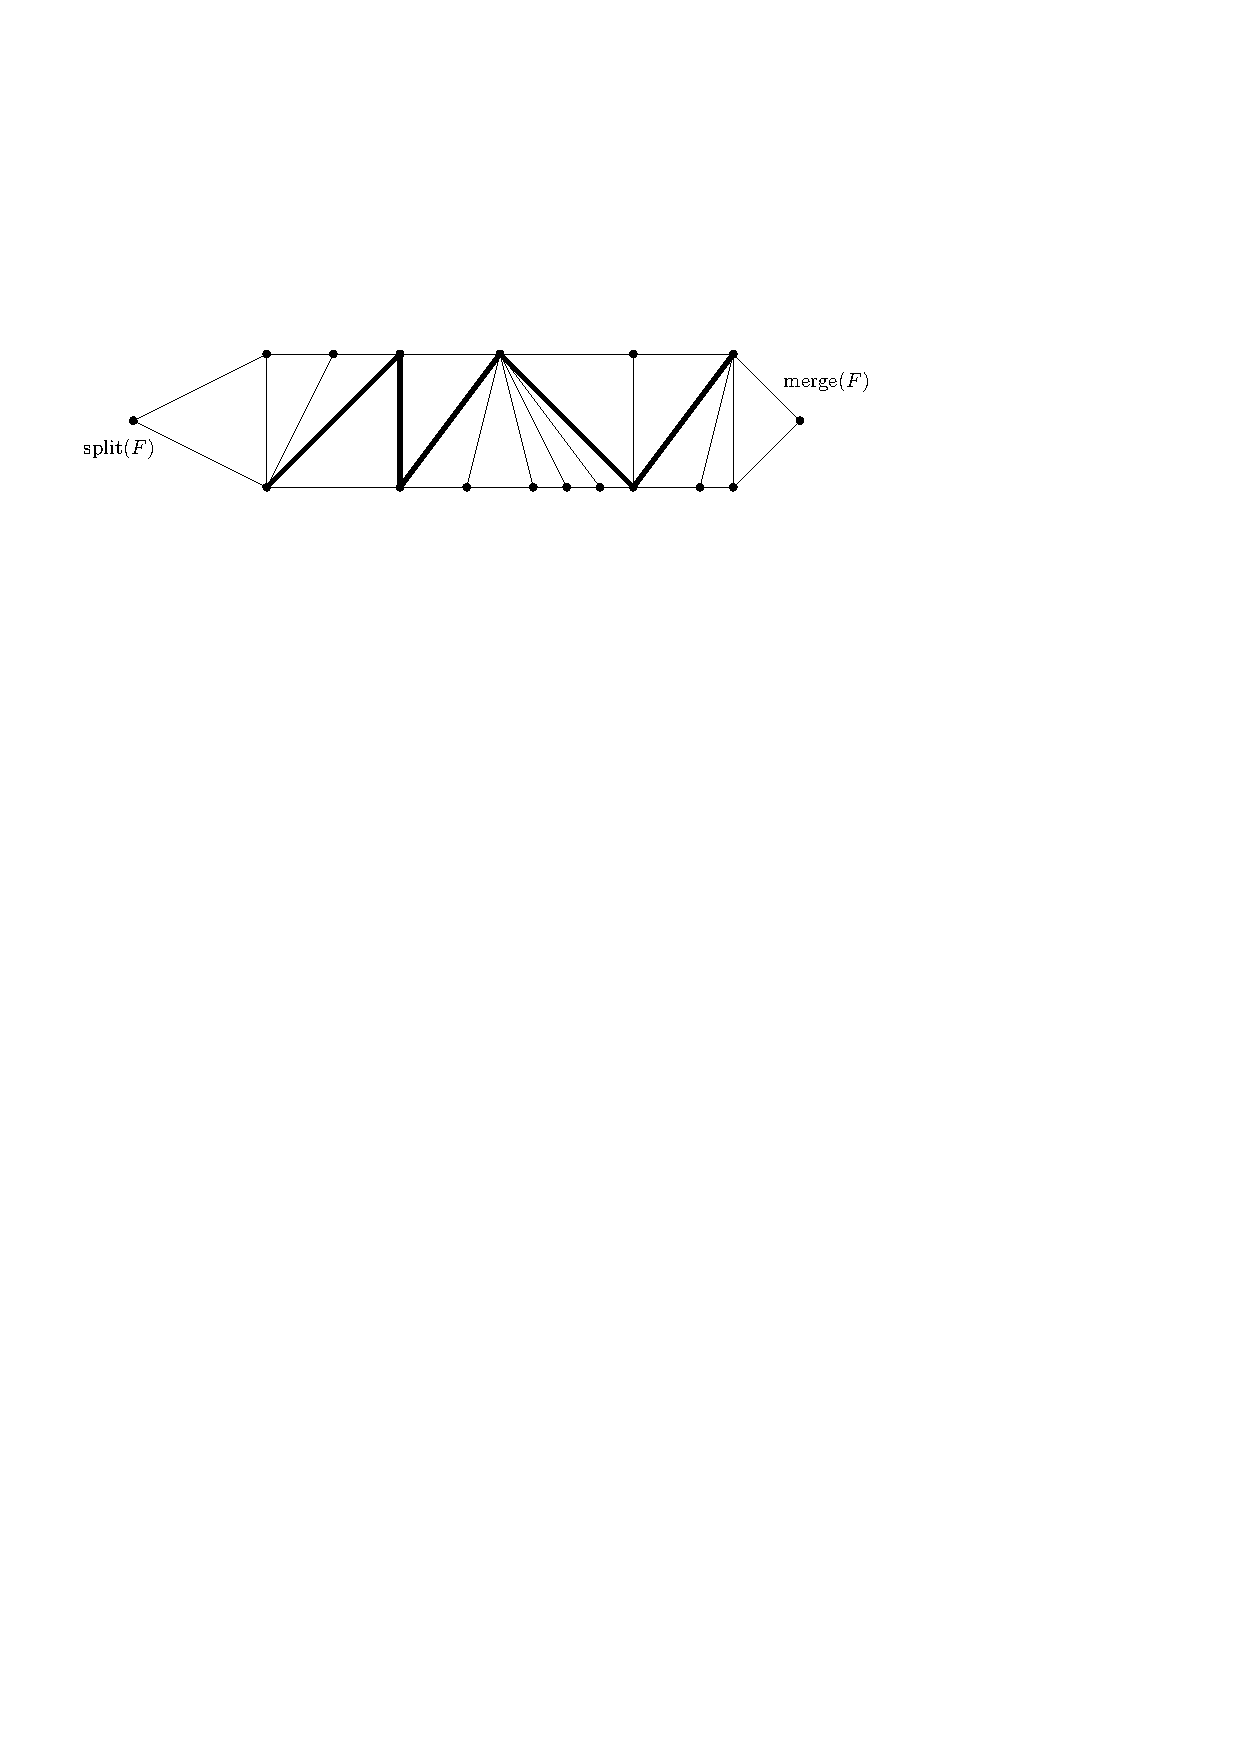
\includegraphics[scale=.9]{rectangularDuals/img/fans}
\clearpage% page: 33
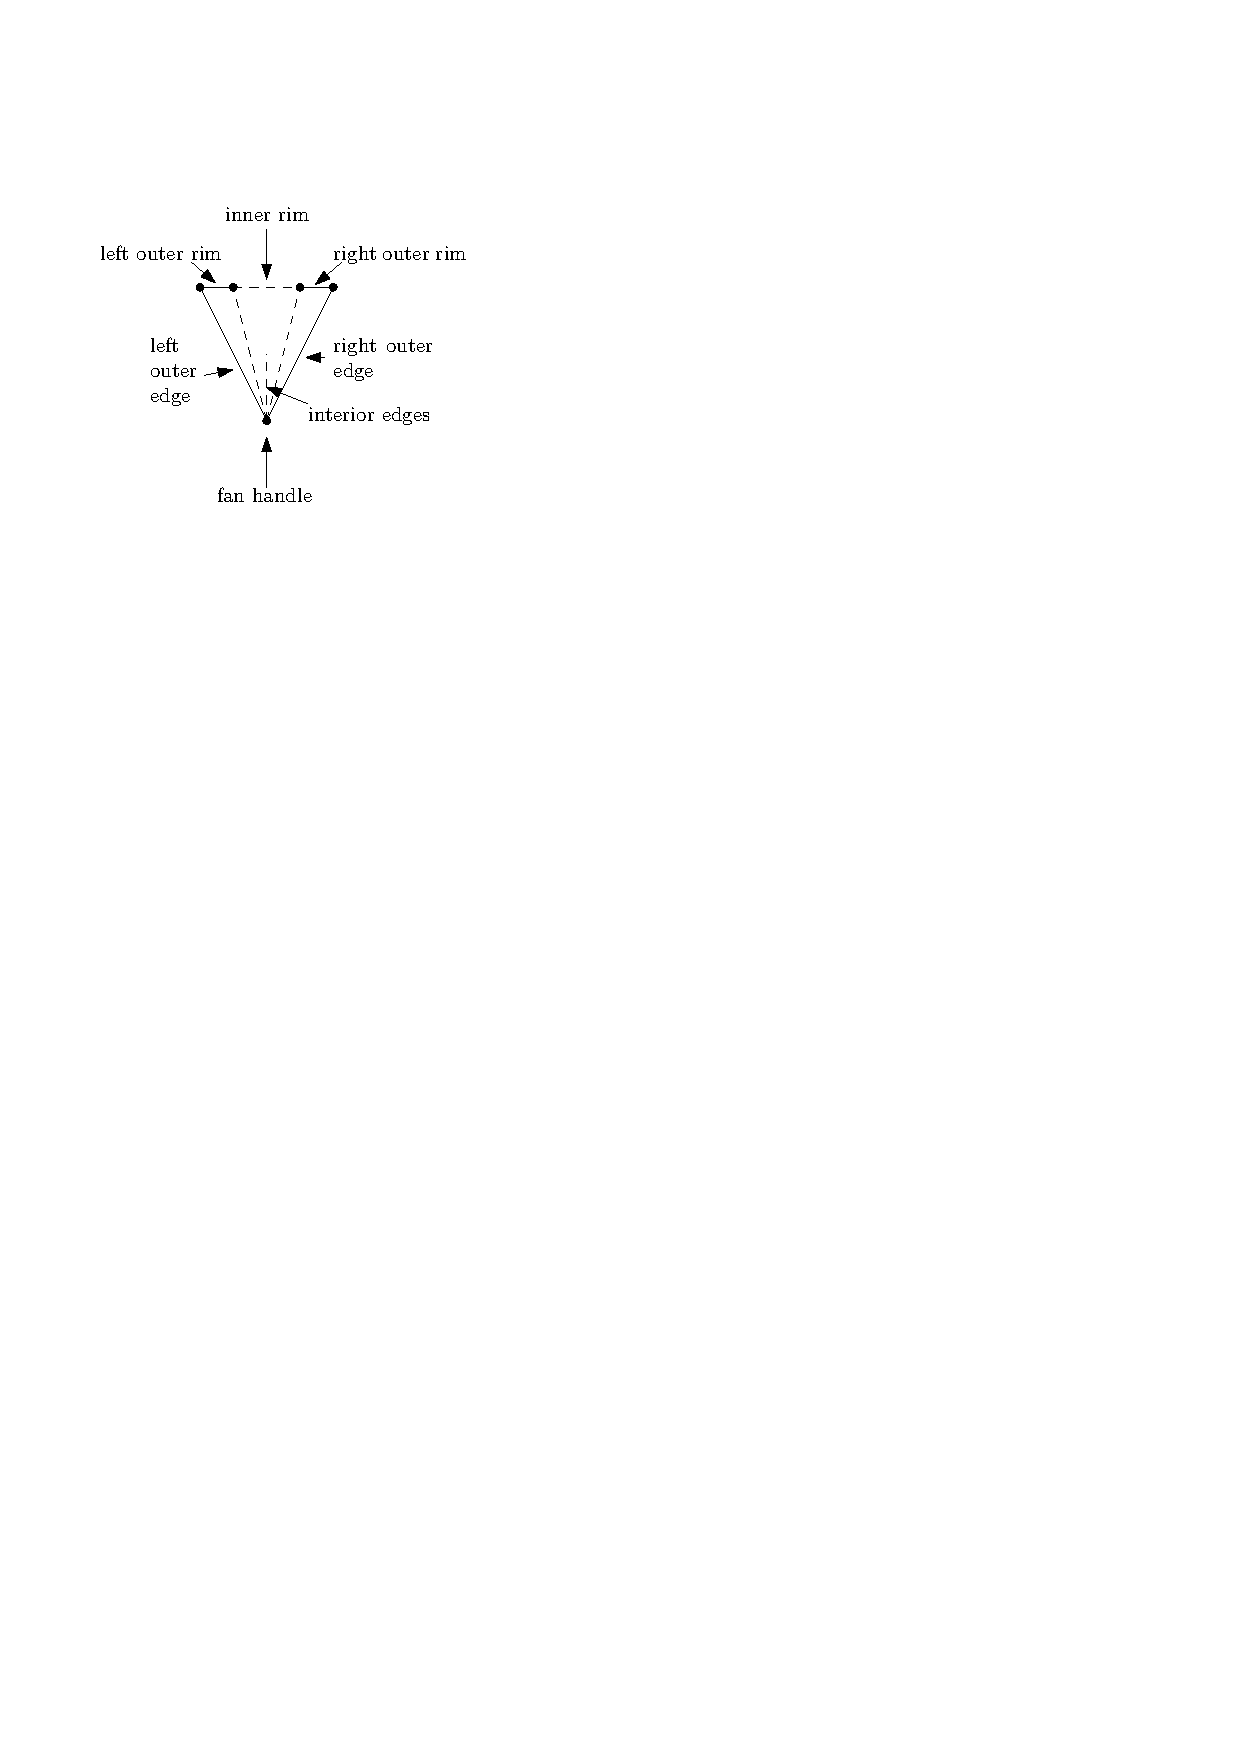
\includegraphics[scale=1]{rectangularDuals/img/fanterms}
\clearpage% page: 34
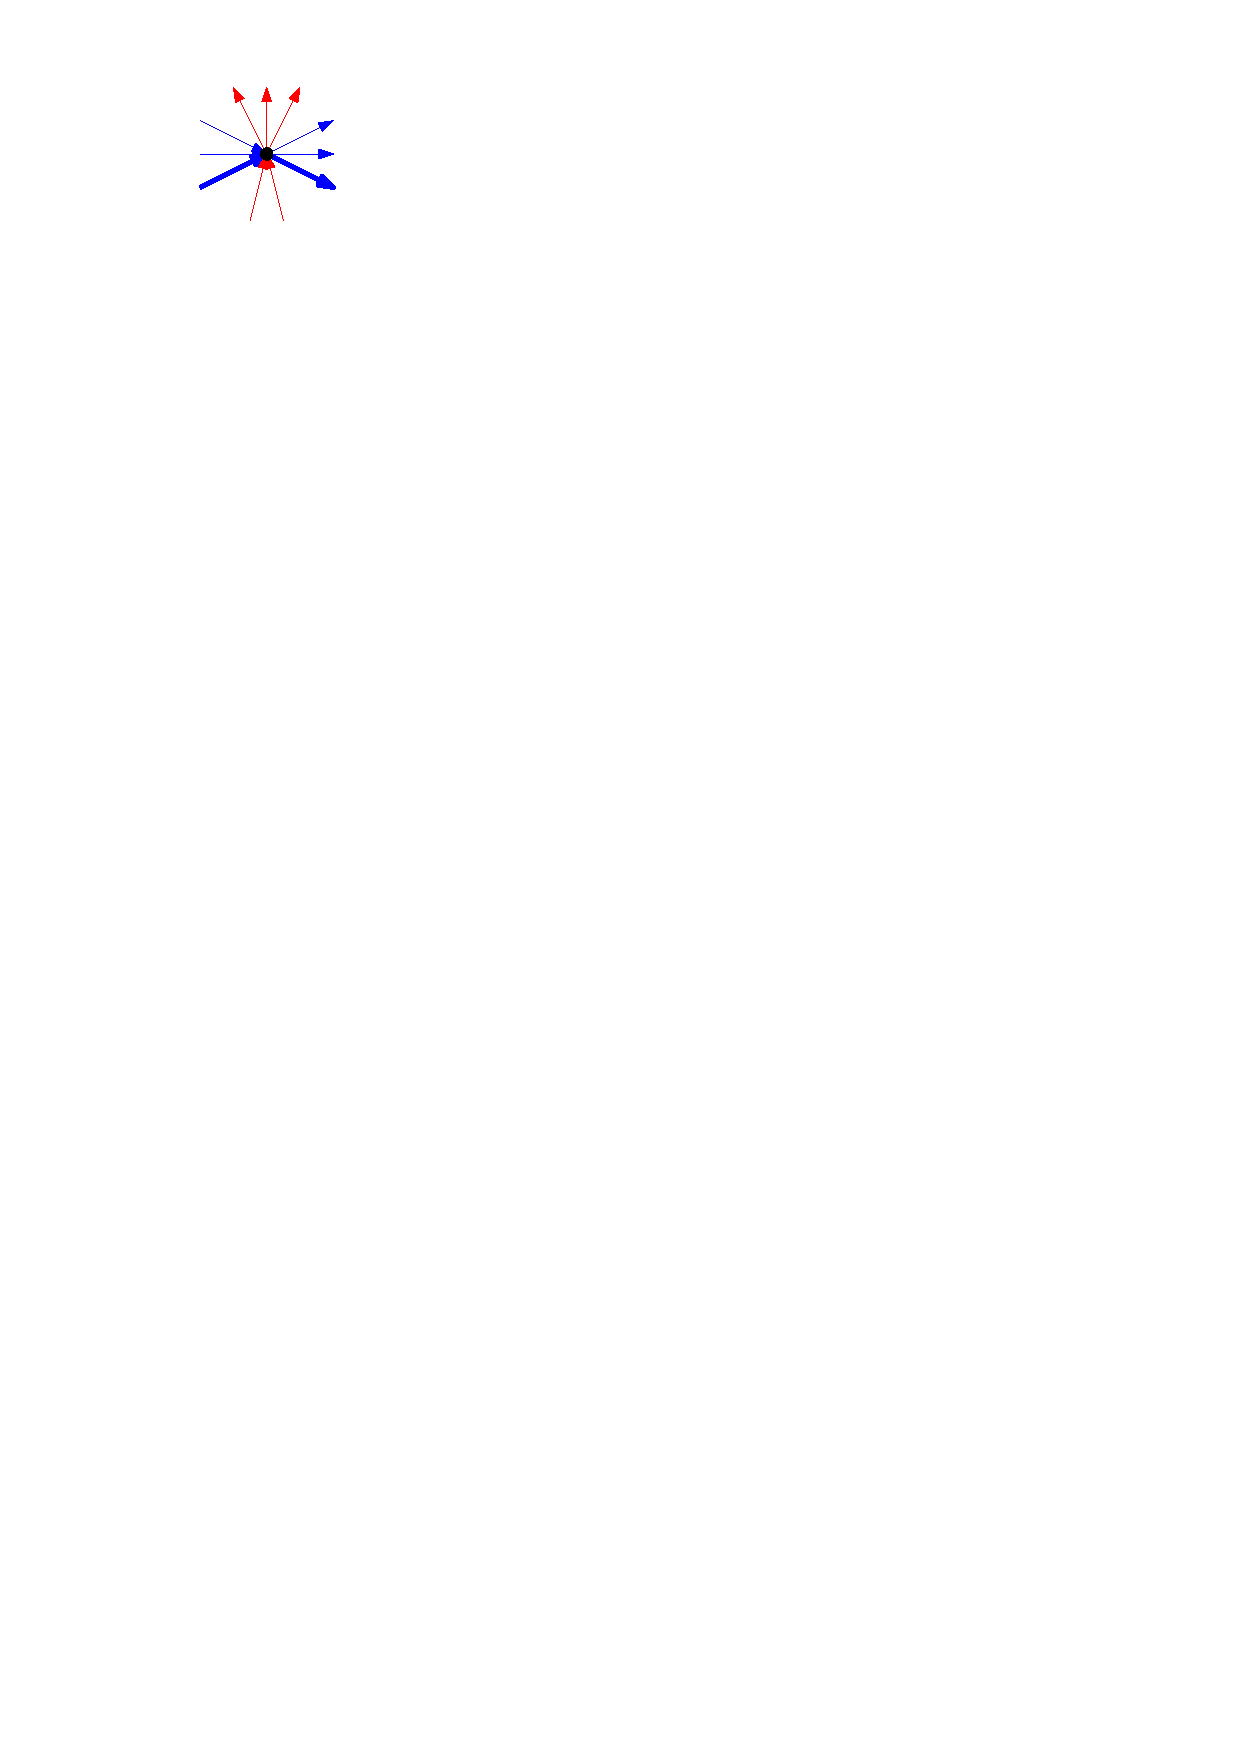
\includegraphics[scale=.9]{./unifiedAlgo/img/sweep/bottompath.pdf}
\clearpage% page: 35
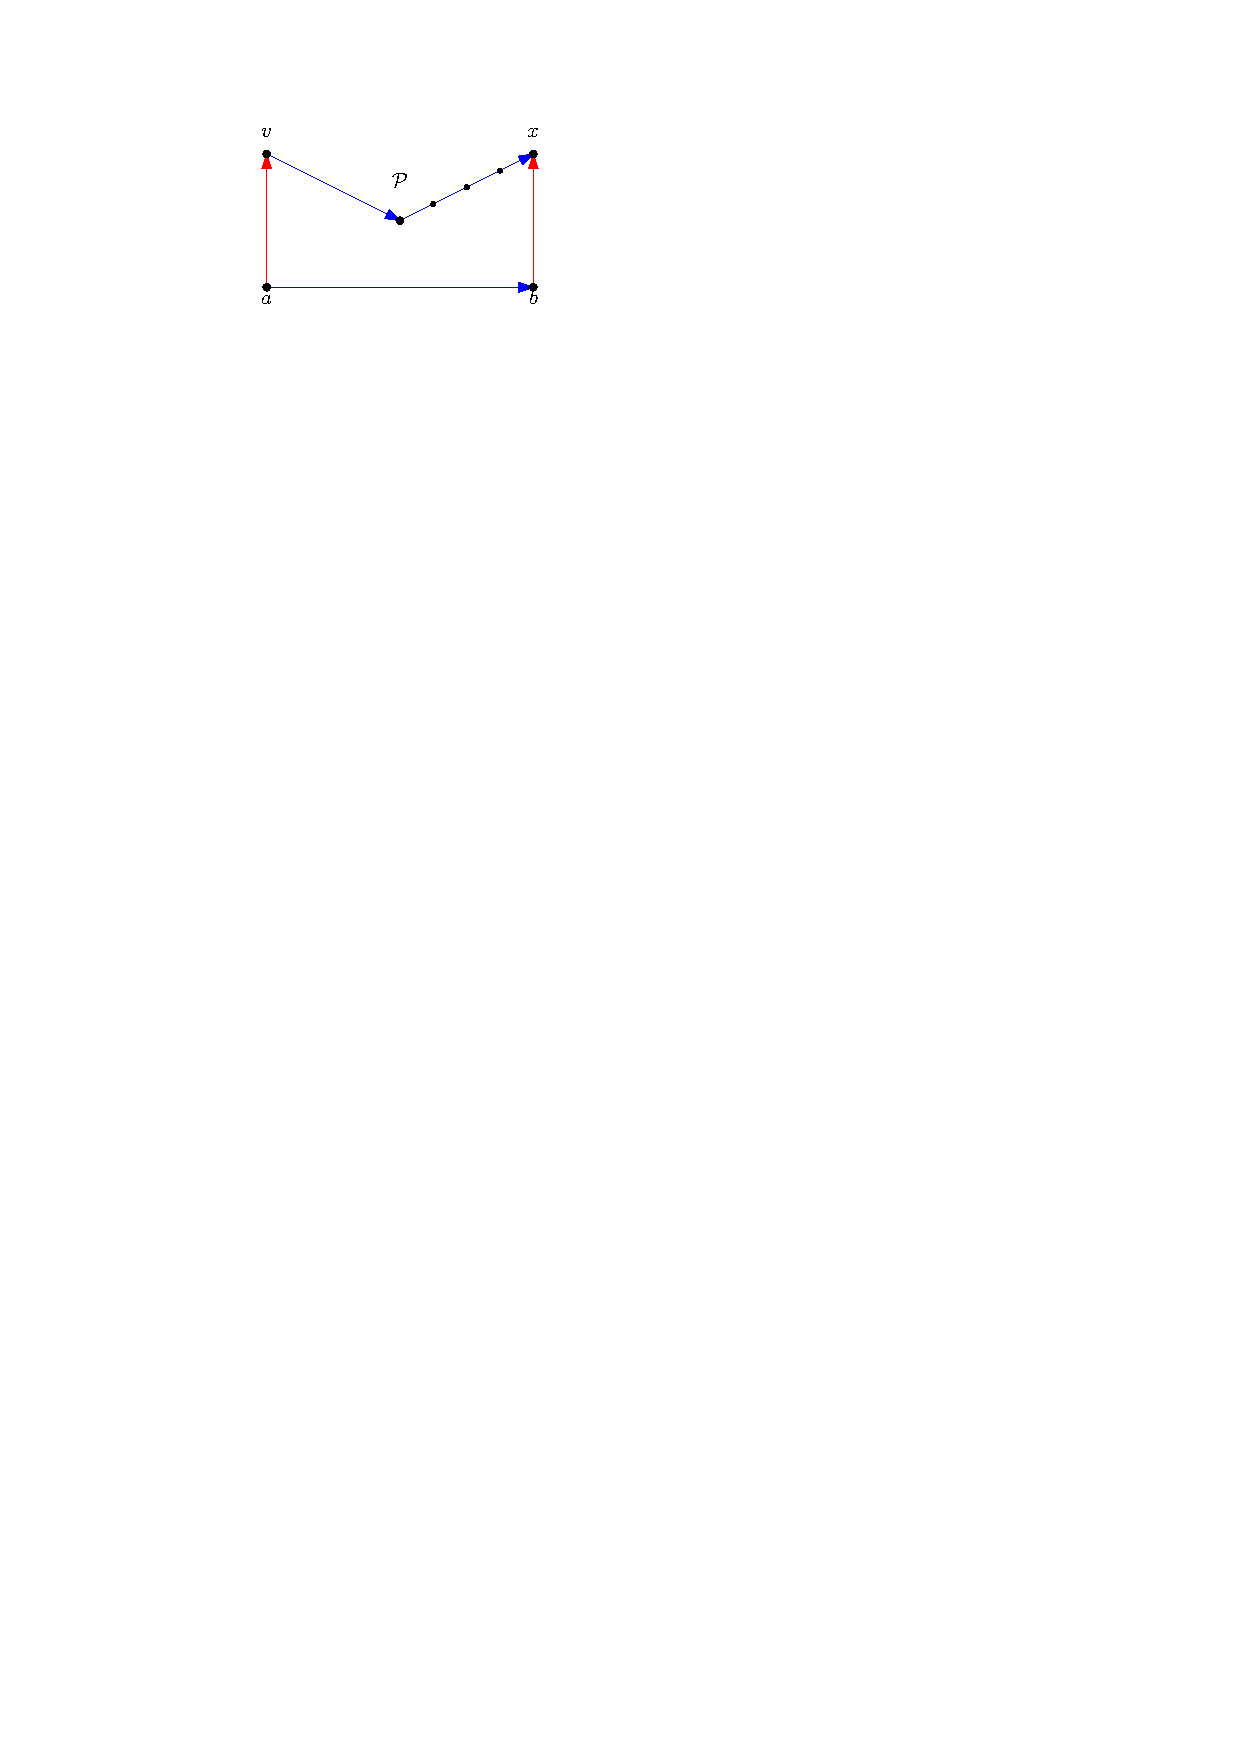
\includegraphics[scale=1]{./unifiedAlgo/img/sweep/bottompathChord.pdf}
\clearpage% page: 36
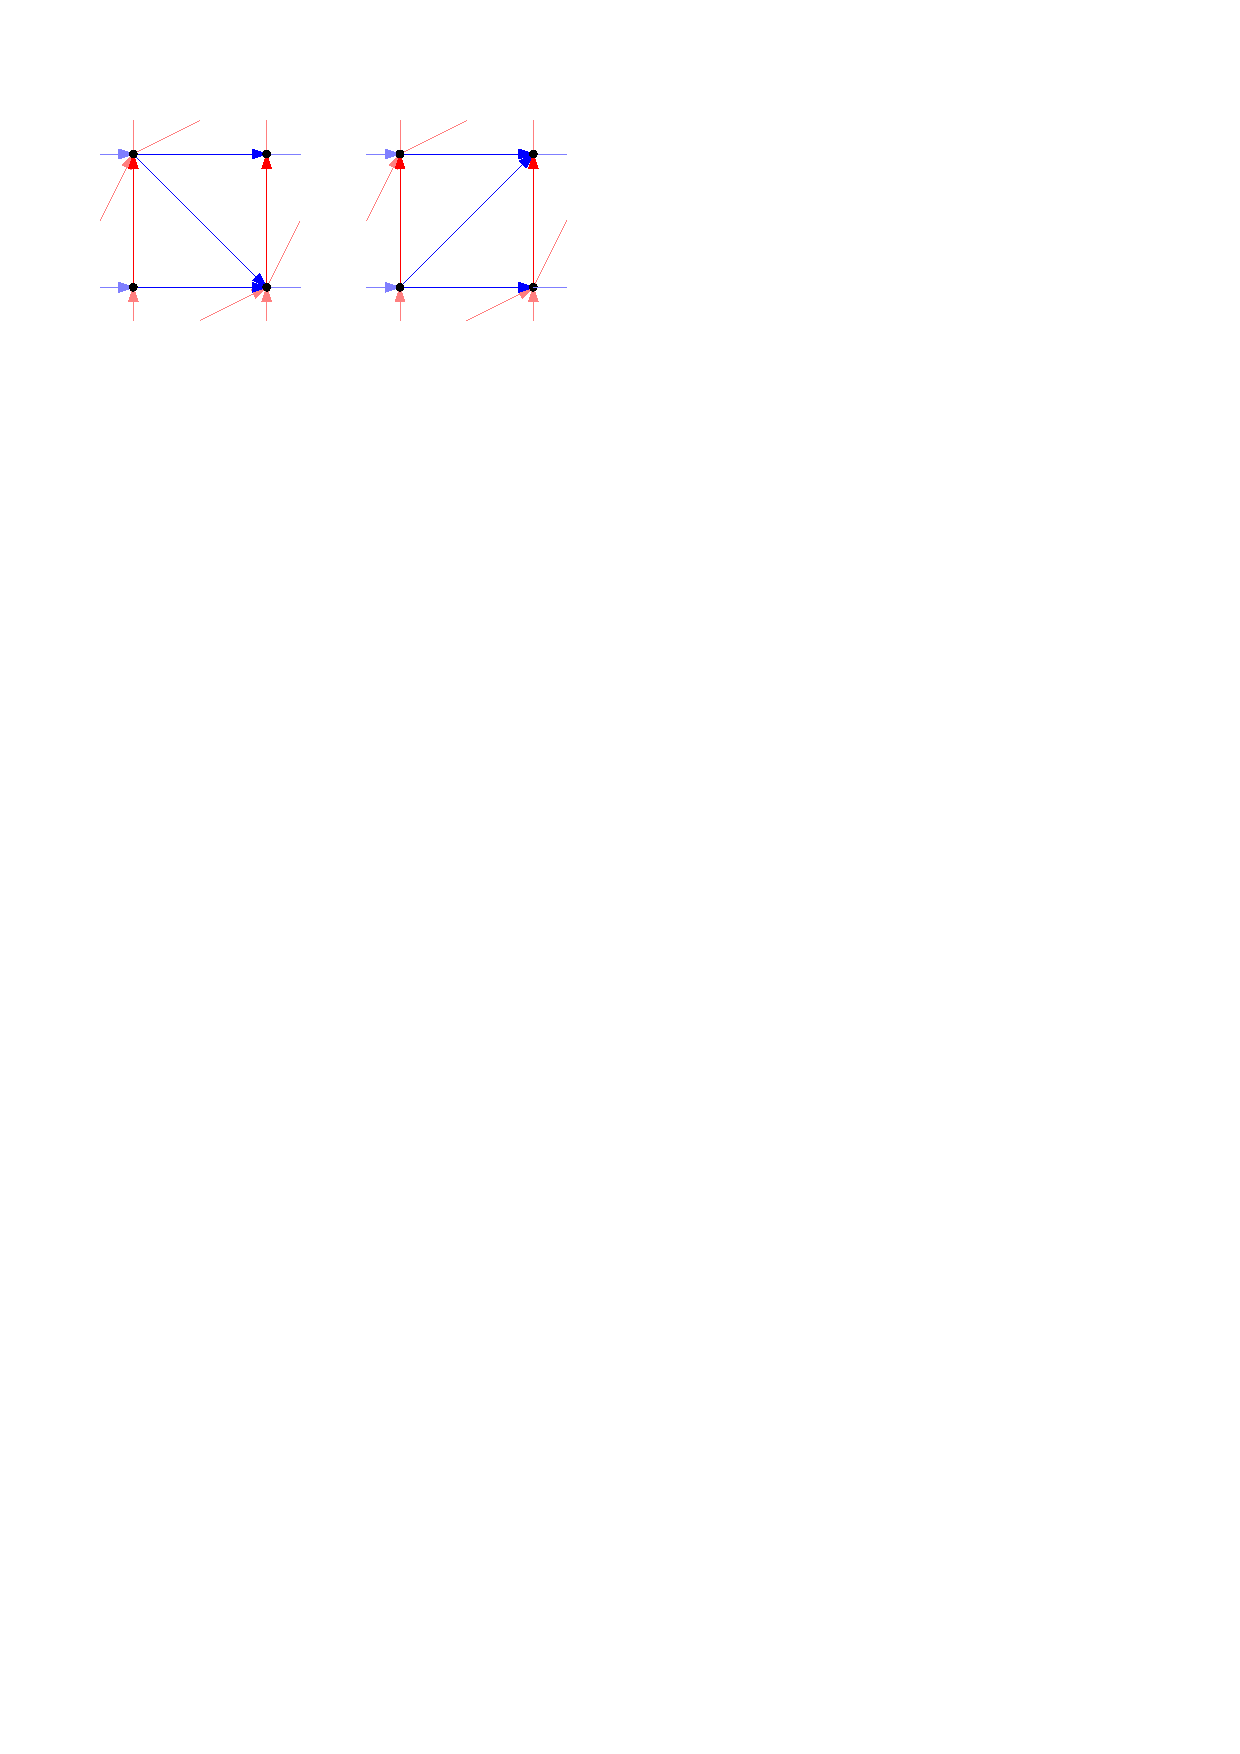
\includegraphics[scale=1]{./unifiedAlgo/img/zflip/blueZ.pdf}
\clearpage% page: 37
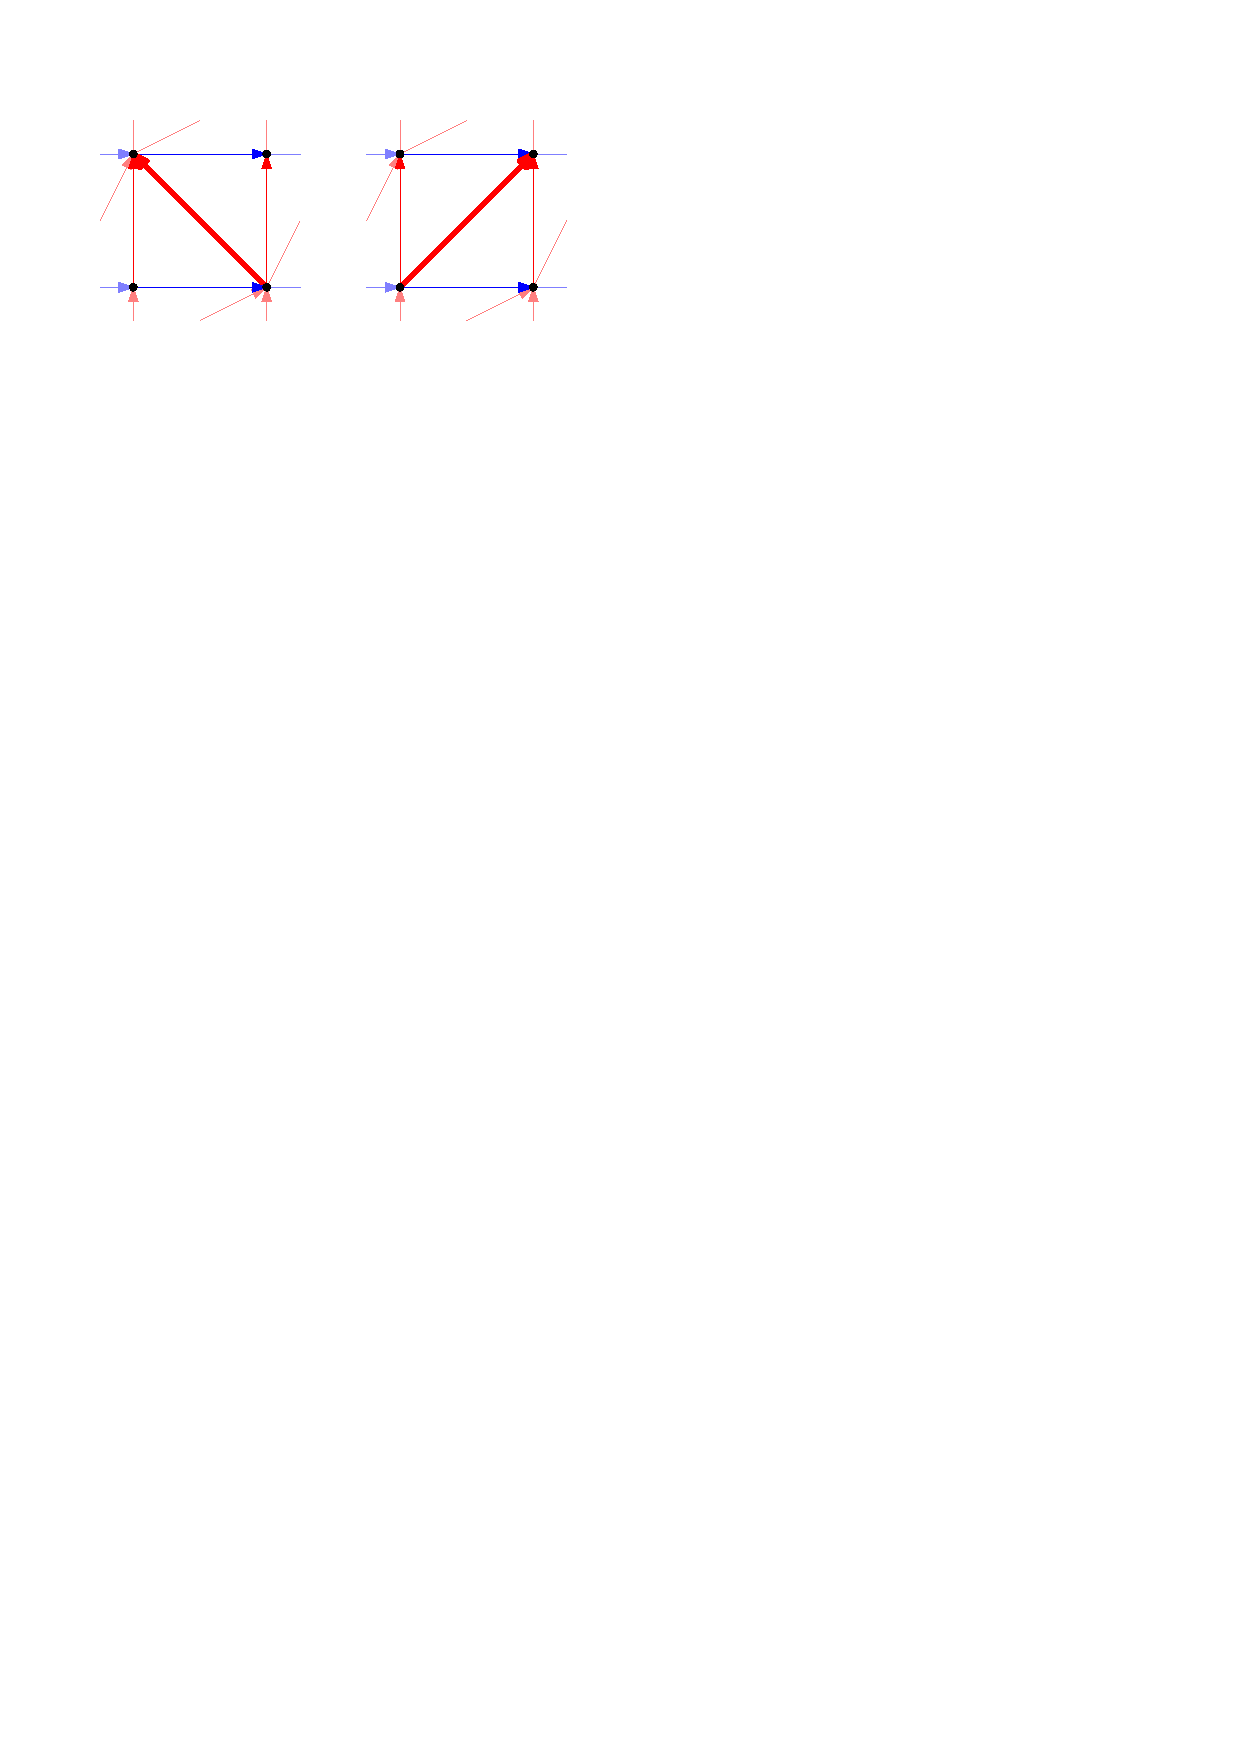
\includegraphics[scale=1]{./unifiedAlgo/img/zflip/flip.pdf}
\clearpage% page: 38
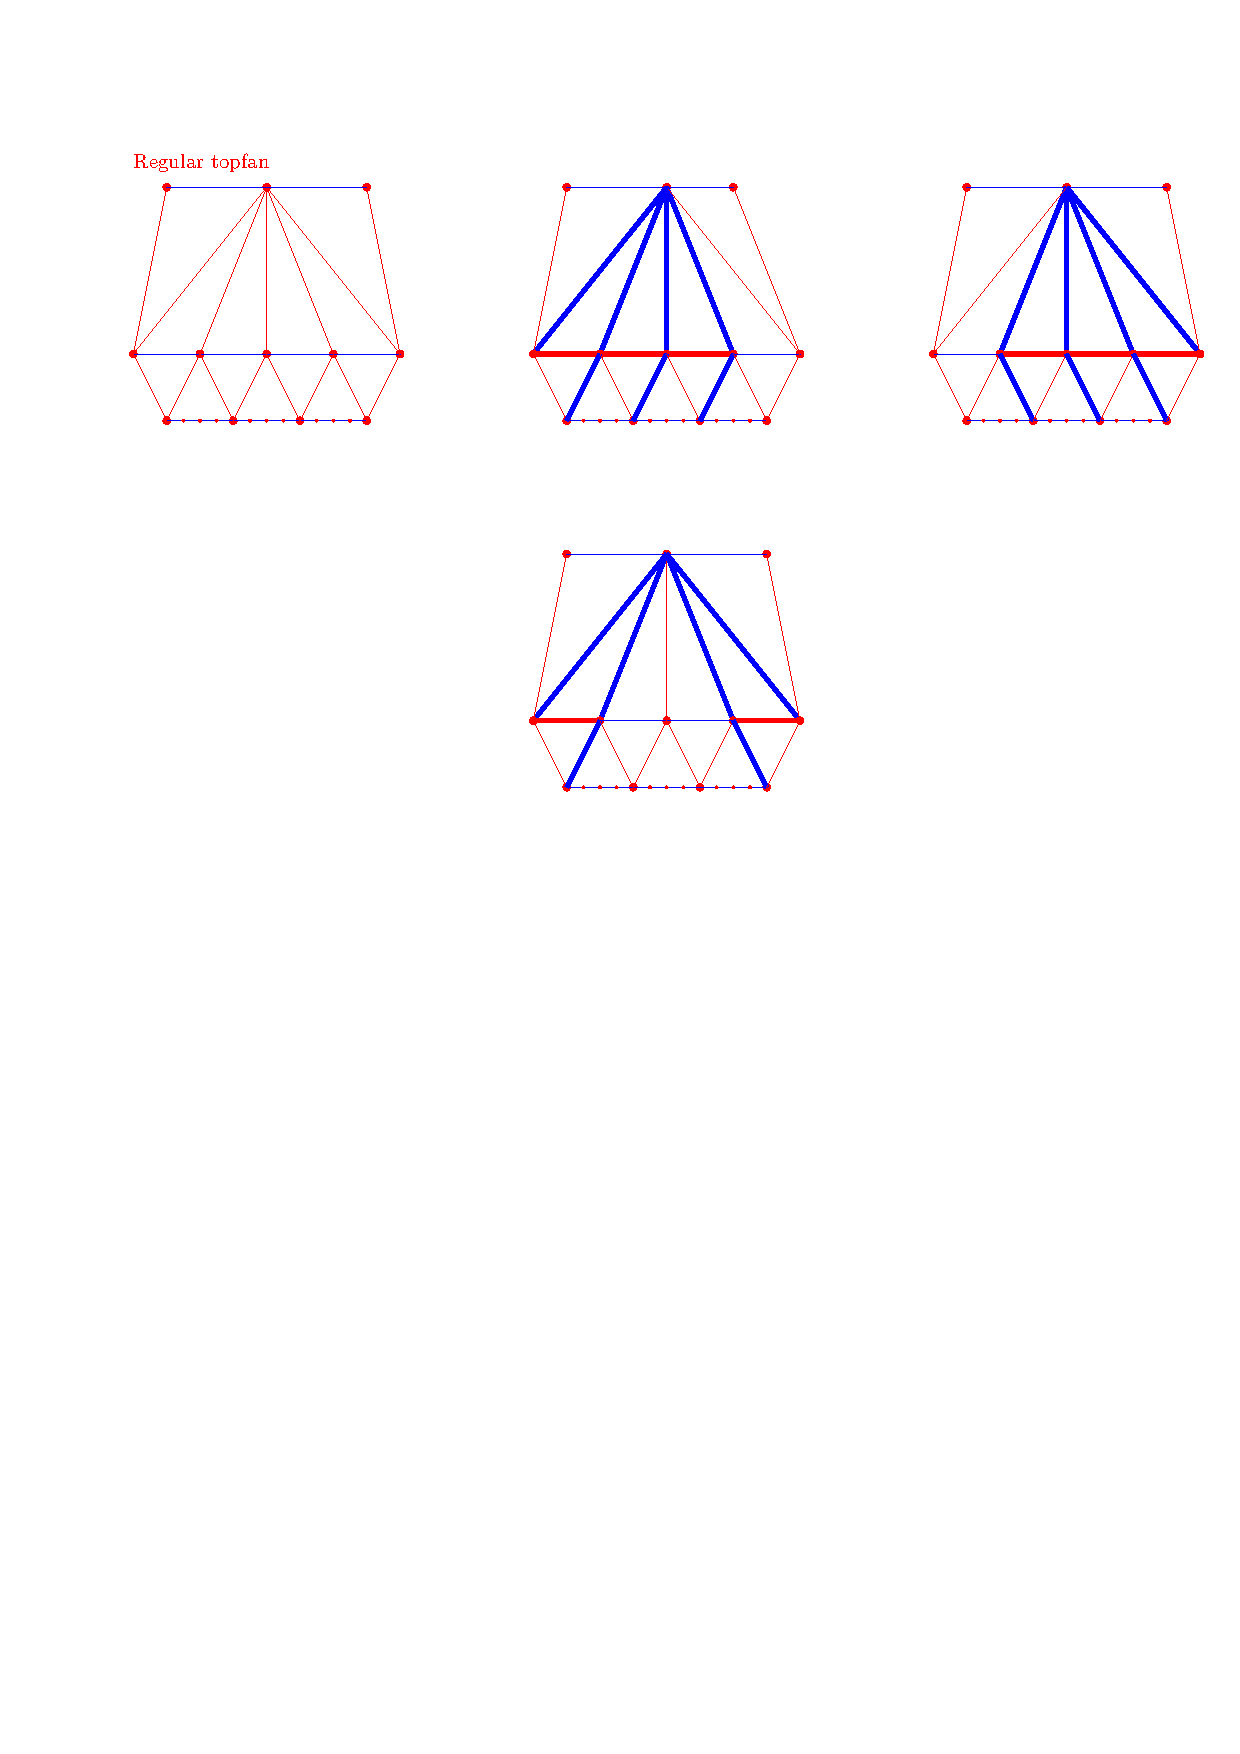
\includegraphics[width = \textwidth]{topFanFlips/img/regular}
\clearpage% page: 39
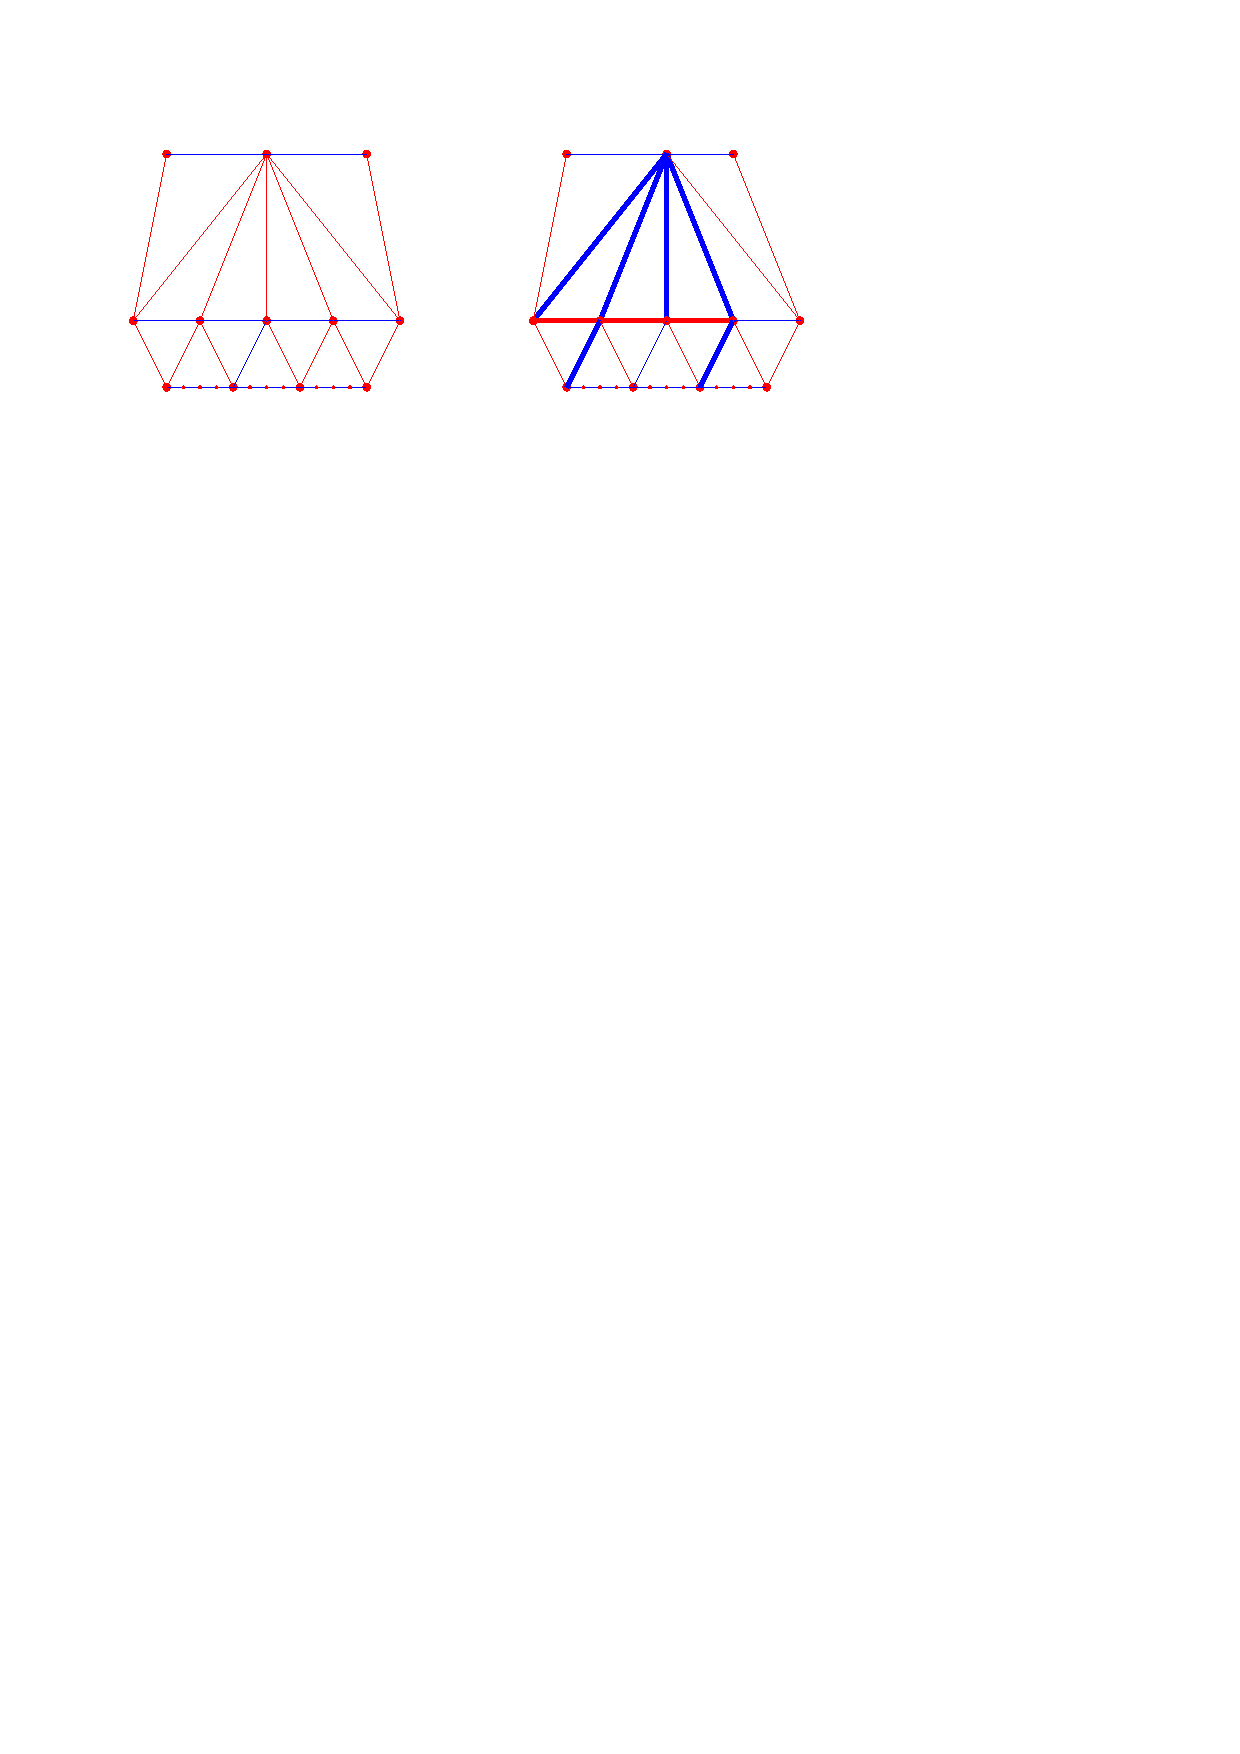
\includegraphics[width = \textwidth]{topFanFlips/img/merge}
\clearpage% page: 40
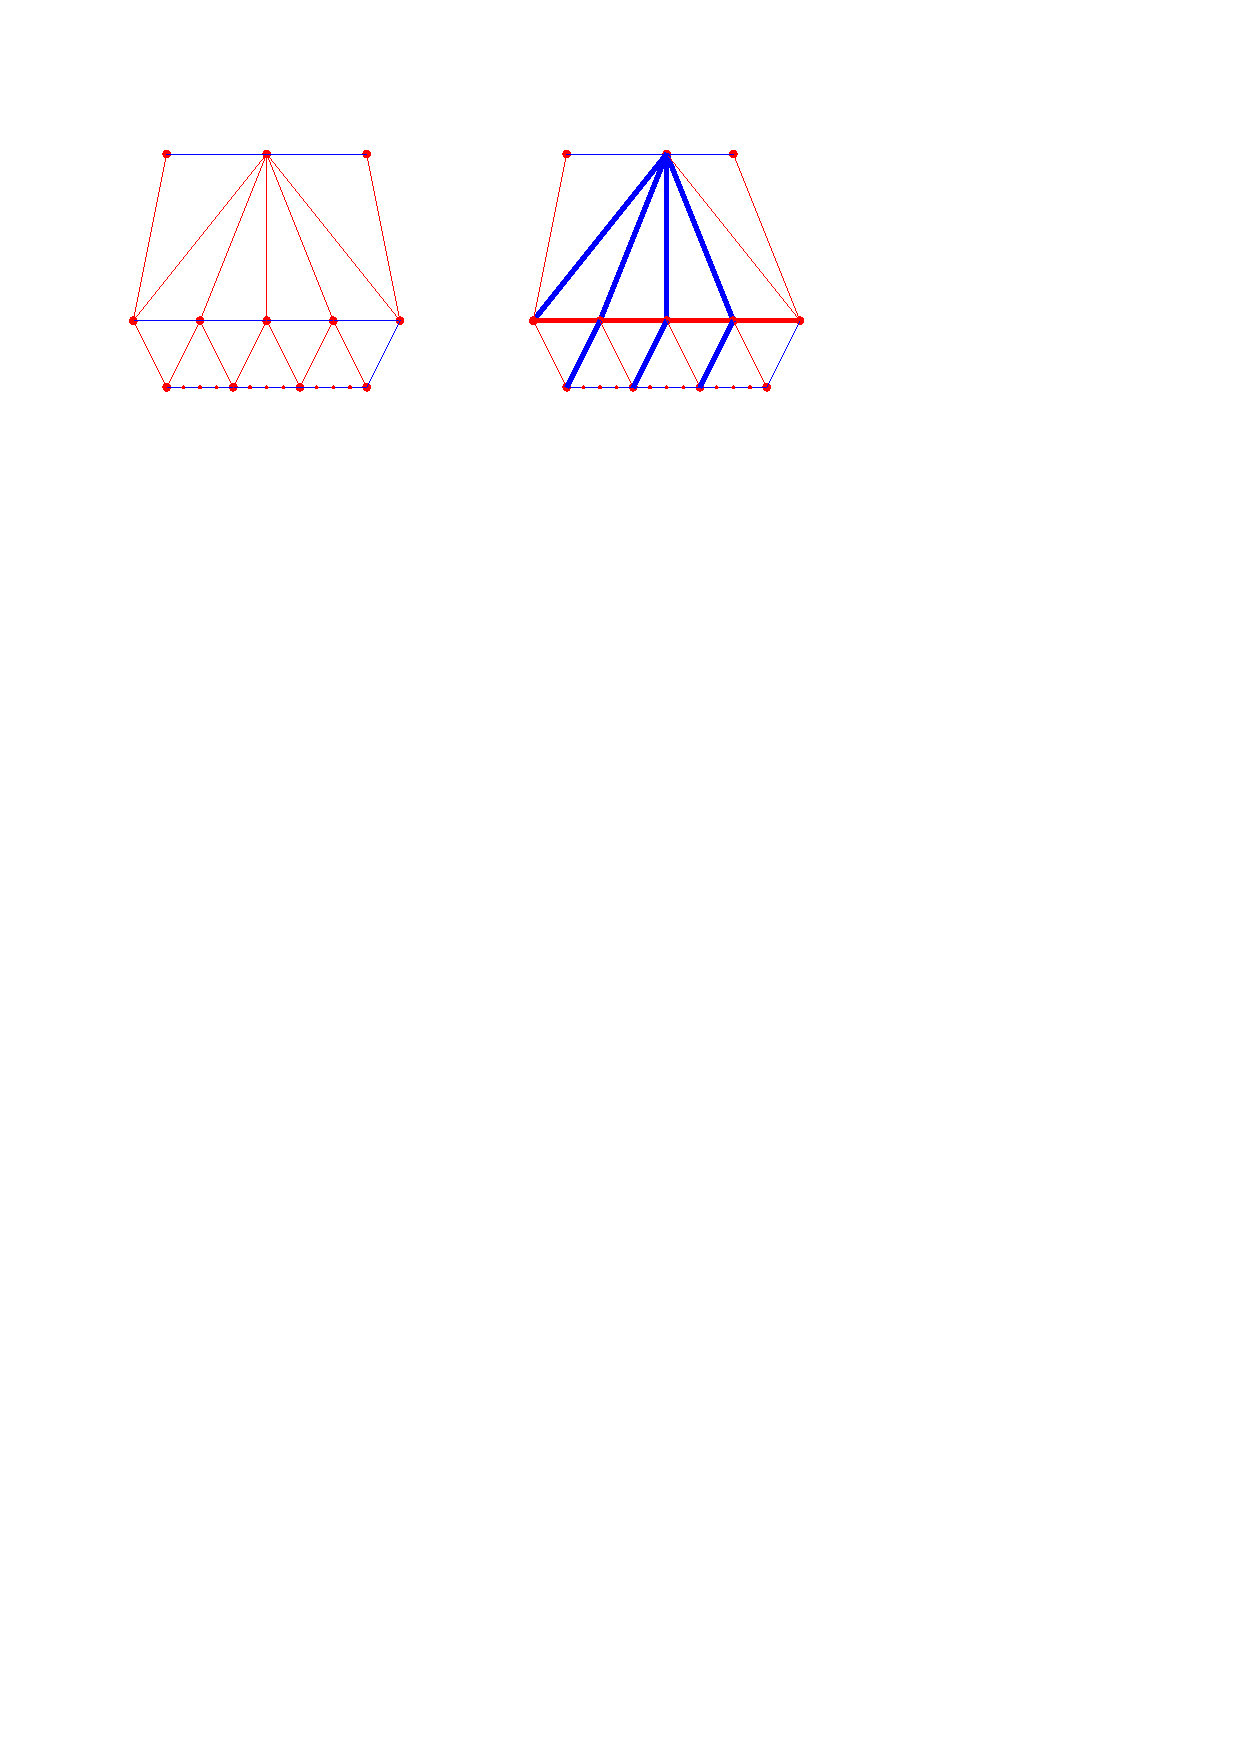
\includegraphics[width =\textwidth]{topFanFlips/img/mergeend}
\clearpage% page: 41
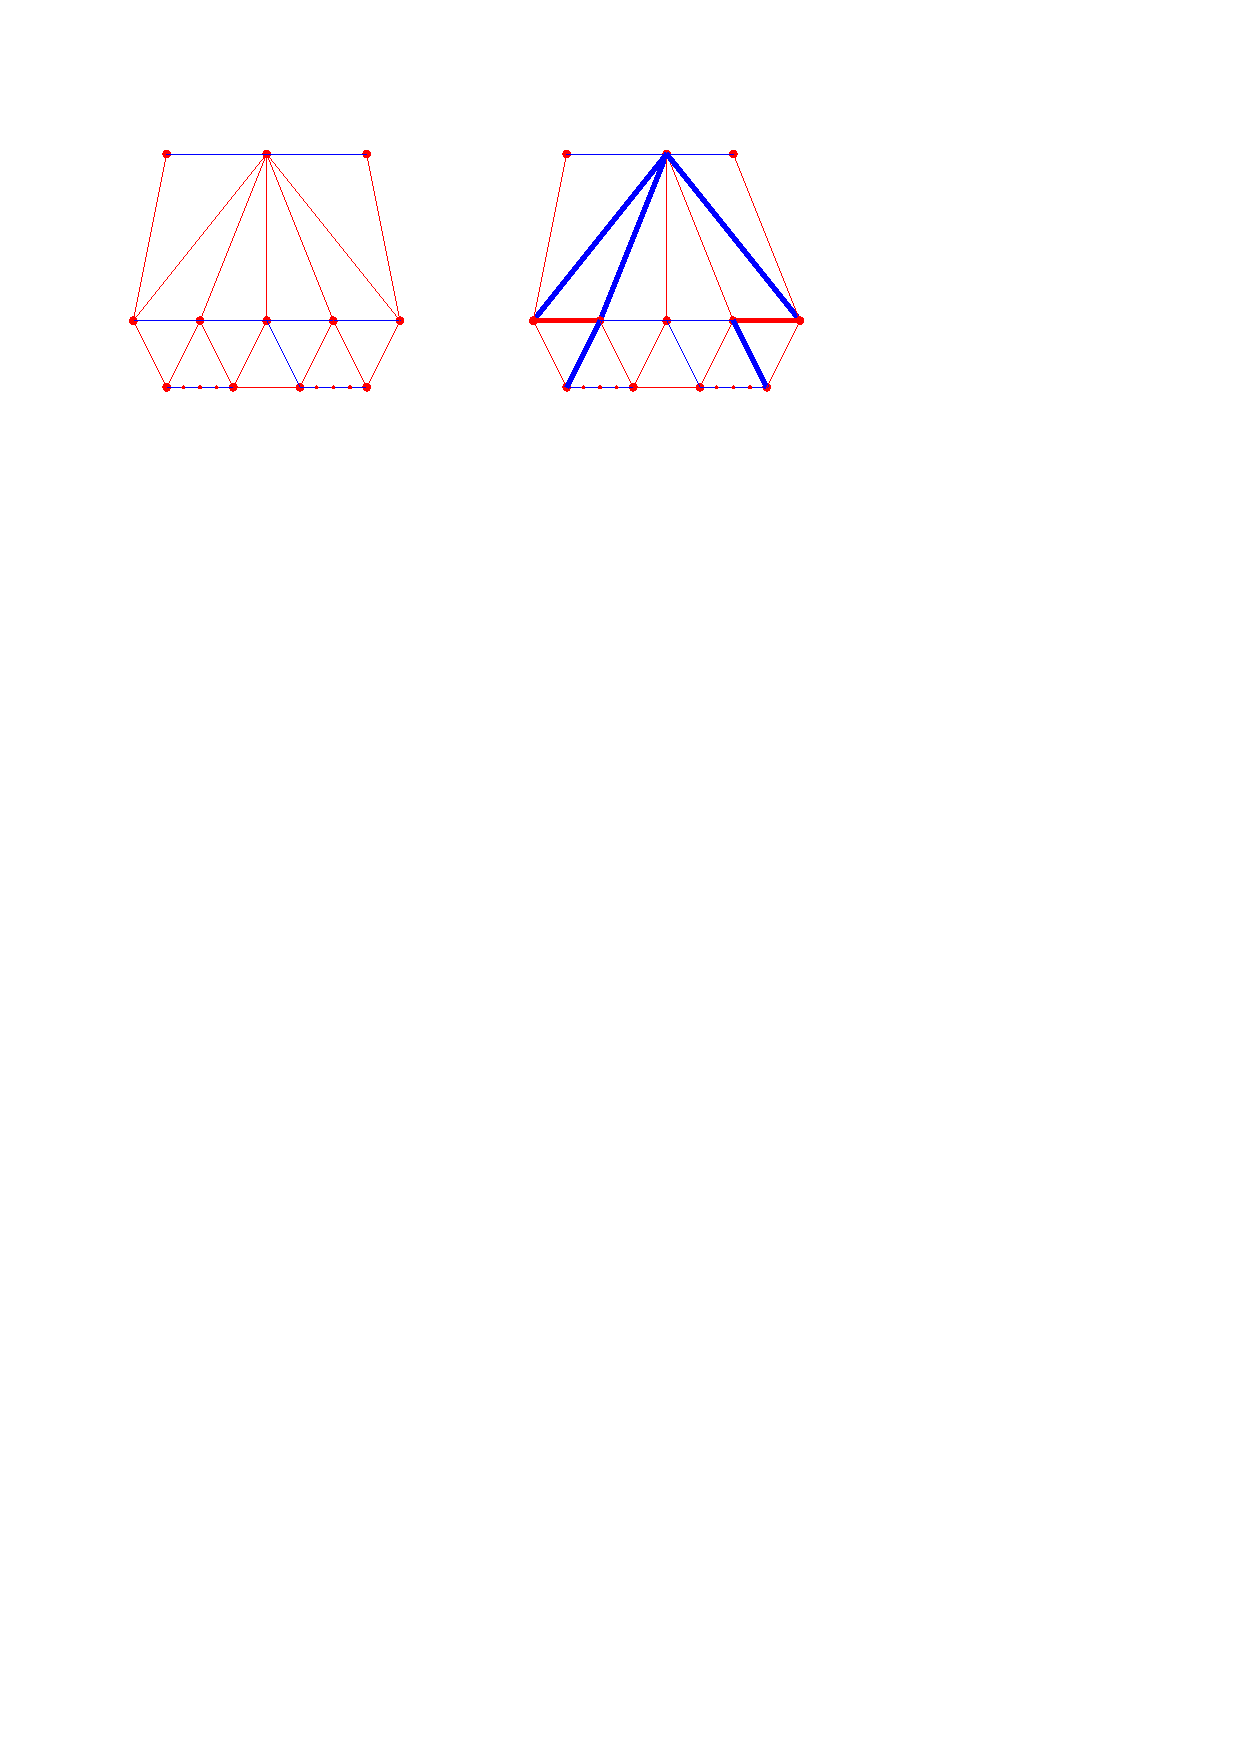
\includegraphics[width = \textwidth]{topFanFlips/img/split}
\clearpage% page: 42
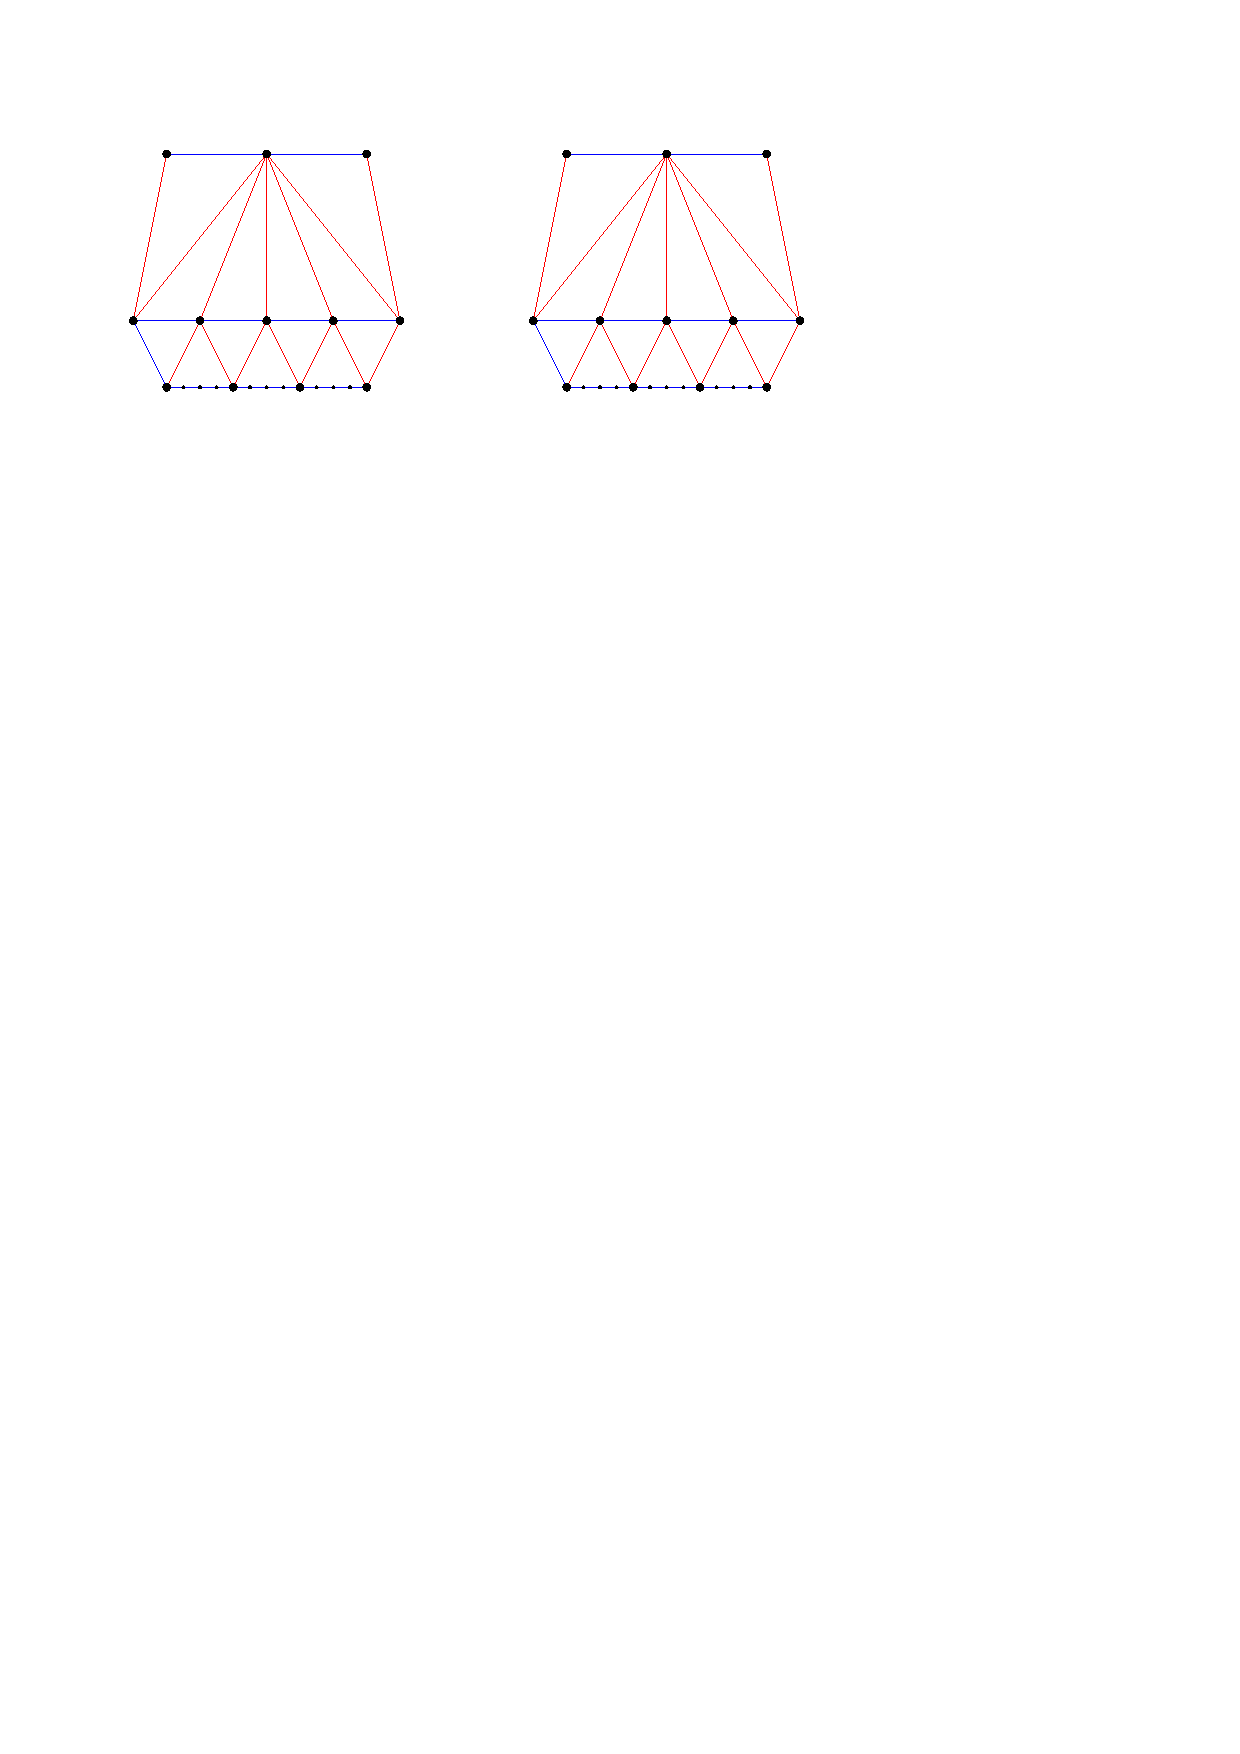
\includegraphics[width =\textwidth]{topFanFlips/img/splitfront}
\clearpage% page: 43
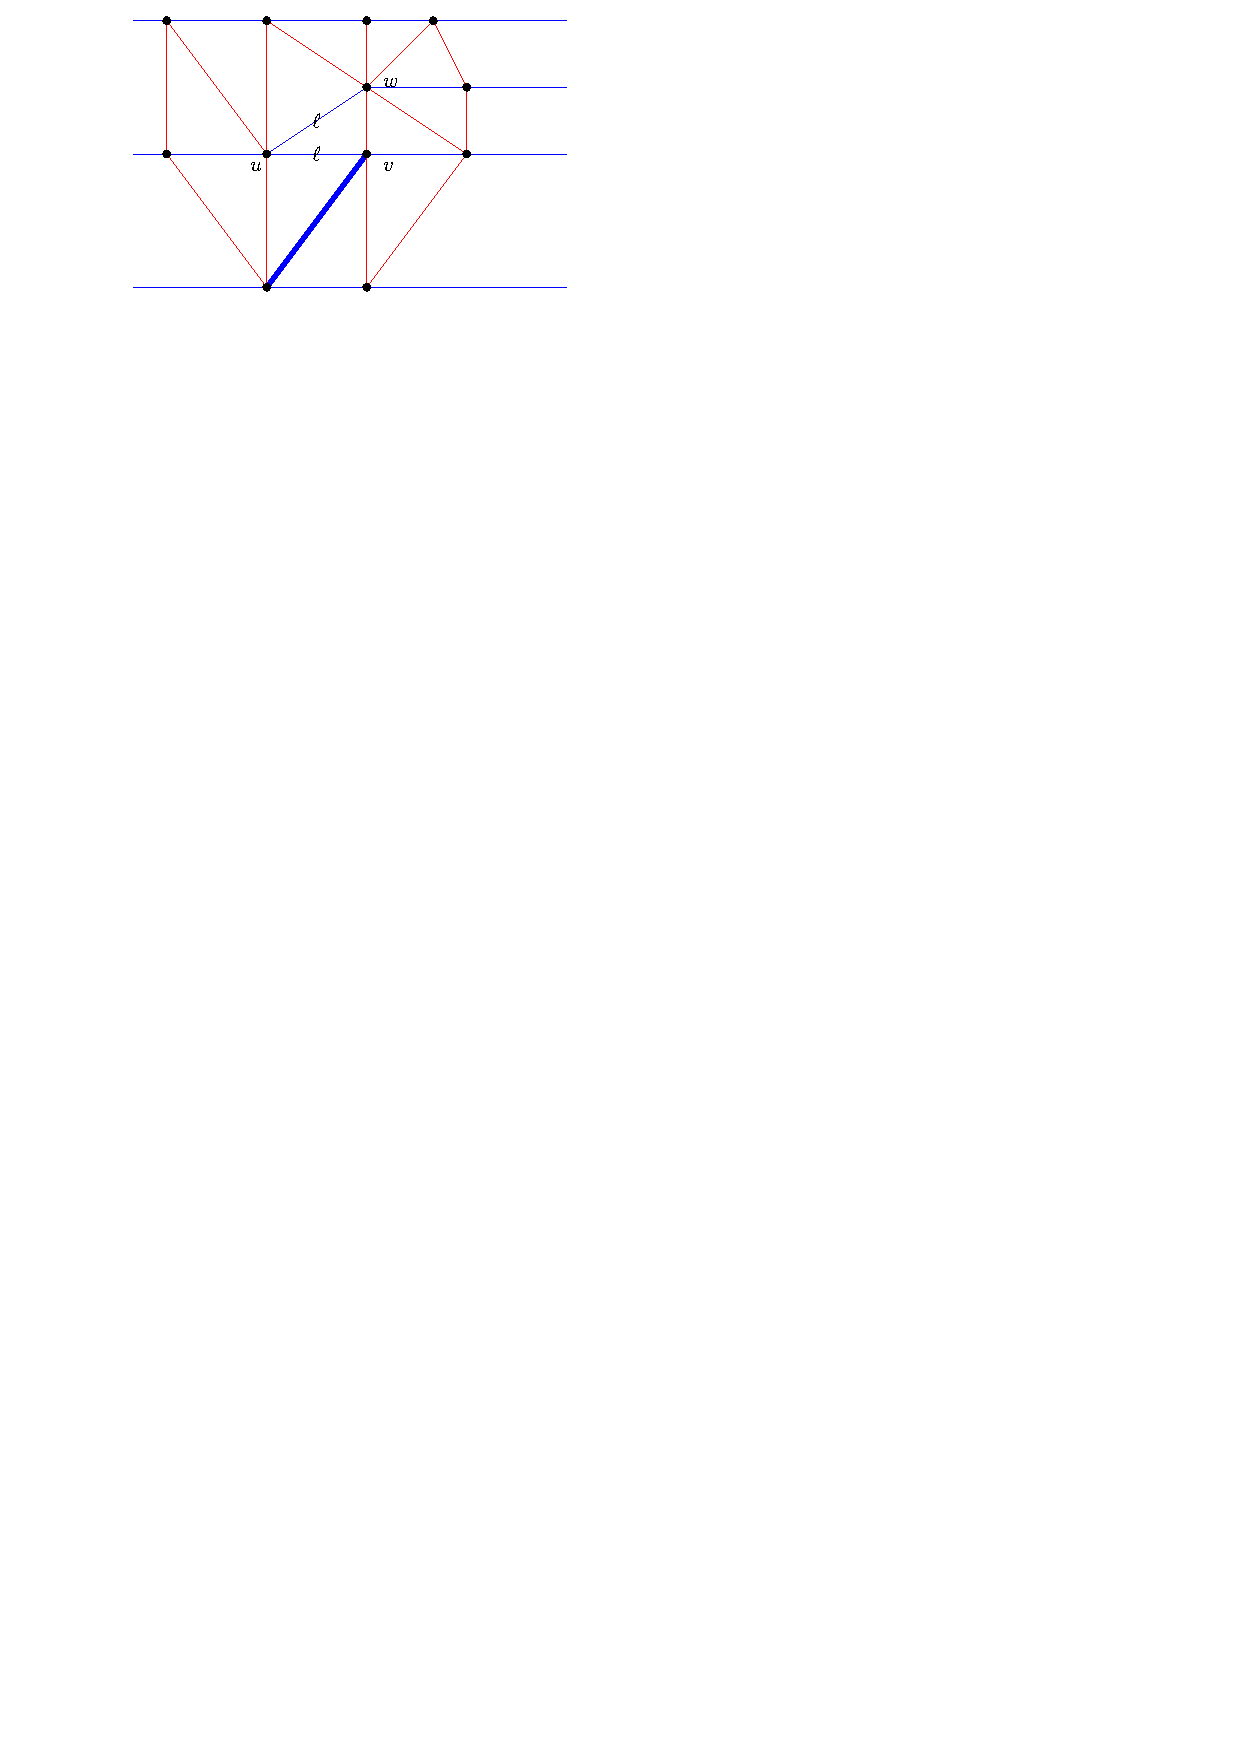
\includegraphics[scale=1]{./blueFaceSubdivision/img/puttingTroughLoad.pdf}
\clearpage% page: 44
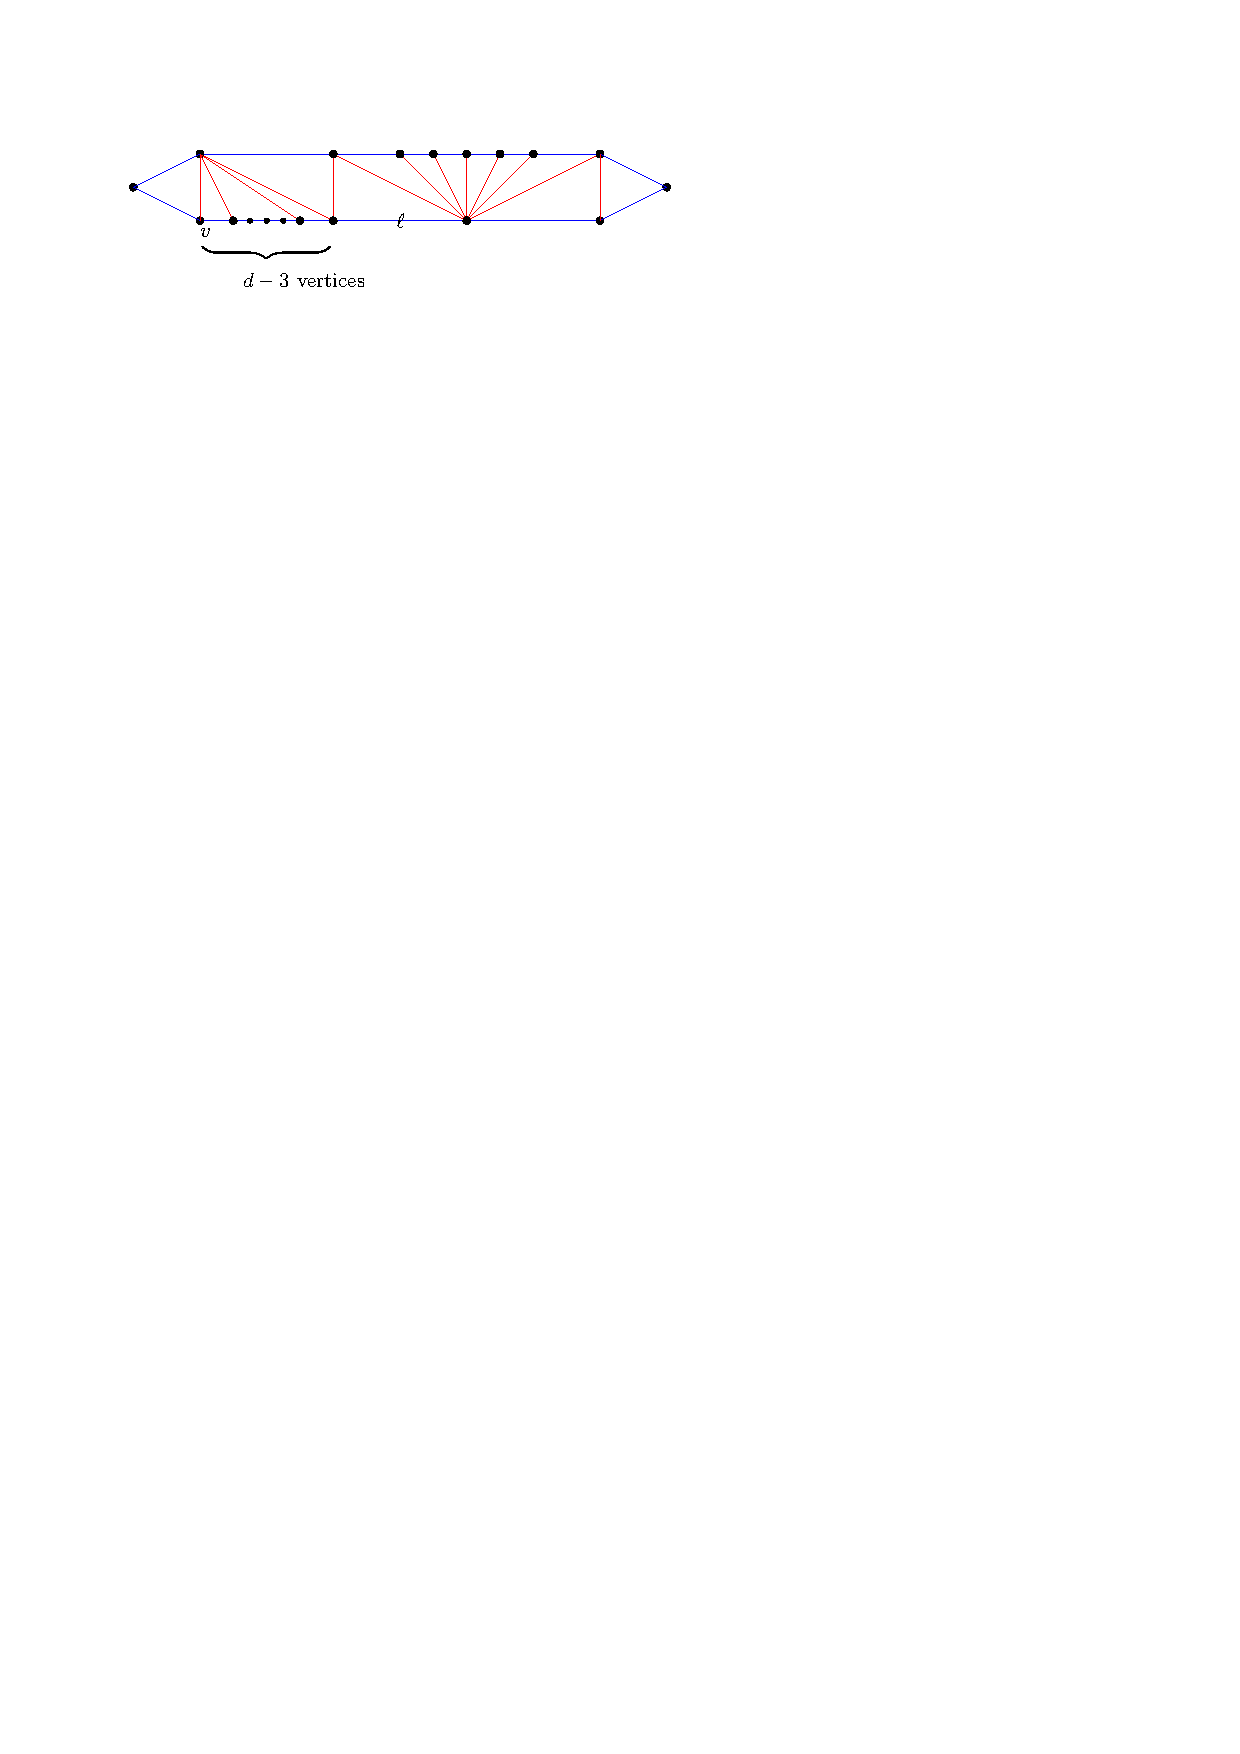
\includegraphics[scale=1]{blueFaceSubdivision/img/worstCaseWithTopFan}
\clearpage% page: 45
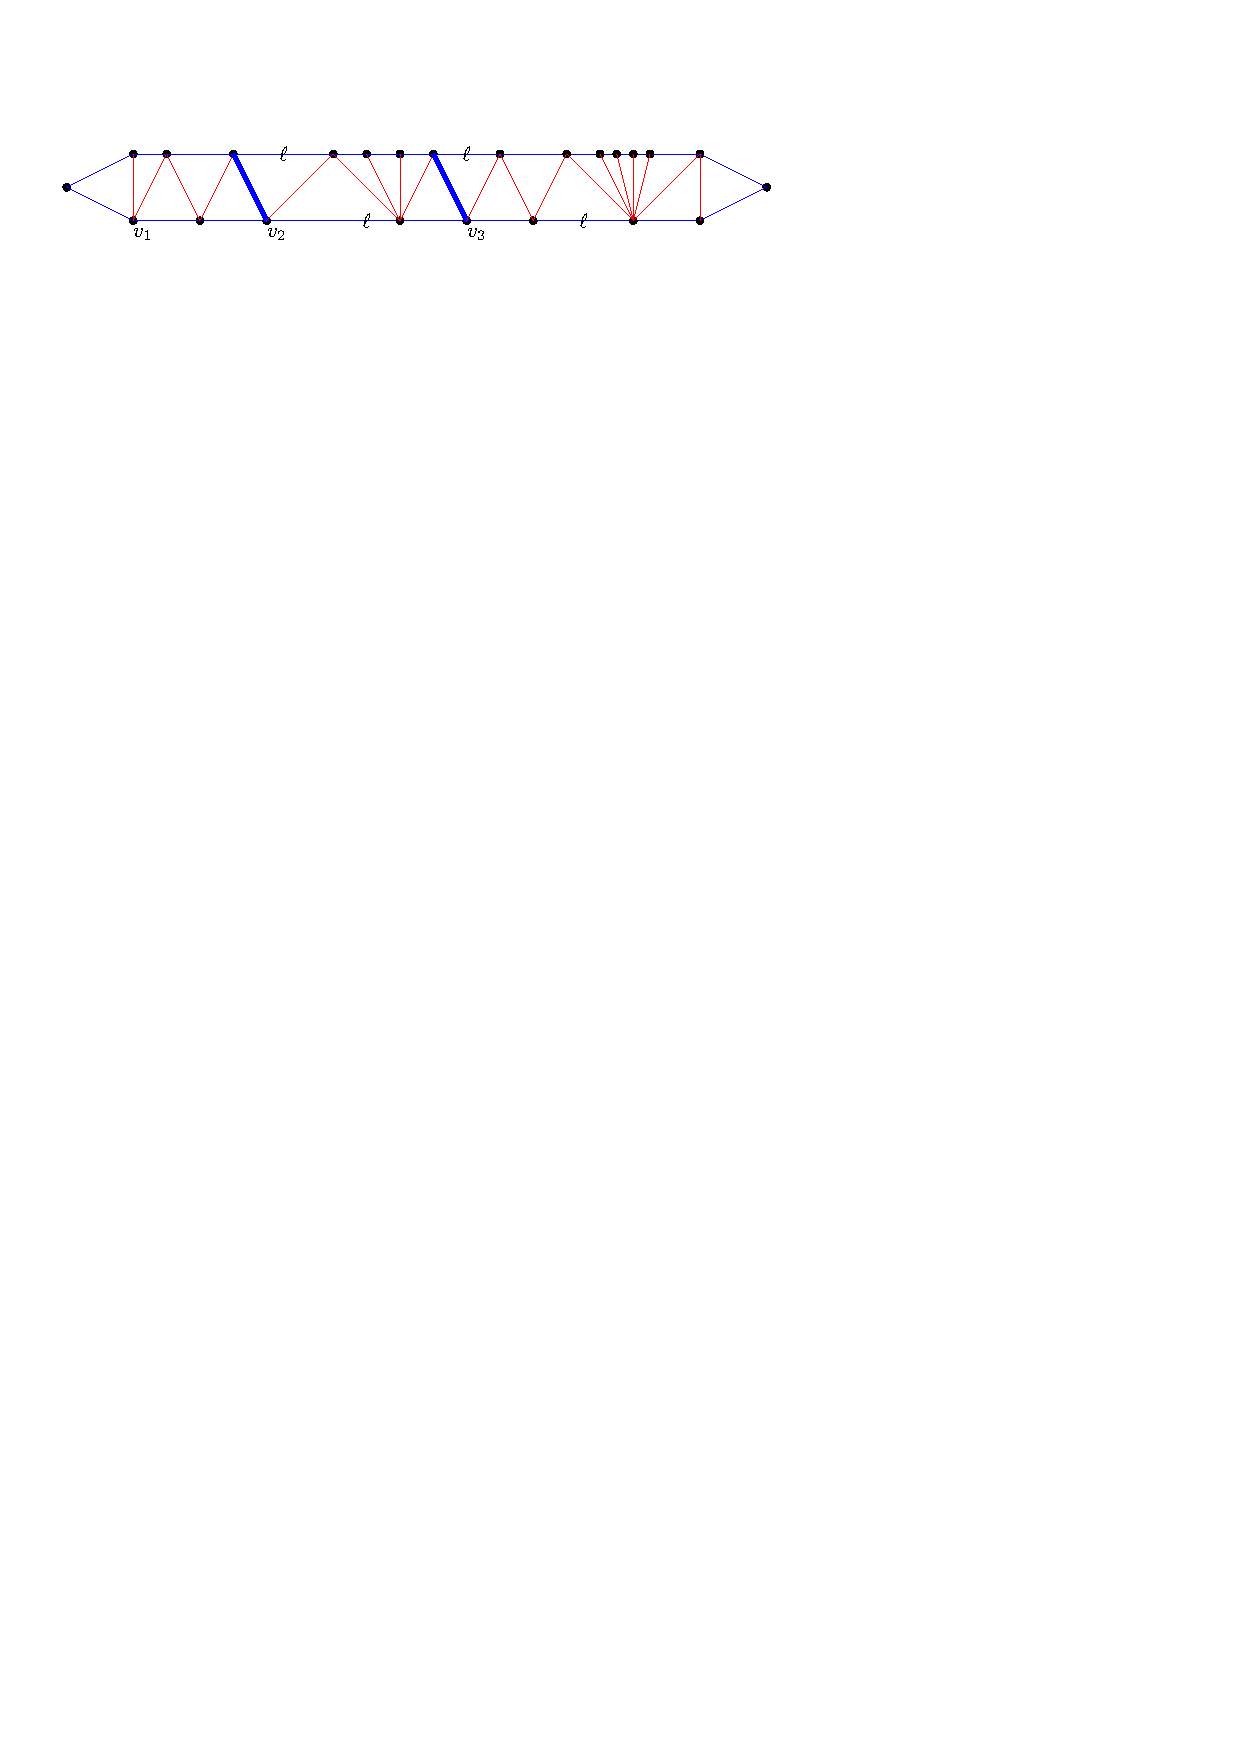
\includegraphics[scale=1]{blueFaceSubdivision/img/sampleExecution}
\clearpage% page: 46
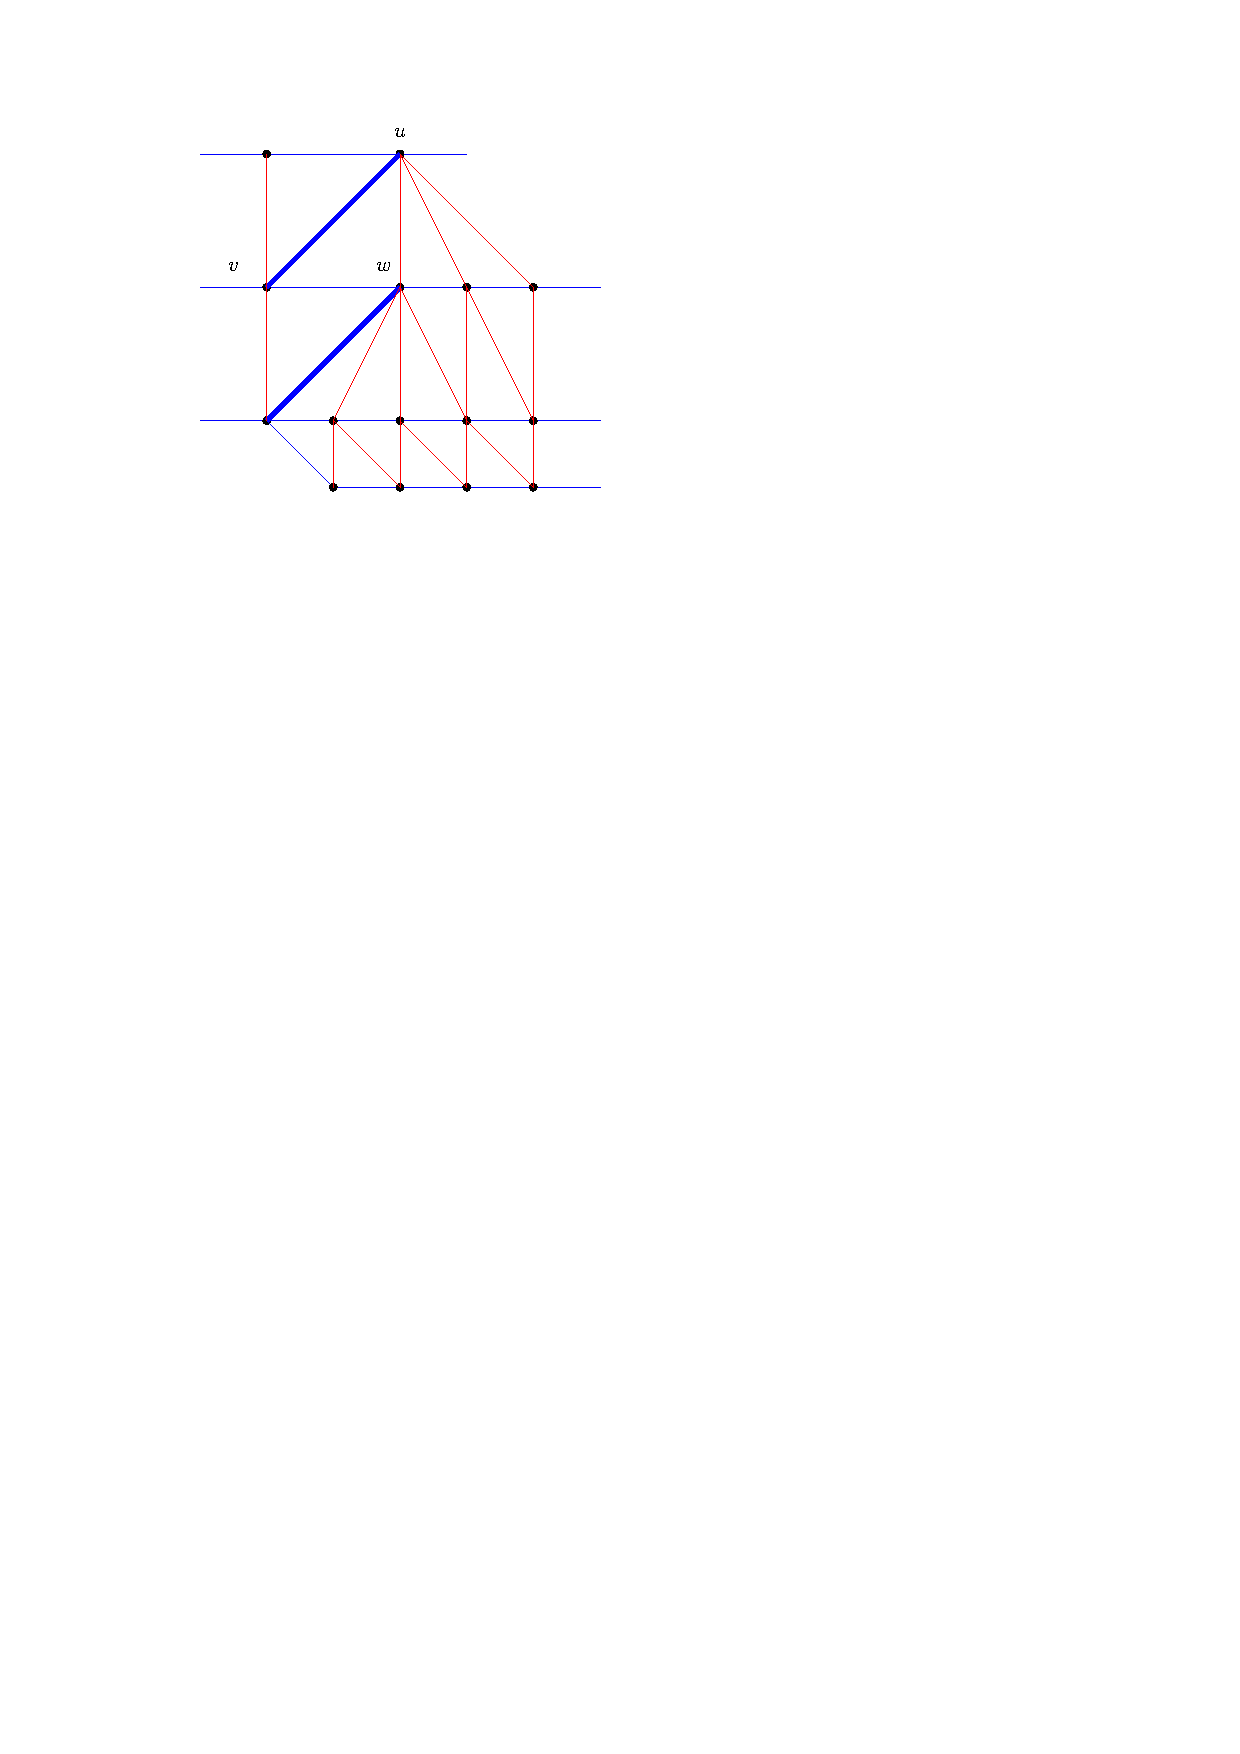
\includegraphics[scale=1]{./blueFaceSubdivision/img/forcedFlips.pdf}
\clearpage% page: 47
%Options: 
\end{document}
